\documentclass{report}

\usepackage[english]{babel}

\usepackage{graphicx}% Needed for figure files
\usepackage{hyperref}% Gives hyperlinks
\usepackage{amsmath,amsthm,amssymb}% Extra maths stuff
\usepackage{enumitem} % For a,b,c,... bullet points 
\usepackage{longtable} % Split long tables over many pages
\usepackage{lscape} % For rotating certain pages to landscape

%\usepackage{nomencl} % Needed for abbreviations
%\makenomenclature

\begin{document}
\sloppy

\title{\emph{monteswitch} user manual \\ (for version 1.0.0) }
\author{Tom L. Underwood}
\date{\today}
\maketitle

\addcontentsline{toc}{chapter}{About \emph{monteswitch}}
\chapter*{About \emph{monteswitch}}
\emph{monteswitch} is a package for performing lattice-switch Monte Carlo simulations. It was written by Tom L. Underwood, with the
exception of the random number generator, which was written by Takuji Nishimura, Makoto Matsumoto and Josi Rui Faustino de Sousa.

\emph{monteswitch} is issued under the MIT License. This is a permissive free software license which allows great flexibility
regarding use and modification of the software. A copy of the license can be found in the appendix of this document.


\addcontentsline{toc}{chapter}{Acknowledgements}
\chapter*{Acknowledgements}
The development of \emph{monteswitch} was supported by funding from the Engineering and Physical Sciences Research Council (EPSRC),
under the supervision of Graeme Ackland. Valuable discussions with Mikhail Mendelev, Nigel Wilding, Andrey Brukhno and Kevin Stratford 
are gratefully acknowledged.

\addcontentsline{toc}{chapter}{Disclaimer}
\chapter*{Disclaimer}
While we have endeavoured to ensure \emph{monteswitch} is free from error, we cannot guarantee this. Hence you use \emph{monteswitch}
at your own risk.

%\addcontentsline{toc}{chapter}{List of Abbreviations}
%\renewcommand{\nomname}{List of Abbreviations}
%\printnomenclature

\addcontentsline{toc}{chapter}{Conventions used in this manual}
\chapter*{Conventions used in this manual}
Throughout this manual we use:
\begin{itemize}
\item \texttt{typewriter font} to signify file and program names, command-line arguments to programs, and shell
commands and shell output. Shell commands are always provided on stand-alone lines starting with a `\verb|$|', e.g.,
\begin{verbatim}
$ echo "I am a shell command"
$ echo "So am I"
\end{verbatim}
Furthermore, long shell commands which do not fit on a single line are wrapped on to the following line without the presence of
a `\verb|$|', e.g.,
\begin{verbatim}
$ echo "I am a loooooooooooooooooooooooooooooooooooooooooooo
ooong shell command"
$ echo "I am not"
\end{verbatim}
Note however that `\verb|$|' is often used in the shell command itself. It should be clear from the context whether this is the
significance of any given `\verb|$|' or not.
\item \textbf{bold font} to signify the names of variables in input and output files for the \emph{monteswitch} programs.
\item \texttt{UPPER CASE TYPEWRITER FONT} to signify Fortran statements and variables. Note however that the \emph{monteswitch} 
source code is predominantly lower case (Fortran is case-insensitive). Furthermore, for clarity we sometimes use lower case, e.g.,
the type of a \texttt{REAL} array of size \textbf{M\_grid\_size} is signified as \texttt{REAL(M\_grid\_size)}.
\item the usual Unix conventions when describing usage of command-line arguments for a program, e.g., 
\texttt{program [-o] (-c|-d)} signifies that \texttt{program} has an optional command-line argument 
\texttt{-o}, and that one of the arguments \texttt{-c} or \texttt{-d} must be specified.
\end{itemize}


\addcontentsline{toc}{chapter}{Contents}
\tableofcontents


%%%%%%%%%%%%%%%%%%%%%%%%%%%%%%%%%%%%%%%%%%%%%%%%%%%%%%%%%%%%%%%%%%%%%%%%%%%%%%%%%%%%%%%%%%%%%%%%%%%%%%%%%%
\chapter{Introduction}
Calculating free energies is one of the most fundamental problems in materials science.
A plethora of different methods have been developed to this end, each designed with a particlular problem in mind (see, e.g., Ref. \cite{book:Frenkel}).
Unfortunately, in many cases commonly-used methods for calculating free energy differences between two solid phases cannot
achieve the accuracy required for many practical applications with reasonable computational effort.
One consequence of this is that the location of coexistence curves between such phases, i.e., the `lines' on a phase diagram
where the free energy difference between the two phases is zero, cannot be accurately resolved if the phases
have `very similar' free energies. This problem is by no means limited to `realistic' models of particle interactions, but
persists even when simple models are used. For instance it was only relatively recently that it was shown that the fcc crystal is
favoured over the hcp crystal in the hard-sphere solid -- an archetype of a simple system \cite{Bruce_1997,Bruce_2000,Jackson_2002}.

\emph{Lattice-switch Monte Carlo} (LSMC) \cite{Bruce_1997,Bruce_2000} 
\footnote{The reader should be aware that LSMC has also been refered to as lattice-\emph{switching} Monte Carlo.}
is a method which can be used to efficiently evaluate the free energy difference between two solid phases.
It has been applied to a wide range of systems \cite{Bruce_1997,Pronk_1999,Mau_1999,Bruce_2000,Jackson_2002,Jackson_2007,Yang_2008,
Marechal_2008,Raiteri_2010,Wilms_2012,Quigley_2014,Bridgwater_2014,Underwood_2015},
beginning with the hard-sphere solid, where it was used to resolve the aforementioned hcp--fcc problem \cite{Bruce_1997,Bruce_2000},
as well as to evaluate the free energy cost associated with stacking faults \cite{Pronk_1999,Mau_1999}. 
The method was later applied to soft interatomic potentials \cite{Jackson_2002,Wilms_2012,Underwood_2015}, 
systems containing multiple particle species \cite{Jackson_2007,Yang_2008}, and molecular systems 
\cite{Marechal_2008,Raiteri_2010,Quigley_2014,Bridgwater_2014}.
LSMC has also inspired \emph{phase switch Monte Carlo}, a method for calculating the free energy difference between a solid and a
fluid phase \cite{Wilding_2000}, which has also seen some use
\cite{Wilding_2000,Errington_2004,McNeil-Watson_2006,Wilding_2009_MP,Wilding_2009_JCP,Sollich_2010,Wilding_2010}.
%
As well as being versatile, LSMC is an accurate method: it is `exact' in the sense that it relies upon no approximations other than those present in 
the model of particle interactions it is used in conjunction with. Moreover for the purposes of evaluating the free energy difference between 
pairs of solid phases LSMC is ostensibly more efficient than all other existing methods \cite{Wilms_2012,Marechal_2008}. 
\footnote{However it should be noted that this remains somewhat of an open question \cite{Pronk_1999,Sweatman_2015}. Nevertheless one can say that LSMC is 
\emph{at least} as efficient as existing methods.}
However, despite its strengths, LSMC has unfortunately yet to have gained widespread popularity. This stems in part from the lack of 
an LSMC code which is both widely available and applicable to a wide range of systems.

With this in mind we have developed a package, \emph{monteswitch}, which implements the LSMC method. The package, written in Fortran 95, can
be used to evaluate free energy differences between pairs of solid phases in the NVT and NPT ensembles. Furthermore the
package contains a version of the main executable which is parallelised using MPI for HPC applications.
Note that the two `phases' under consideration need not be homogeneous crystals. For instance \emph{monteswitch} can be used to evaluate the
free energy cost associated with crystallographic defects. Furthermore \emph{monteswitch} can treat systems containing multiple species of particles.
However it should be noted that \emph{monteswitch} can only treat `atomic' systems (i.e., `non-molecular' systems: those in which the constituent
particles do not have rotational degrees of freedom), and pairs of phases which can be represented by orthorhombic unit cells.

While steps have been recently been taken to implement LSMC in an existing general-purpose code,
\footnote{Specifically, LSMC is earmarked for inclusion in the general-purpose Monte Carlo code \emph{DL\_MONTE} \cite{Purton_2013}.}
we believe that \emph{monteswitch} will fulfill an important `gap in the market' for the foreseeable future because it was designed from 
the outset to be highly-customisable with regards to the interatomic potential. By contrast general-purpose codes tend to have a fixed set 
of interatomic potentials to draw upon.
In \emph{monteswitch} all of the procedures pertaining to the interatomic potential are housed within a single Fortran module. 
It is intended that users write their own version of this module which implements the interatomic potential they are 
interested in.
\footnote{Of course, in doing this the user's module is free to interface with `external' modules, or even external programs.}
(A similar scheme is utilised in the molecular dynamics program MOLDY \cite{Ackland_2011}). 
Templates are provided with \emph{monteswitch} to assist with this. Furthermore modules are included
with \emph{monteswitch} which correspond to some commonly-used interatomic potentials, which can serve as examples. Of course these modules can also be
used within \emph{monteswitch} to perform LSMC calculations.

This document describes how to use \emph{monteswitch}. Note that this document does not provide details regarding the structure of the source code. 
We direct readers interested in this to the HTML source code documentation -- which can be generated from the source code (see Chapter
\ref{chapter:preliminaries}) -- or failing that the source code itself. Here we assume that the reader is already competent with the Unix shell, 
including utilities such as \texttt{grep}, \texttt{sed} and \texttt{awk}. Often we provide examples of commands which utilise the shell and the 
aforementioned utilities to perform certain tasks. However we never describe exactly how these commands work for the sake of brevity; interested users
should consult the relevant documentation online or elsewhere. In a similar vein, when we describe Fortran-related issues we assume the reader has 
an expertise in Fortran 95. We also assume that the user is familiar with the Monte Carlo method (in the sense of computational
chemistry), but not necessarily with LSMC. For further information regarding Monte Carlo simulations in condensed 
matter physics, see, e.g., Ref. \cite{book:Frenkel}. 

The layout of this document is as follows. In Chapter \ref{chapter:background} we describe the theory behind LSMC to a depth which enables the user to 
competently perform LSMC simulations using \emph{monteswitch}.
In Chapter \ref{chapter:preliminaries} we describe how to install \emph{monteswitch}, and provide
an overview of the package. In Chapter \ref{chapter:simulation_programs} we describe the main Monte Carlo programs within
\emph{monteswitch}. In Chapter \ref{chapter:interactions} we describe the various interatomic potentials included with \emph{monteswitch}, as well as
how users can implement their own potentials. In Chapter \ref{chapter:utility_programs} we describe the various utility
programs included with \emph{monteswitch} for the creation of input files and post-processing of output files. In Chapter \ref{chapter:example}
we provide a worked example which elucidates how \emph{monteswitch} can be used to solve a `real' problem. Finally in Chapter \ref{chapter:tests}
we describe the test cases included with \emph{monteswitch} which, as well as validating \emph{monteswitch}, serve as an archive of examples
for users.




%%%%%%%%%%%%%%%%%%%%%%%%%%%%%%%%%%%%%%%%%%%%%%%%%%%%%%%%%%%%%%%%%%%%%%%%%%%%%%%%%%%%%%%%%%%%%%%%%%%%%%%%%%
\chapter{Background theory}\label{chapter:background}
In this chapter we describe the LSMC methodology as relevant to \emph{monteswitch}. Further information regarding different incarnations of
LSMC can be found in the LSMC studies cited in the previous chapter.

\section{Calculating free energy differences}
Consider a system which is free to visit two phases 1 and 2 (and only phases 1 and 2).
Of phases 1 and 2, the equilibrium phase is that with the lower free energy $\mathcal{F}$, where $\mathcal{F}$ is the Helmholtz free energy $F$ in the 
NVT ensemble and the Gibbs free energy $G$ in the NPT ensemble. It is the free energy difference between the phases 
$\Delta\mathcal{F}\equiv \mathcal{F}_1-\mathcal{F}_2$ which we wish to evaluate, where $\mathcal{F}_1$ and $\mathcal{F}_2$ denote the free energies of 
phases 1 and 2.
We now derive an expression relating $\Delta \mathcal{F}$ to the probabilities $p_1$ and $p_2$ of the system being in phases 1 and 2 respectively.
It is this expression which is ultimately used in LSMC to calculate $\Delta \mathcal{F}$. Consider the free energy of phase $\alpha$:
\begin{equation}\label{Falpha_def}
\mathcal{F}_{\alpha}=-\beta^{-1}\ln Z_{\alpha},
\end{equation}
where
\begin{equation}\label{Zalpha_def}
Z_{\alpha}=\sum_{\sigma\in\alpha}\exp(-\beta \mathcal{E}_{\sigma})
\end{equation}
is the partition function for phase $\alpha$; $\beta\equiv 1/(k_BT)$; $k_B$ is Boltzmann's constant; $T$ is the temperature; 
$\sigma$ denotes a state of the system; $\mathcal{E}_{\sigma}$ denotes the energy $E_{\sigma}$ of state $\sigma$ in the NVT ensemble, and the enthalpy 
$H_{\sigma}=E_{\sigma}+PV_{\sigma}$ of state $\sigma$ in the NPT ensemble, where $V_{\sigma}$ denotes the volume of state $\sigma$; 
and the summation in the above equation is over all states which `belong' to phase $\alpha$. 
From Eqn. \eqref{Falpha_def} it follows that
\begin{equation}\label{DeltaF_Z}
\Delta \mathcal{F}=\beta^{-1}\ln\biggl(\frac{Z_2}{Z_1}\biggr).
\end{equation}
Now,
\begin{equation}\label{MC_prob}
p_{\sigma}=\frac{1}{Z}e^{-\beta \mathcal{E}_{\sigma}}, \quad Z\equiv Z_1+Z_2
\end{equation}
is the probability that the system, free to explore both phases 1 and 2, is in state $\sigma$. Hence the probability of the system being in
phase $\alpha$ is
\begin{equation}
p_{\alpha} = \sum_{\sigma\in \alpha}p_{\sigma} = Z_{\alpha}/Z,
\end{equation}
where we have used Eqn. \eqref{Zalpha_def}. Finally, substituting this into Eqn. \eqref{DeltaF_Z} gives
\begin{equation}\label{DeltaF_stat_mech}
\Delta \mathcal{F}=\beta^{-1}\ln\biggl(\frac{p_2}{p_1}\biggr).
\end{equation}

With the above equation in mind, the following method can be used to calculate $\Delta\mathcal{F}$ from a simulation which samples the ensemble under 
consideration, e.g., a molecular dynamics simulation: measure the relative time $t_1$ and $t_2$ which the system spends in each phase 1 and 2 during the
simulation, and substitute these quantities into the above equation, bearing in mind that $t_2/t_1=p_2/p_1$ for a sufficiently long simulation.
However, this method is often intractable in practice for two solid phases, 
because the time taken for the system to transition between the two phases is too long to allow a reasonable estimate of $p_2/p_1$ to be deduced 
in a reasonable simulation time; it may be the case that, regardless of the phase in which the simulation is initialised, the system \emph{never} 
transitions to the `other' phase during the course of the simulation.
The problem is that, while the regions of phase space corresponding to phase 1 and phase 2 both correspond to probable states of the system
at thermodynamic equilibrium, these regions are separated by a \emph{free energy barrier} -- a region of phase space associated
with states which are very improbable at thermodynamic equilibrium. This barrier inhibits transitions between the `islands of
stability' in phase space associated with phase 1 and phase 2.

This problem can in principle be circumvented within the Monte Carlo method.
In the original incarnation of Monte Carlo, which we refer to as \emph{canonical Monte Carlo}\cite{Metropolis_1953} (which we contrast later to 
\emph{multicanonical Monte Carlo}), the system is evolved throughout the simulation as follows. Each timestep we generate a trial state of the system 
$\sigma'$, and attempt to change the system from its current state $\sigma$, to the trial state. 
The traditional approach for NVT ensembles is to perform a `particle move' to generate a trial state. Here, one particle in $\sigma$ is moved
to yield $\sigma'$. In NPT ensembles particle moves are supplemented by `volume moves', in which the volume, and potentially shape, of the 
entire system is altered, along with a commensurate rescaling of the particle positions. We accept the change of state from $\sigma$ to $\sigma'$ with 
a probability $p_{\sigma\to\sigma'}$, which is a function of the energies of the states $\sigma$ and $\sigma'$ in the NVT ensemble, and
the enthalpies and volumes of the states $\sigma$ and $\sigma'$ in the NPT ensemble. The function also depends on the specific scheme used to generate 
state $\sigma'$ from $\sigma$. For the schemes used in \emph{monteswitch}, $p_{\sigma\to\sigma'}$ is given by
\begin{equation}\label{p_Metropolis}
p_{\sigma\to\sigma'}=\text{max}\Bigl[1,e^{\beta(E_{\sigma'}-E_{\sigma})}\Bigr]
\end{equation}
for particle moves and
\begin{equation}\label{p_Metropolis_NPT}
p_{\sigma\to\sigma'}=\text{max}\Bigl[1,e^{\beta(H_{\sigma'}-H_{\sigma})+(N+1)\ln(V_{\sigma'}/V_{\sigma})}\Bigr],
\end{equation}
for volume moves.
\footnote{See, e.g, Ref. \cite{book:Frenkel} for expressions for $p_{\sigma\to\sigma'}$ for other schemes}. 
The end result is that each state $\sigma$ is sampled with a probability which reflects the underlying ensemble, i.e., Eqn. \eqref{MC_prob}.
Hence the equilibrium value of any physical quantity $X$ can be obtained by evaluating the average of $X$ over all timesteps in a sufficiently long 
simulation. In this manner $t_1$ and $t_2$, and hence $\Delta \mathcal{F}$ (via Eqn. \eqref{DeltaF_stat_mech}) can be calculated; 
$t_{\alpha}$ is the time average of the quantity $\theta_{\alpha}$, where $\theta_{\alpha}=1$ if the system is in phase $\alpha$ and 0 otherwise.
However, in canonical Monte Carlo one has considerable freedom as to how trial states are generated; one is by no means limited to the aforementioned 
`traditional' move set. The prospect therefore exists of generating trial states in a manner which results in the system traversing a path in phase 
space which allows $\Delta \mathcal{F}$ to be calculated relatively quickly. Such a path would involve frequent transitions between both phases 1 and 
2 by `tunnelling' through the free energy barrier separating them.


\section{Lattice switch Monte Carlo moves}\label{sec:lattice_switch}
In LSMC a new type of move, a \emph{lattice switch}, is introduced to supplement the traditional move set mentioned above. A lattice switch move takes
the system \emph{directly} from one phase to the other, bypassing any free energy barriers separating the phases. Every time a lattice switch is accepted, 
the system transitions to the `other' phase. The salient feature of the move is that the underlying `lattice' which characterises the current phase is 
`switched' for a lattice which characterises the other phase. For example if the two phases in question are fcc and hcp, then a lattice switch from an
fcc state involves switching the underlying fcc lattice for an hcp lattice, while preserving the \emph{displacements} of each particle from its associated
lattice site. 
%
To elaborate, we can characterise a given state of the system as belonging to a solid phase $\alpha$ if the positions of the particles 
`approximately' form a lattice characteristic of $\alpha$. Let $\lbrace\mathbf{R}^{(\alpha)}_i\rbrace$ denote the positions of the sites on this lattice, 
and let $\lbrace\mathbf{r}_i\rbrace$ denote the positions of the particles, where $i$ ranges from 1 to the number of particles in the system. 
The position $\mathbf{r}_i$ of particle $i$ can be expressed as follows:
\begin{equation}
\mathbf{r}_i=\mathbf{R}^{(\alpha)}_i+\mathbf{u}_i,
\end{equation}
where $\mathbf{u}_i$ is the displacement of $i$ from that lattice site. Note that the displacements $\lbrace\mathbf{u}_i\rbrace$ are necessarily small 
since the particle positions form an approximate $\alpha$ lattice (and we have chosen to label particles and lattice sites in a `sensible' manner: such 
that $\mathbf{R}_i$ is the closest lattice site to $\mathbf{r}_i$). Now, in a lattice switch from phase $\alpha$ to the `other' phase $\alpha'$ we 
transform the underlying lattice $\lbrace\mathbf{R}^{(\alpha)}_i\rbrace$ to $\lbrace\mathbf{R}^{(\alpha')}_i\rbrace$, 
\emph{while keeping the particle displacements $\lbrace\mathbf{u}_i\rbrace$ unchanged}. The result is that the trial state belongs to phase 
$\alpha'$: the positions of the particles in the trial state form an approximate $\alpha'$ lattice.

\subsection{Implementation in \emph{monteswitch}}
Of course, the above description of a lattice switch is not a complete account of how lattice switches are implemented in \emph{monteswitch} -- which
supports lattice switches which change the shape and size of the supercell, as well as the species of the particles.
%
In \emph{monteswitch} two states are provided at the start of a simulation, one for each phase. There are two functions of these states. Firstly, they 
act as prospective initial states for the simulation: if the system is to be initialised in phase 1, then the phase-1 state will be used as the initial state.
Secondly, they are used to determine the nature of the lattice switch move. We refer to these states as \emph{reference states}.
Now, in \emph{monteswitch} only orthorhombic systems can be treated. Hence we only consider orthorhombic systems here. For such systems a state 
amounts to a specification of the following: the dimensions of the supercell $L_x$, $L_y$ and $L_z$ in each Cartesian direction; either the \emph{fractional} 
positions $\lbrace\tilde{\mathbf{r}}_i\rbrace$ or the \emph{absolute} positions $\lbrace\mathbf{r}_i\rbrace$ of the particles within the supercell
(we denote fractional positions by a `$\sim$'); and the species of the particles $\lbrace S_i\rbrace$. For convenience we gather these quantites into
a tuple: $(L_x,L_y,L_z,\lbrace\tilde{\mathbf{r}}_i\rbrace,\lbrace S_i\rbrace)$ or $(L_x,L_y,L_z,\lbrace\mathbf{r}_i\rbrace,\lbrace S_i\rbrace)$ amounts to
a specification of the state of the system. With this in mind, let 
$(\mathcal{L}^{(1)}_x,\mathcal{L}^{(1)}_y,\mathcal{L}^{(1)}_z,\lbrace\tilde{\mathcal{R}}^{(1)}_i\rbrace,\lbrace\mathcal{S}^{(1)}_i\rbrace)$ and
$(\mathcal{L}^{(2)}_x,\mathcal{L}^{(2)}_y,\mathcal{L}^{(2)}_z,\lbrace\tilde{\mathcal{R}}^{(2)}_i\rbrace,\lbrace\mathcal{S}^{(2)}_i\rbrace)$ describe
the reference states for phases 1 and 2 respectively.
Without loss of generality consider now a state $\sigma=(L_x,L_y,L_z,\lbrace\mathbf{r}_i\rbrace,\lbrace s_i\rbrace)$ belonging to phase 1.
We now describe how the state $\sigma'=(L_x',L_y',L_z',\lbrace\mathbf{r}'_i\rbrace,\lbrace s'_i\rbrace)$, which results from a lattice switch from
state $\sigma$, is generated from $\sigma$ in \emph{monteswitch}. We first construct the underlying phase-1 `lattice' for $\sigma$.
The positions of the lattice sites, which we denote as $\lbrace\mathbf{R}^{(1)}_i\rbrace$, are constructed from the phase-1 reference state. Specifically, 
$\lbrace\mathbf{R}^{(1)}_i\rbrace$, transformed into fractional coordinates, is identical to the fractional positions of the particles in the phase-1 
reference state:
\begin{equation}
\mathbf{R}^{(1)}_i = \text{diag}(L_x,L_y,L_z)\tilde{\mathcal{R}}^{(1)}_i
\end{equation}
for all particles $i$, where $\text{diag}(L_x,L_y,L_z)$ denotes the $3\times 3$ matrix with $L_x$, $L_y$ and $L_z$ along the leading diagonal. We now turn
to the trial state $\sigma'$. We begin by constructing the dimensions of the supercell for $\sigma'$. The reference states for both phases are 
used to determine how the supercell is transformed during the switch. Specifically, the dimensions of the supercell for $\sigma'$ are given by
\begin{equation}
L_x'=\frac{\mathcal{L}_x^{(2)}}{\mathcal{L}_x^{(1)}}L_x, \quad 
L_y'=\frac{\mathcal{L}_y^{(2)}}{\mathcal{L}_y^{(1)}}L_y, \quad 
L_z'=\frac{\mathcal{L}_z^{(2)}}{\mathcal{L}_x^{(1)}}L_z.
\end{equation}
Hence in the lattice switch the supercell is dilated/contracted in each Cartesian dimension by the same factor as would be the case in transforming the
supercell from the phase-1 reference state to the phase-2 reference state.
Thirdly, we construct the underlying lattice for phase 2. As was the case for the underlying lattice for phase 1, the underlying lattice for phase
2, transformed into fractional coordinates, is identical to the fractional positions of the particles in the phase-2 reference state:
\begin{equation}
\mathbf{R}^{(2)}_i = \text{diag}(L_x',L_y',L_z')\tilde{\mathcal{R}}^{(2)}_i
\end{equation}
for all $i$.
Fourthly we construct the particle positions in $\sigma'$ using the particle positions in $\sigma$ and the aforementioned underlying lattices for
phases 1 and 2 as follows:
\begin{equation}
\mathbf{r}_i'=\mathbf{r}_i-\mathbf{R}^{(1)}_i+\mathbf{R}^{(2)}_i
\end{equation}
for all $i$. Note that this amounts to a transformation of the particle positions in which the underlying phase-1 lattice $\lbrace\mathbf{R}^{1}_i\rbrace$ 
is substituted for a phase-2 lattice $\lbrace\mathbf{R}^{2}_i\rbrace$ while keeping the displacement of each particle from its lattice site unchanged. 
This can perhaps be seen more clearly by reexpressing the transformation as follows:
\begin{equation}
\mathbf{r}_i=\mathbf{R}^{(1)}_i+\mathbf{u}_i \to \mathbf{r}'_i=\mathbf{R}^{(2)}_i+\mathbf{u}_i
\end{equation}
for all $i$, where
\begin{equation}
\mathbf{u}_i=\mathbf{r}_i-\mathbf{R}^{(1)}_i=\mathbf{r}'_i-\mathbf{R}^{(2)}_i
\end{equation}
is the displacement of particle $i$ from its lattice site.
Finally we transform the species of $\sigma$ (which initialy corresponding to phase 1) to correspond to phase 2:
\begin{equation}
s_i= S^{(1)}_i\to s_i'= S^{(2)}_i
\end{equation}
for all $i$.

Note that the lattice switch just described is an involution: if a lattice switch from state $\sigma$ yields state $\sigma'$, then
performing a lattice switch from state $\sigma'$ yields $\sigma$.

\section{The problem with canonical sampling in LSMC}
One might expect that by regularly making lattice switches, the system will regularly transition between phases, allowing $\Delta \mathcal{F}$ to 
be efficiently evaluated as described above. Unfortunately using canonical Monte Carlo one finds that lattice switches are too rarely accepted for 
this approach to be useful. 
%
Consider the probability of a lattice switch from state $\sigma$ to $\sigma'$ being accepted. Using the lattice switch scheme implemented in
\emph{monteswitch}, and described in the previous section, this is
\begin{equation}\label{p_LSMC_NPT}
p_{\sigma\to\sigma'}=\text{max}\Bigl[1,e^{\beta(H_{\sigma'}-H_{\sigma})+\ln(V_{\sigma'}/V_{\sigma})}\Bigr],
\end{equation}
where recall that $H_{\sigma}=E_{\sigma}+PV_{\sigma}$ denotes the enthalpy of state $\sigma$, and $V_{\sigma}$ denotes its volume. Consider for now the
case where the lattice switch preserves the volume of the system. This is necessary for the NVT ensemble, but in the NPT ensemble one has freedom to
define the switch such that it changes the volume of the system. We consider the general case later.
For a \emph{volume-preserving lattice switch}, since $V_{\sigma'}=V_{\sigma}$, the above equation reduces to
\begin{equation}\label{p_LSMC_NVT}
p_{\sigma\to\sigma'}=\text{max}\Bigl[1,e^{\beta(E_{\sigma'}-E_{\sigma})}\Bigr].
\end{equation}
This equation reveals the main cause for lattice switches being unsuccessful: the energy of the trial state $\sigma'$ generated by a 
lattice switch is almost always of much higher energy than the current state $\sigma$, leading to $p_{\sigma\to\sigma'}$ being very low. 

\section{Multicanonical Monte Carlo}
The solution to this problem is to use \emph{multicanonical Monte Carlo}\cite{Berg_1991,Berg_1992,Smith_1995} instead of canonical Monte Carlo.
\footnote{Multicanonical Monte Carlo belongs to the class of extended ensemble techniques; see, e.g., Ref. \cite{Iba_2001}.}
The former is a straightforward generalisation of the latter in which, instead of sampling from the probability distribution $p_{\sigma}$ 
(Eqn. \eqref{MC_prob}), one samples from the distribution
\begin{equation}\label{MCMC_prob}
\tilde{p}_{\sigma}=\frac{1}{\tilde{Z}}e^{-\beta \mathcal{E}_{\sigma}}e^{\eta_{\sigma}}, \quad \tilde{Z}\equiv\sum_{\sigma}e^{-\beta \mathcal{E}_{\sigma}}e^{\eta_{\sigma}},
\end{equation}
where $\eta_{\sigma}$, known as the \emph{weight function}, is chosen according to the aims of the simulation. 
Using Eqn. \eqref{MC_prob}, it can be shown that
\begin{equation}\label{MCMC_prob_2}
\tilde{p}_{\sigma}=\frac{1}{\tilde{Z}'}p_{\sigma}e^{\eta_{\sigma}}, \quad \tilde{Z}'=\sum_{\sigma}p_{\sigma}e^{\eta_{\sigma}},
\end{equation}
where note that $p_{\sigma}$ is the `true' probability of the system being in state $\sigma$. From the above it can be seen that if 
$\eta_{\sigma}>0$ then state $\sigma$ is \emph{over-sampled} relative to the true distribution. On the other hand if $\eta_{\sigma}<0$ then 
$\sigma$ is \emph{under-sampled}. 
The strength of this approach is that, through judicious choice of the weight function, one can `choose' the path the system traverses 
through phase space. To elaborate, a multicanonical Monte Carlo simulation can be regarded as a canonical Monte Carlo 
simulation, but if the energy for each state $\sigma$ were 
\begin{equation}
\tilde{\mathcal{E}}_{\sigma}=\mathcal{E}_{\sigma}-\eta_{\sigma}/\beta
\end{equation}
instead of $\mathcal{E}_{\sigma}$. Hence a multicanonical Monte Carlo simulation samples states with probabilities corresponding to, say, an NVT ensemble,
but if energy were $\tilde{\mathcal{E}}_{\sigma}$ instead of $E_{\sigma}$. Noting that since the modification to the `true' energy function, 
$-\eta_{\sigma}/\beta$, is proportional to the weight function, it can be seen that the weight function defines an additional `force' on the system 
which affects its trajectory through phase space. Therefore by choosing $\eta_{\sigma}$, one can choose the system's path through phase space. 

Of course, in a multicanonical simulation the states are not longer sampled with probabilities corresponding to the true ensemble in question -- 
which \emph{is} the case for canonical Monte Carlo. Accordingly the time average of some physical quantity $X$ throughout a long multicanonical 
Monte Carlo simulation is not equivalent to the equilibrium value of $X$ for the true ensemble, as it is in a canonical Monte Carlo
simulation. Nevertheless one can obtain the equilibrium value of $X$ from a multicanonical simulation by exploiting the fact that, since the 
weight function is known, then so is the degree of over- or under-sampling of each state. To elaborate, to evaluate the equilibrium value of 
$X$ in a canonical Monte Carlo simulation, we use the following expression:
\begin{equation}
\langle X\rangle\approx\frac{1}{\tau}\sum_{t=1}^{\tau}X(t),
\end{equation}
where $X(t)$ denotes the value of the physical quantity $X$ at timestep $t$ of the simulation, and $\tau$ denotes the total number of timesteps.
For reasons which will become clear in a moment, $\langle X\rangle$ could equivalently be expressed as
\begin{equation}
\langle X\rangle\approx\frac{\displaystyle\sum_{t=1}^{\tau}w(t)X(t)}{\displaystyle\sum_{t=1}^{\tau}w(t)}
\end{equation}
with $w(t)$ taking the same constant value for all $t$, where $w(t)$ is the \emph{weight} (not to be confused with the weight function) associated 
with the state at timestep $t$.
Now, Eqn. \eqref{MCMC_prob_2} reveals that state $\sigma$ is sampled in a multicanonical Monte Carlo simulation a factor of
$e^{\eta_{\sigma}}/\tilde{Z}'$ more often than for the true ensemble. Associating a weight $(e^{\eta_{\sigma}}/\tilde{Z}')^{-1}$ to $\sigma$ corrects for
this; the effect is that states which are over-sampled are counted less, and under-sampled states are counted more, in the evaluation of $\langle X\rangle$.
Hence the expression for $\langle X\rangle$ pertaining to a multicanonical simulation is the same as above, but with $w(t)=(e^{\eta(t)}/\tilde{Z}')^{-1}$:
\begin{equation}\label{equilX_MCMC}
\langle X\rangle\approx\frac{\displaystyle\sum_{t=1}^{\tau}e^{-\eta(t)}X(t)}{\displaystyle\sum_{t=1}^{\tau}e^{-\eta(t)}},
\end{equation}
where we have canceled the factors of $\tilde{Z}'^{-1}$ from the numerator and denominator.


\section{Multicanonical Monte Carlo in LSMC}\label{sec:multicanonical_LSMC}
How does multicanonical Monte Carlo resolve the problem that lattice switch moves are too rarely accepted to be useful? Recall that lattice switches
are usually rejected because they result in a trial state with a much higher energy.
There are, however, a small number of states `close' to those realised at equilibrium for each phase from which a lattice switch yields a 
trial state $\sigma'$ which is of comparable energy to $\sigma$. From such states a lattice switch has a good chance of being accepted.
We refer to such states as \emph{gateway states}, since they provide the key to jumping between both phases. It is these states which we wish to over-sample,
and we set the weight function accordingly. The idea is that by over-sampling these states, lattice switches are accepted reasonably often, 
enabling both phases to be explored in a reasonable simulation time. This in turn allows us to determine $t_1$ and $t_2$ (which recall are the time
averages of $\theta_1$ and $\theta_2$ defined earlier, i.e., $t_1=\langle\theta_1\rangle$ and $t_2=\langle\theta_2\rangle$) via Eqn. \eqref{equilX_MCMC},
and hence ultimately $\Delta \mathcal{F}$ via Eqn. \eqref{DeltaF_stat_mech}.

How should the weight function be engineered such that gateway states are over-sampled? 
Consider a state $\sigma$, and let $\sigma'$ denote the state which results from a lattice switch performed from $\sigma$. Let us define the 
state-dependent quantity
\begin{equation}\label{M_def}
M_{\sigma}=
\begin{cases}
(E_{\sigma}-E_{\sigma'}) & \text{if $\sigma$ belongs to phase 1} \\
-(E_{\sigma}-E_{\sigma'}) & \text{if $\sigma$ belongs to phase 2}.
\end{cases}
\end{equation}
This quantity provides a practical means for resolving gateway states, states corresponding to equilibrium (for the true ensemble under consideration)
for phase 1, and states corresponding to equilibrium for phase 2. Accordingly we refer to $M$ as the \emph{order parameter}. Consider first gateway states.
Above we illustrated that gateway states correspond to the condition $E_{\sigma}\approx E_{\sigma'}$. As can be seen from the above this corresponds to
states with $M_{\sigma}\approx 0$. By contrast, if $|M_{\sigma}|\gg 0$, then the two states have significantly different values of $E$. In this case, while
switching from the state with the higher value of $E$ to that with the lower value of $E$ is guaranteed, the converse is not: the two states are not 
concordant with switching \emph{to and from} both phases. $|E_{\sigma}|$ therefore provides a measure of how `un-gateway-like' state $\sigma$ is, with 
zero corresponding to `very gateway-like'. 
Consider now phase-1-equilibrium states. From such states we generally expect a lattice switch to be unsuccessful, and hence
$E_{\sigma'}\gg E_{\sigma}$. Therefore for such states $M_{\sigma}\ll 0$. Finally consider phase-2-equilibrium states. Similarly we generally expect 
a lattice switch from such states to be unsuccessful, and hence $E_{\sigma'}\gg E_{\sigma}$. However this time $M_{\sigma}\gg 0$. 
We therefore have three regimes: $M_{\sigma}\ll 0$ corresponds to phase-1-equilibrium states; $M_{\sigma}\approx 0$ corresponds to gateway states; and 
$M_{\sigma}\gg 0$ corresponds to phase-2-equilibrium states.

With this in mind, if we choose the weight function $\eta_{\sigma}$ to take the same value $\eta_{M}$ 
for all states with the same $M$, and also choose $\eta_{M}$ to be peaked at $M=0$ and to decay monotonically with 
$|M|$, then the weight function corresponds to a `force' which drives the system towards gateway states, allowing the system to transition between
the phase-1 and phase-2 regions of phase space, corresponding to $M\ll 0$ and $M\gg 0$ respectively, in a reasonable simulation time.
This is, of course, just a \emph{qualitative} description of a form for $\eta_{M}$ which is sufficient for our purposes. As one might expect, 
the quantitative details of the weight function $\eta_{M}$ strongly affect the efficiency of the path traversed though phase space with regards 
to calculating $\Delta \mathcal{F}$; a `bad' weight function might result in the system getting stuck in one phase, or an unimportant region of phase 
space, for a long time. Furthermore, it is not obvious \emph{a priori} what a suitable weight function for a given system should be. Hence one must 
\emph{generate} a weight function which leads to an efficient sampling of phase space. After this \emph{weight function generation simulation},
the resulting weight function can be used in a \emph{production simulation} to calculate $\Delta \mathcal{F}$ as described earlier.

However in practice one cannot treat $M$ as an unbounded continuous variable as above; one cannot define an arbitrary weight function in computer
memory via this scheme. Hence in practice one considers a finite range of $M$ which is divided into $N_{\text{macro}}$ bins, each 
corresponding to a distinct range of `$M$-space'. Each bin itself corresponds to a macrostate: the macrostate is the collection of states corresponding to the 
range of $M$-space covered by the bin. We will henceforth explicitly take this discretisation of $M$ into account, and let $\mathcal{M}$ denote the 
macrostate corresponding to the $\mathcal{M}$th bin, where $\mathcal{M}=1,2,\dotsc,N_{\text{macro}}$. Accordingly let 
$\eta_{\mathcal{M}}$ denote the weight function for macrostate $\mathcal{M}$.

However this raises the question of what range of $M$ should be considered for a given problem, as well as what value $N_{\text{macro}}$ should take.
With regards to the first question, the range should be large enough to cover all states which are reasonably likely to occur at thermodynamic
equilibrium for both phases, as well as the gateway states. This is necessary because allowing the production simulation to visit the equilibrium states for 
both phases is essential in order to accurately determine the free energy difference between the two phases (as well as any thermodynamic quantities 
associated with each individual phase), while allowing the simulation to visit gateway states is essential to allow transitions between the two phases
via lattice switches. On the other hand the range should not be too large. Assuming that an ideal weight function is used, in which case the considered
range of $M$-space is sampled uniformly in the production simulation, then using too large a range lowers the efficiency of the simulation because 
it forces the system to spend less time in the regions of order-parameter space associated with equilibrium states -- which are the important states with
regards to evaluating thermodynamic quantities.
%
Regarding what value $N_{\text{macro}}$ should take, note that $N_{\text{macro}}$ determines the fineness of the grid on $M$-space upon which
the weight function is defined. Note also that the weight function is flat over the region of $M$-space corresponding to one macrostate. Furthermore, the 
higher $N_{\text{macro}}$, the finer the grid. Hence if the grid is coarse, i.e., if $N_{\text{macro}}$ is small, then there will be large regions of $M$-space
over which the weight function is flat, including near $M=0$. This is problematic because a rapidly-changing weight function is required near $M=0$ to 
`guide' the system over the free energy barrier. Thus if $N_{\text{macro}}$ is too small then the free energy barrier may prove insurmountable despite the
use of multicanonical sampling. This problem can be avoided if a sufficiently large $N_{\text{macro}}$ is used, however the larger $N_{\text{macro}}$ the
longer the simulation time required to generate the weight function. Hence a balance must be struck when choosing an appropriate value of $N_{\text{macro}}$.

\subsection{Volume-altering lattice switches}
So far we have considered volume-preserving lattice switches. However, \emph{monteswitch} supports lattice switches which alter the volume of the system.
How does the above discussion differ for \emph{volume-altering} lattice switches? The answer is `not much'. For the
case of volume-preserving lattice switches a gateway state is a state from which a lattice switch yields another state of comparable energy.
This reflects the fact that $p_{\sigma\to\sigma'}\approx 1$ if $E_{\sigma'}\approx E_{\sigma}$ in Eqn. \eqref{p_LSMC_NVT}. For the case of a
volume-altering lattice switch the analogous condition for a gateway state, as can be seen from Eqn. \eqref{p_LSMC_NPT}, is that
$J_{\sigma}\approx J_{\sigma'}$, where
\begin{equation}
J_{\sigma}\equiv H_{\sigma}+\ln(V_{\sigma})/\beta.
\end{equation}
Note that for the case of volume-preserving lattice switches the condition $J_{\sigma}\approx J_{\sigma'}$ is equivalent to $E_{\sigma}\approx E_{\sigma'}$.
Accordingly in \emph{monteswitch} the following definition of $M_{\sigma}$ is in fact used, instead of Eqn. \eqref{M_def}:
\begin{equation}
M_{\sigma}=
\begin{cases}
(J_{\sigma}-J_{\sigma'}) & \text{if $\sigma$ belongs to phase 1} \\
-(J_{\sigma}-J_{\sigma'}) & \text{if $\sigma$ belongs to phase 2}.
\end{cases}
\end{equation}


\section{Weight function generation methods}\label{sec:weight_generation}
We will now describe how weight functions can be generated for use in a production simulation.
In multicanonical Monte Carlo the `ideal' weight function, which we denote as $\eta_{\mathcal{M}}^*$, is regarded as that which leads to 
all macrostates within the considered order parameter range to be sampled with equal probability in the multicanonical Monte Carlo simulation.
Let $\tilde{p}_{\mathcal{M}}$ denote the probability that the multicanonical Monte Carlo simulation is in macrostate $\mathcal{M}$; formally,
\begin{equation}
\tilde{p}_{\mathcal{M}}=\sum_{\sigma\in\mathcal{M}}\tilde{p}_{\sigma}.
\end{equation}
Thus $\eta_{\mathcal{M}}^*$ would yield $\tilde{p}_{\mathcal{M}}=C$ for all $\mathcal{M}$ within the allowed range, where $C$ is some constant.
$\eta^*_{\mathcal{M}}$, or at least a close estimate of it, can be determined using various methods; below we 
describe the methods supported by \emph{monteswitch}. 
However we emphasise that strictly speaking it is unnecessary to use the ideal weight function, which samples all macrostates with exactly equal 
probablility, during the
production simulation. The choice of weight function affects the accuracy of physical quantities determined during the production simulation
(evaluated using Eqn. \eqref{equilX_MCMC}) only in that it determines the efficiency with which phase space is explored. For this reason though a
weight function close to the ideal is desirable because it is a convenient way of ensuring that gateway states are visited often, hence 
allowing both phases to be explored regularly: a weight function which is `far from ideal' may not result in gateway states being visited often
enough to enable useful estimates of $t_1$ and $t_2$ to be obtained. However, using the latter weight function would enable useful estimates 
for $t_1$ and $t_2$ to be obtained \emph{eventually}.

\subsection{Visited states method}\label{sec:visited_states}
The \emph{visited states method} (see Ref. \cite{Smith_1995} and references therein) is arguably the simplest method for generating the weight function. 
In this method, the simulation consists of a number of
`blocks', which themselves consist of a large number of Monte Carlo sweeps. Multicanonical sampling is used throughout, and the weight function is updated at
the end of each block. The weight function is different -- closer to the ideal -- in each subsequent block, and the number of visits to all macrostates
during each block is used to inform the weight function to be used in the next block. Eventually the weight function converges on the 
ideal: it provides a `flat' macrostate histogram; the weight function is such that all macrostates are sampled with equal probability.

Let $\mathcal{C}^{(n)}_{\mathcal{M}}$ denote the number of states belonging to macrostate $\mathcal{M}$ which were visited during block $n$.
The specific equation used to obtain the weight function for the next block $n+1$ is
\begin{equation}
\eta^{(n+1)}_{\mathcal{M}}=\eta^{(n)}_{\mathcal{M}}-\ln\Biggl\lbrace
\frac{\mathcal{C}^{(n)}_{\mathcal{M}}+1}{\sum_{\mathcal{M}'}\bigl(\mathcal{C}^{(n)}_{\mathcal{M}'}+1\bigr)}
\Biggr\rbrace
+k,
\end{equation}
where $\eta^{(n)}_{\mathcal{M}}$ denotes the weight function for block $n$; the summation over $\mathcal{M}'$ on the denominator of the fraction is
over all macrostates $1,2,\dotsc,N_{\text{macro}}$; and $k$ is an inconsequential arbitrary constant, which we choose such that the minimum value of 
$\eta^{(n+1)}_{\mathcal{M}}$ over all $\mathcal{M}$ is 0.
\footnote{Like energies, only differences in the values of the weight function between states are `physically significant'; the absolute values 
of the weight function are not. Hence performing a global shift to the weight function for our own convenience is inconsequential to the
multicanonical distribution $\tilde{p}_{\sigma}$. This can be seen by applying the transformation $\eta_{\sigma}\to\eta_{\sigma}+C$ to Eqn. \eqref{MCMC_prob},
where $C$ is an arbitrary constant}
The above equation acts to enhance the value of the weight function for macrostates which have not been visited often during the previous block, and
diminish the weight function for macrostates which have been visited. Eventually the weight function is such that all macrostates are visited equally
often. 
With regards to the choice of initial weight function for the simulation, i.e., $\eta^{(0)}_{\mathcal{M}}$, we use $\eta^{(0)}_{\mathcal{M}}=1$
for all $\mathcal{M}$. 

In practice the visited states method converges to the ideal weight function very slowly, and is not amenable to parallelisation. 
For this reason we do not recommend that it is the sole method used to 
generate weight function with \emph{monteswitch}. We recommend that the other methods for generating weight functions described 
in a moment are used instead, at least at first. These other methods are much more efficient at obtaining a weight function close to the ideal. 
However, these methods, as implemented in \emph{monteswitch}, perhaps never converge on the ideal, while the visited states method does \cite{Smith_1995}. 
This limitation of the other methods is in practice probably
unimportant. As mentioned earlier, it is unnecessary to use the `exact' ideal weight function, just a weight function `close' to the ideal, which
these methods provide. Nevertheless the visited states method is included within \emph{monteswitch} in order that the exact ideal weight function can
be calculated if required, possibly after a weight function close to the ideal has already been obtained using the aforementioned faster methods.


\subsection{Transition matrix method}\label{sec:transition_matrix}
$\eta_{\mathcal{M}}^*$ can be related to $p_{\mathcal{M}}$, the \emph{canonical} probability of the system being in macrostate $\mathcal{M}$. (Multicanonical
quantities are signified by a `$\sim$'). Firstly, note that the multicanonical probability $\tilde{p}_{\mathcal{M}}$ of the system being in macrostate 
$\mathcal{M}$ given a weight function $\eta_{\mathcal{M}}$ is
\begin{equation}
\tilde{p}_{\mathcal{M}}\propto e^{\eta_{\mathcal{M}}}p_{\mathcal{M}}.
\end{equation}
This follows from Eqn. \eqref{MCMC_prob_2}: summing over all $\sigma\in\mathcal{M}$ on the left-hand expression, and recalling that 
$\eta_{\sigma}=\eta_{\mathcal{M}}$ for such $\sigma$. Applying the condition $\tilde{p}_{\mathcal{M}}=A$ for $\eta_{\mathcal{M}}=\eta_{\mathcal{M}}^*$ yields
\begin{equation}
A\propto e^{\eta^*_{\mathcal{M}}}p_{\mathcal{M}},
\end{equation}
which can be rearranged to give
\begin{equation}\label{ideal_wf}
\eta^*_{\mathcal{M}}=A'-\ln p_{\mathcal{M}},
\end{equation}
where $A'$ is a constant. Eqn. \eqref{ideal_wf} reveals that $\eta^*_{\mathcal{M}}$ can be derived from $p_{\mathcal{M}}$. $p_{\mathcal{M}}$ 
in turn can be determined from the \emph{macrostate transition probability matrix} $\mathcal{T}_{\mathcal{MM}'}$, which describes the probability that
the system, currently in macrostate $\mathcal{M}$, transitions to macrostate $\mathcal{M}'$ \emph{in the canonical ensemble}.
In the \emph{transition matrix method} \cite{Smith_1995,Fitzgerald_1999} we determine $\mathcal{T}_{\mathcal{MM}'}$, and then use this to obtain
$p_{\mathcal{M}}$, and finally the ideal weight function $\eta_{\mathcal{M}}^*$ via Eqn. \eqref{ideal_wf}.

How do we determine $\mathcal{T}_{\mathcal{MM}'}$, and how do we obtain $p_{\mathcal{M}}$ from $\mathcal{T}_{\mathcal{MM}'}$? Let us first deal with how
$\mathcal{T}_{\mathcal{MM}'}$ is determined.
Surprisingly $\mathcal{T}_{\mathcal{MM}'}$, a canonical quantity, can be obtained from a simulation utilising canonical sampling, multicanonical sampling,
or even more exotic methods. Consider the case of canonical sampling first.
Here, $\mathcal{T}_{\mathcal{MM}'}$ can be determined in an intuitive manner as follows. During the simulation we keep track of the 
number of observed transitions between all pairs of macrostates, which we store in a matrix $\mathcal{C}_{\mathcal{M}\mathcal{M}'}$ -- where $\mathcal{C}_{\mathcal{M}\mathcal{M}'}$
denotes the number of observed transitions from macrostate $\mathcal{M}$ to macrostate $\mathcal{M}'$. We then use $\mathcal{C}_{\mathcal{M}\mathcal{M}'}$ to obtain
an estimate for $\mathcal{T}_{\mathcal{M}\mathcal{M}'}$ via the equation
\begin{equation}\label{T_estimate}
\mathcal{T}_{\mathcal{M}\mathcal{M}'}\approx \frac{\mathcal{C}_{\mathcal{M}\mathcal{M}'}+1}
{\displaystyle\sum_{\mathcal{M}^{\prime\prime}}\bigl(\mathcal{C}_{\mathcal{M}\mathcal{M}^{\prime\prime}}+1\bigr)}.
\end{equation}
However, this procedure is never used in \emph{monteswitch} because the following superior alternative exists. Consider a trial state $\sigma'$ 
generated from $\sigma$ which, if accepted, would take the system from macrostate $\mathcal{M}$ to macrostate $\mathcal{M}'$, and let the probability 
of the move being accepted be $p_{\sigma\to\sigma'}$. Instead of performing the update $\mathcal{C}_{\mathcal{M}\mathcal{M}'}\to \mathcal{C}_{\mathcal{M}\mathcal{M}'}+1$ if the move is 
accepted and $\mathcal{C}_{\mathcal{M}\mathcal{M}'}\to \mathcal{C}_{\mathcal{M}\mathcal{M}'}$ if it is not, one can perform the update 
\begin{equation}
\begin{split}
\mathcal{C}_{\mathcal{M}\mathcal{M}'}\to \mathcal{C}_{\mathcal{M}\mathcal{M}'}+p_{\sigma\to\sigma'} \\
\mathcal{C}_{\mathcal{M}\mathcal{M}}\to \mathcal{C}_{\mathcal{M}\mathcal{M}}+1-p_{\sigma\to\sigma'}
\end{split}
\end{equation} 
regardless of whether it is accepted or not. In this case $\mathcal{C}_{\mathcal{M}\mathcal{M}'}$ is no longer the number of observed transitions from macrostate 
$\mathcal{M}$ to $\mathcal{M}'$, but is instead the number of \emph{inferred} transitions. 
In fact, as alluded to above, this procedure can be used in conjunction with a multicanonical simulation, so long as one bears in mind that
$p_{\sigma\to\sigma'}$ is the \emph{canonical} probability of transitioning from state $\sigma$ to $\sigma'$ -- a quantity which is trivial to calculate
during a multicanonical simulation.
Why would one wish to use multicanonical sampling instead of canonical sampling to obtain $\mathcal{T}_{\mathcal{MM}'}$, which after all is a canonical
quantity? If multicanonical sampling is used, while the canonical transition probability $p_{\sigma\to\sigma'}$ is used to update $\mathcal{C}_{\mathcal{M}\mathcal{M}'}$
via the above equation, it is the multicanonical transition probability $\tilde{p}_{\sigma\to\sigma'}$, which depends on the weight functions of
$\sigma$ and $\sigma'$ ($\eta_{\mathcal{M}}$ and $\eta_{\mathcal{M}'}$ respectively), which is actually used to determine whether the move is accepted or not.
This is useful because canonical sampling alone may not be sufficient to explore the full range of macrostates $\mathcal{M}$, which is necessary to 
`fill up' the matrix $\mathcal{C}_{\mathcal{M}\mathcal{M}'}$ and ultimately enable $\mathcal{T}_{\mathcal{M}\mathcal{M}'}$ to be calculated (Eqn. \eqref{T_estimate}). 
For instance, typically canonical sampling will never result in the macrostates containing gateway states being visited during a reasonable simulation
time.
One can take this idea further and even go beyond multicanonical sampling to sample $M$-space. We discuss methods for exploring the $M$-space
with the aim of determining $\mathcal{T}_{\mathcal{MM}'}$, and ultimately $\eta_{\mathcal{M}}^*$, in a moment.

Having determined  $\mathcal{T}_{\mathcal{MM}'}$, our task is to now calculate $p_{\mathcal{M}}$. It can be shown that the macrostates obey the following
detailed balance condition \cite{Smith_1995}:
\begin{equation}
\mathcal{T}_{\mathcal{M}'\mathcal{M}}p_{\mathcal{M}'}=\mathcal{T}_{\mathcal{MM}'}p_{\mathcal{M}}.
\end{equation}
Setting $\mathcal{M}'=\mathcal{M}+1$ and rearranging the above gives
\begin{equation}\label{shooting}
p_{(\mathcal{M}+1)}=\frac{\mathcal{T}_{\mathcal{M}(\mathcal{M}+1)}}{\mathcal{T}_{(\mathcal{M}+1)\mathcal{M}}}p_{\mathcal{M}}.
\end{equation}
Using this equation, $p_{\mathcal{M}}$ can be obtained from the matrix $\mathcal{T}_{\mathcal{M}\mathcal{M}'}$ via the following procedure.
Firstly, one chooses some arbitrary value for $p_1$. 
\footnote{In this section $p_1$ and $p_2$ denote the probability of the system being in macrostates 1 and 2, \emph{not} the probabilities of
the system being in phases 1 and 2.}
With this $p_2$ can be obtained from the above equation ($\mathcal{M}=1$ in Eqn. \eqref{shooting}). 
This in turn can be used to obtain $p_3$ ($\mathcal{M}=2$ in Eqn. \eqref{shooting}), which in turn can be used to obtain $p_4$, etc., until
$p_{N_{\text{macro}}}$ is obtained. Finally, one normalises the resulting function $p_{\mathcal{M}}$ such that
\begin{equation}
\sum_{\mathcal{M}=1}^{N_{\text{macro}}}p_{\mathcal{M}}=1,
\end{equation}
as is required. The final step is to use $p_{\mathcal{M}}$ to obtain an estimate for the ideal weight function. This is done simply by substituting 
$p_{\mathcal{M}}$ into Eqn. \eqref{ideal_wf}. We refer to this method for obtaining the weight function as the \emph{shooting method}.
The accuracy of the resulting ideal weight function depends on how good our statistics are with regards to
the matrix $\mathcal{C}_{\mathcal{M}\mathcal{M}'}$ (specifically the elements in the diagonals immediately above and below the main diagonal), which is used to
estimate $\mathcal{T}_{\mathcal{M}\mathcal{M}'}$ via Eqn. \eqref{T_estimate}, and ultimately $\eta^*_{\mathcal{M}}$. 


\subsubsection{Methods for exploring $M$-space}
As alluded to above, since the updates to $\mathcal{C}_{\mathcal{M}\mathcal{M}'}$ always use the canonical probabilities of transitioning between states, 
with the transition matrix method one can \emph{choose} how $M$-space is explored. Effectively the only constraint is that there is fast local 
equilibration within each macrostate. We will now describe the various methods which can be implemented in \emph{monteswitch}.

The first method is to use multicanonical sampling to explore $M$-space with a continuously evolving weight function, where the weight function
at a given time is the current estimate for the ideal weight function derived from the current $\mathcal{C}_{\mathcal{M}\mathcal{M}'}$ as described above.
This is the `natural' way of applying the transition state method.

The second method is to use what we refer to as \emph{artificial dynamics} to force the system to explore all macrostates in a reasonable amount of time. 
In this method, the system is first locked into a macrostate for a certain period of time. After that period of time has elapsed, the `barriers' preventing
the system from moving into an adjacent macrostate is moved such that the system is free to transition into an adjacent macrostate. Once this occurs,
the system is locked into this new macrostate, and the procedure starts again. There is of course the question of which adjacent macrostate to `open'
to the system. Assuming we are not in macrostate $\mathcal{M}=1$ or $N_{\text{macro}}$, then there are two options: $(\mathcal{M}+1)$ and $(\mathcal{M}-1)$.
In \emph{monteswitch} one can specify whether to select the new macrostate at random \cite{thesis:Jackson}, 
or whether to sweep through the macrostates systematically, e.g., to explore macrostates 
$3,4,5,\dotsc,(N_{\text{macro}}-1),N_{\text{macro}},(N_{\text{macro}}-1),\dotsc,3,2,1,2,3,\dotsc$. This method is faster than the `natural'
method just described because one does not have to wait for the weight function to evolve such that it pushes the system to explore macrostates which
are unlikely to be visited in the canonical ensemble.




%%%%%%%%%%%%%%%%%%%%%%%%%%%%%%%%%%%%%%%%%%%%%%%%%%%%%%%%%%%%%%%%%%%%%%%%%%%%%%%%%%%%%%%%%%%%%%%%%%%%%%%%%%
\chapter{Preliminaries}\label{chapter:preliminaries}

\section{Obtaining \emph{monteswitch}}
\emph{monteswitch} is hosted on GitHub at \url{https://github.com/tomlunderwood/monteswitch}, where the package can be downloaded.


\section{Compiling \emph{monteswitch}}
\emph{monteswitch} is provided as an archive. This should be extracted to create a directory which consitutes the \emph{monteswitch} package. The 
package should then be compiled using the Make utility: see the `README' section in the file \texttt{Makefile}, which contains details regarding how to
specify the Fortran and MPI compiler and any flags used during compilation, as well as how to compile only the serial (i.e., non-MPI) programs
if the user's platform does not contain MPI.
The default paths to the Fortran and MPI compilers in \texttt{Makefile} are \texttt{gfortran} and \texttt{mpif90} respectively. For platforms in which
these paths apply \emph{monteswitch} can be compiled `out of the box' by invoking the command 
\begin{verbatim}
$ make serial
\end{verbatim} 
to compile only serial executables, or 
\begin{verbatim}
$ make mpi
\end{verbatim}
to compile \emph{all} executables.


\section{Transferability between platforms and compilers}
\emph{monteswitch} has not yet been tested on many platforms, and hence there may be unforeseen problems when implementing \emph{monteswitch} on
the user's platform. We have overwhelmingly used GFortran and Open MPI compilers with \emph{monteswitch}; hence these compilers can be considered 
to be the most `safe'.

One issue we have found with regards to using \emph{monteswitch} on different platforms stems from the fact that \emph{monteswitch} uses Fortran's 
list-directed input and output. This means the nature of the output from \emph{monteswitch} programs is noticeably compiler-dependent. This in itself
is not a problem, though the post-processing commands given in forthcoming chapters may need to be subtly modified to work with programs compiled using 
something other than GFortran.

Another issue we have found is that the usage of the utility \texttt{sed} is platform-dependent. In particular we have found that appropriate command-line
argument to \texttt{sed} to invoke in-place editing of a file, without saving a backup, is `\texttt{-i ''}' on OS X (note the `\texttt{''}'), 
while it is simply `\texttt{-i}' on other Unix platforms (where adding `\texttt{''}' results in an error being returned by \texttt{sed} on these
platforms). This has a bearing on the transferability of some of the \texttt{run.sh} shell scripts in the directory \texttt{Tests} -- which correspond to the
OS X version of \texttt{sed} -- to the user's platform. Hence the user should ensure that these scripts are appropriate for their platform, and modify
them accordingly if not.


\section{Package overview}
After compilation, the \emph{monteswitch} directory will contain the following programs:
\begin{itemize}
\item\texttt{monteswitch}
\item\texttt{monteswitch\_mpi}
\item\texttt{monteswitch\_post}
\item\texttt{lattices\_in\_hcp\_fcc}
\item\texttt{lattices\_in\_bcc\_fcc}
\item\texttt{lattices\_in\_bcc\_hcp}
\end{itemize}
\texttt{monteswitch} and \texttt{monteswitch\_mpi} are the key programs of the package: they perform Monte Carlo simulations. 
By contrast \texttt{monteswitch\_post}, \texttt{lattices\_in\_hcp\_fcc}, \texttt{lattices\_in\_bcc\_fcc} and 
\texttt{lattices\_in\_bcc\_hcp} are utility programs: \texttt{monteswitch\_post} is for post-processing one of the output files created 
by the main programs; and \texttt{lattices\_in\_hcp\_fcc}, \texttt{lattices\_in\_bcc\_fcc} and \texttt{lattices\_in\_bcc\_hcp} are for generating 
one of the input files for the main programs. We will elaborate upon the function of each of these programs later.

\subsection{Test cases and examples}
There are a number of subdirectories within the package. The directory \texttt{Tests} contains a suite of test cases for the main programs. 
Chapter \ref{chapter:tests} contains descriptions of the tests, including how to run each test and what results 
to expect. We recommend that the tests be performed by the user to ensure that the Monte Carlo programs, as compiled by their system, work
correctly. Furthermore, these tests are also instructive, providing examples of how to perform various tasks which the typical user would be 
interested in performing. Finally, the tests serve to validate the Monte Carlo programs by illustrating that they reproduce known results.

While the test cases serve as examples, more pedagogical examples can be found in the directory \texttt{Examples}, including the worked example
of Chapter \ref{chapter:example}.

\subsection{Specifying the interatomic potential}\label{sec:plugins}
The file \texttt{interactions.f95} in the main directory of the package contains the Fortran module, named \texttt{interactions\_mod}, which
determines the interatomic potential to be utilised by the \emph{monteswitch} programs \texttt{monteswitch}, \texttt{monteswitch\_mpi} and
\texttt{monteswitch\_post} after the package is compiled. 
%
By default \texttt{interactions.f95} corresponds to the EAM model; however the directory  \texttt{Interactions} contains versions of 
\texttt{interactions.f95} which implement various interatomic potentials, as well as templates which assist the user in creating their own
versions of \texttt{interactions.f95}. 
%
To implement a specific interatomic potential one must copy the corresponding \texttt{interactions.f95} file to \texttt{interactions.f95} 
in the main directory of the package, and then compile the package. Further information regarding this is provided in Chapter \ref{chapter:interactions}.


\section{Source code documentation}
HTML documentation for the source code can be generated from `marked-up' comments in the source code files. Invoking the command 
\begin{verbatim}
$ make srcdocs
\end{verbatim}
generates this documentation: each HTML file corresponds to a particular source code file.


%%%%%%%%%%%%%%%%%%%%%%%%%%%%%%%%%%%%%%%%%%%%%%%%%%%%%%%%%%%%%%%%%%%%%%%%%%%%%%%%%%%%%%%%%%%%%%%%%%%%%%%%%%
\chapter{Monte Carlo simulation programs}\label{chapter:simulation_programs}
The key programs in the package are \texttt{monteswitch} and \texttt{monteswitch\_mpi}.
The main purpose of these programs is to perform LSMC simulations, though they can also
be used to perform `conventional' Monte Carlo simulations. \texttt{monteswitch\_mpi} is the MPI-parallelised analogue of \texttt{monteswitch}. 
While in \texttt{monteswitch} one simulation is performed, in \texttt{monteswitch\_mpi} multiple simulations are 
performed in parallel. These simulations are identical except for the seed used for the random number generator. Hence \texttt{monteswitch\_mpi}
is simply a convenient means to exploit parallelisation in order to obtain results quickly. Further details regarding the parallelisation
are provided later in Section \ref{sec:monteswitch_mpi}.
%
In terms of usage and simulation methodology \texttt{monteswitch} and \texttt{monteswitch\_mpi} are almost identical. For this reason we 
focus on \texttt{monteswitch} below, where it should be assumed that what is said for \texttt{monteswitch\_mpi} also applies for
\texttt{monteswitch\_mpi} unless otherwise stated.

\section{Overview of functionality}
\texttt{monteswitch} can treat phases which can be represented by orthorhombic supercells in the NVT and NPT ensembles, where in the
NPT ensemble both isotropic volume moves and volume moves which allow the shape of the system to alter are supported. Multicomponent
systems are allowed, however \texttt{monteswitch} cannot treat `molecular' systems in which the particles have orientational degrees of
freedom: rotational Monte Carlo moves are not implemented in \texttt{monteswitch}.

\texttt{monteswitch} supports both canonical and multicanonical sampling, where the multicanonical
sampling is performed over the LSMC order parameter described in Section \ref{sec:multicanonical_LSMC}.
Regarding weight function generation, \texttt{monteswitch} supports all of the methods described in Section \ref{sec:weight_generation}. 
Note that the option to perform canonical sampling enables conventional Monte Carlo simulations to be performed. 
Note also that, like all other LSMC implementations the authors are aware of, \texttt{monteswitch} explicitly keeps track of two states of 
the system during a simulation, one corresponding to phase 1 and one corresponding to phase 2. At any point during the simulation only one 
of these is the `actual' state of the system $\sigma$, while the other is the state $\sigma'$ which would result if a lattice switch were
performed from $\sigma$. For instance if the system were in phase 1, then $\sigma$ would belong to phase 1 and $\sigma'$ would belong to 
phase 2. During a simulation the actual state $\sigma$ is evolved via particle moves, and additionally volume moves for the case of the NPT ensemble, 
in the conventional manner. However the `other' state $\sigma'$ is evolved contemporaneously with $\sigma$ so that $\sigma'$ is always what 
would result if a lattice switch were performed from $\sigma$. It is necessary to continuously track $\sigma'$ in this manner because the LSMC order 
parameter for $\sigma$ depends on the energy, and possibly also the volume, of $\sigma'$ (see Section \ref{sec:multicanonical_LSMC} for details). 
Regarding lattice switch moves, if such a move is accepted, then the actual state is simply relabelled from $\sigma$ to $\sigma'$, while $\sigma$ is 
relabelled as the `other' state. Always keeping track of two states as just described has a downside: while optimal for LSMC simulations, 
it is not optimal for conventional Monte Carlo simulations -- where keeping track of another state is unnecessary. Thus \texttt{monteswitch} will 
typically be twice as slow for conventional Monte Carlo simulations relative to an analogous program which would only keep track of one state during 
a conventional Monte Carlo simulation.

\texttt{monteswitch} also supports on-the-fly evaluation of physical quantities and their uncertainties during the simulation via block 
averaging (see, e.g., Ref. \cite{book:Frenkel}, and Section \ref{sec:block_averaging} later). It also supports the ability to check whether or not 
the system has `melted', i.e., whether or not one or more of the particles have strayed `too far' from their lattice sites. In a similar vein, 
it is possible in \texttt{monteswitch} to perform simulations in the centre-of-mass reference frame, which provides a means of suppressing spurious
melting due to `drift' in the centre-of-mass of the system during the simulation.

The random number generator utilised by \texttt{monteswitch} is the Mersenne Twister (MT19937) \cite{Matsumoto_1998}.


\section{Command-line arguments}
The command-line arguments passed to \texttt{monteswitch} determine the nature of the invoked simulation. Usage of \texttt{monteswitch} is as follows: 
\begin{verbatim}
monteswitch [-seed <seed>] -new [-wf]
monteswitch [-seed <seed>] (-resume|-reset)
\end{verbatim}
Note that one, and only one, of the arguments \texttt{-new}, \texttt{-resume} and \texttt{-reset} must be specified,
while the arguments \texttt{-seed} and \texttt{-wf} are optional (where moreover \texttt{-wf} can only be used in conjunction with \texttt{-new}) . 
Note also that the order of the arguments is important: if \texttt{-seed} is specified then it must be the first argument; if
\texttt{-wf} is specified it must be the last argument. Below we describe the function of each of these arguments.


\section{Seeding the random number generator: the argument \texttt{-seed}}
The command-line argument \texttt{-seed} allows the user to explicitly specify the seed for the random number generator for the forthcoming simulation. 
If \texttt{-seed} is present, then the following argument \texttt{<seed>}
is taken to be the seed. For example, to set the seed to 12345 for a simulation using the \texttt{-new}
argument (whose function will be explained in a moment) the appropriate command is \texttt{monteswitch -seed 12345 -new}.
If the argument \texttt{-seed} is absent then a seed is generated using the system clock.


\section{Starting a new simulation: the argument \texttt{-new}}
The command-line argument \texttt{-new} invokes a new simulation `from scratch'. In this case
the simulation is initialised using information contained in input files located in the current directory. The input files required
by \texttt{monteswitch} will depend on the specific version of \texttt{interactions.f95} utilised when compiling \emph{monteswitch} 
(see Section \ref{sec:plugins}). 
However it is only the input files which contain information pertaining to the interatomic potential which are version-dependent;
the remaining information used to initialise a simulation are read from input files which are universal to all versions of 
\texttt{monteswitch}, namely \texttt{lattices\_in}, \texttt{params\_in} and \texttt{wf\_in}. We defer discussion of the
input files for the interatomic potential to Chapter \ref{chapter:interactions}, focusing here on \texttt{lattices\_in}, 
\texttt{params\_in} and \texttt{wf\_in}. The first two of these are compulsory: they are read by all new simulations. 
By contrast \texttt{wf\_in} is optional, only being read if the command-line argument \texttt{-wf} is present (see above for usage). 
We now describe the format and purpose of these files.


\subsection{Input file: \texttt{lattices\_in}}\label{sec:lattices_in}
The input file \texttt{lattices\_in} contains specifications for two states (i.e., supercell dimensions and particle positions), one for
each phase. These two states are the reference states described in Section \ref{sec:lattice_switch}. Recall that they serve two purposes. Firstly,
they act as prospective initial state for the simulation: if the system is to be initialised in phase 1, then the phase-1 state will be used as 
the initial state, and similarly if the system is to be initialised in phase 2. Secondly they determine the nature of the lattice switch; see
Section \ref{sec:lattice_switch} for details.
The format of \texttt{lattices\_in} is as follows. The 1st line is a comment line, and is ignored by the main programs. The 2nd line contains
the number of particles $N$ in both phases (and must be the same for both phases). The 3rd, 4th and 5th lines contain the dimensions of the
supercell for phase 1 in the x-, y- and z-directions respectively. The next $N$ lines contain the species and positions of the particles within 
the supercell for phase 1 \emph{in fractional coordinates}: each line contains the fractional x-, y- and z-coordinates for the particle, followed 
by an integer which signifies its species. (A particle's species potentially determines how it interacts with other particles; \emph{monteswitch} 
allows different interatomic potentials between sets of particles belonging to different species. The specifics of this are determined by the file 
\texttt{interactions.f95} -- see Chapter \ref{chapter:interactions}). The remaining lines in \texttt{lattices\_in} similarly specify the state 
for phase 2: the next 3 lines contains the dimensions of the supercell for phase 2 in the x-, y- and z-directions respectively; and the next $N$ 
lines contain the fractional positions and species of the particles for phase 2.

Below is an example of a \texttt{lattices\_in} file corresponding to phase 1 being an 8-particle bcc supercell and phase 2 being an 8-particle hcp 
supercell, where the phase-1 state consists entirely of particles belonging to species `1'and the phase-2 state consists of a mixture of species `1'
and `2'. Further examples of \texttt{lattices\_in} files can be found in the \texttt{Tests} and \texttt{Examples} directories.
\begin{verbatim}
 bcc-hcp, rho = 0.5, nx,ny,nz = 1, 1, 2
   8
 2.2449241     
 1.5874012     
 4.4898482
   0.0000000   0.0000000   0.0000000   1
   0.5000000   0.5000000   0.0000000   1
   0.5000000   0.0000000   0.2500000   1
   0.0000000   0.5000000   0.2500000   1
   0.0000000   0.0000000   0.5000000   1
   0.5000000   0.5000000   0.5000000   1
   0.5000000   0.0000000   0.7500000   1
   0.0000000   0.5000000   0.7500000   1
 2.4494897     
 1.4142136     
 4.6188021     
   0.0000000   0.0000000   0.0000000   1
   0.5000000   0.5000000   0.0000000   2
   0.3333333   0.0000000   0.2500000   1
   0.8333333   0.5000000   0.2500000   2
   0.0000000   0.0000000   0.5000000   1
   0.5000000   0.5000000   0.5000000   2
   0.3333333   0.0000000   0.7500000   1
   0.8333333   0.5000000   0.7500000   2
\end{verbatim}
Bearing in mind our description of the lattice switch utilised in \emph{monteswitch} given in Section \ref{sec:lattice_switch}, it can be seen that
the above file results in the following lattice switch from phase 1 to 2:
\begin{itemize}
\item A scaling of the x-dimension of the supercell by a factor of $\mathcal{L}_x^{(2)}/\mathcal{L}_x^{(1)}=2.2449/2.2449=1$, i.e., not at all.
\item A scaling of the y-dimension of the supercell by a factor of $\mathcal{L}_y^{(2)}/\mathcal{L}_y^{(1)}=1.414/1.587=0.891$.
\item A scaling of the z-dimension of the supercell by a factor of $\mathcal{L}_z^{(2)}/\mathcal{L}_z^{(1)}=4.619/4.490=1.029$.
\item A transformation of the fractional position of the underlying lattice site for particle $i$ from the $i$th fractional position specified in the file
for phase 1 to the $i$th fractional position specified for phase 2. E.g. the underlying lattice site for particle 3 has its fractional position
$(0.5000000,0.0000000,0.2500000)$ transformed to $(0.3333333,0.0000000,0.2500000)$.
\item A transformation of the species of particles 2, 4, 6 and 8 from `1' to `2'.
\end{itemize}
The lattice switch from phase 2 to 1 is the inverse of the above transformation.


\subsection{Input file: \texttt{params\_in}}\label{section:params_in}
The input file \texttt{params\_in} contains the variables which determine the nature of the simulation. Each variable corresponds to a
specific single line in the file, and each line must consist of an arbitrary string (we recommend the name of the variable followed immediately
by an `=' character with no spaces), followed by whitespace, followed by the value of the variable. To illustrate this, below is an excerpt from a 
\texttt{params\_in} file:
\begin{verbatim}
init_lattice=                            1
M_grid_size=                             100
M_grid_min=                              -82.0
M_grid_max=                              48.0
enable_multicanonical=                   T
beta=                                    9.403
P=                                       0.0
enable_lattice_moves=                    T
enable_part_moves=                       T
enable_vol_moves=                        T
part_select=                             "rand"
part_step=                               0.3
enable_COM_frame=                        T
vol_dynamics=                            "UVM"
vol_freq=                                1
vol_step=                                0.03
stop_sweeps=                             160000
equil_sweeps=                            0
enable_melt_checks=                      T
melt_sweeps=                             100
melt_threshold=                          3.0
melt_option=                             "zero_current"
\end{verbatim}
The variables which must appear in a \texttt{params\_in}, as well as a description of their function, are given in Table \ref{table:params_in_variables}. 
\emph{Note that the variables must appear in params\_in in the order that they appear in the table}. E.g., the first 
variable must be \textbf{init\_lattice}, the second must be \textbf{M\_grid\_size}, etc. Examples of \texttt{params\_in} files can
be found in the \texttt{Tests} and \texttt{Examples} directories, which can serve as templates for the user.
%
Note that by `move' we mean one of either a: particle move, in which one particle is moved to generate a trial microsate; a lattice move, in 
which the lattice is switched; and a volume move, in which the unit cell itself is altered. Furthermore if the move is rejected then it is 
still deemed to have taken place. For an NVT ensemble with lattice moves enabled the following move `cycle' is performed: particle move, 
lattice move. For an NPT ensemble with lattice moves enabled the move cycle is: particle move, lattice move, (volume move, lattice move), 
where the set of moves in the brackets occur on average \textbf{vol\_freq} times per sweep, where a `sweep' consists of $N$ move cycles,
where $N$ is the number of particles in the system.

\begin{landscape}
\begin{center}\label{table:params_in_variables}
\begin{longtable}{l l l p{8cm}}
\caption{Control variables for \texttt{monteswitch}, and descriptions of their functions. These variables must be specified in the \texttt{params\_in} file, 
one per line, in the order specified in the table. `Line' refers to the line number in \texttt{params\_in} on which the corresponding variable must appear.}
\\

Line & Variable & Type & Description \\
\hline
1 & \textbf{init\_lattice}  &  \texttt{INTEGER}  & Starting phase for the simulation (1 or 2). \\
2 & \textbf{M\_grid\_size}  &  \texttt{INTEGER}  & Number of macrostates to divide the considered order parameter range (\textbf{M\_grid\_min} to 
\textbf{M\_grid\_max}) into. \emph{This must be greater than 1}. \\
3 & \textbf{M\_grid\_min}  &  \texttt{REAL}  & Minimum of considered order parameter range. Note that moves which take the system outwith the considered 
range are automatically rejected. In other words, the system is constrained to have an order parameter between \textbf{M\_grid\_min} and 
\textbf{M\_grid\_max}. Hence
if one wants to perform a simulation in which the order parameter is unconstrained, one should set \textbf{M\_grid\_min} and \textbf{M\_grid\_max} to
values which would never be realised by the system, e.g., $-1\times 10^{100}$ and $1\times 10^{100}$ respectively. This would be the case if one wishes
to use \texttt{monteswitch} to perform a conventional Monte Carlo simulation. \\
4 & \textbf{M\_grid\_max}  &  \texttt{REAL}  & Maximum of considered order parameter range. (See also comments for \textbf{M\_grid\_min}).  \\
5 & \textbf{enable\_multicanonical}  &  \texttt{LOGICAL}  & \texttt{T} enables multicanonical sampling using the current weight function; \texttt{F} 
enables canonical sampling. \\
6 & \textbf{beta}  &  \texttt{REAL}  & Inverse temperature: $\beta=1/(k_BT)$, where $k_B$ is the Boltzmann constant.  \\
7 & \textbf{P}  &  \texttt{REAL}  & Pressure (only relevant in NPT ensemble simulations).  \\
8 & \textbf{enable\_lattice\_moves}  &  \texttt{LOGICAL}  & \texttt{T} enables lattice switch moves (performed after evey particle and volume move). \\
9 & \textbf{enable\_part\_moves}  &  \texttt{LOGICAL}  & \texttt{T} enables particle moves. This should probably be set to \texttt{T}; however disabling 
particle moves and enabling volume moves may be useful for `relaxing' the volume of the system before simulations with particle moves are performed. \\
10 & \textbf{enable\_vol\_moves}  &  \texttt{LOGICAL}  & \texttt{T} enables volume moves and selects the NPT ensemble; \texttt{F} selects the NVT ensemble. 
A volume move will be attempted on average \textbf{vol\_freq} times per sweep. \\
11 & \textbf{part\_select}  &  \texttt{CHARACTER(30)}  & Flag determining how the next particle to move is selected: \texttt{"cycle"} selects particles 
sequentially, \texttt{"rand"} selects particles at random.  \\
12 & \textbf{part\_step}  &  \texttt{REAL}  & Particle move maximum size; particles are moved according to a random walk, with a maximum move size of 
\textbf{part\_step} in any Cartesian direction.  \\
13 & \textbf{enable\_COM\_frame}  &  \texttt{LOGICAL}  & \texttt{T} performs the simulation in the centre-of-mass reference frame; \texttt{F} uses 
the lab frame. Using the centre-of-mass frame prevents `drift' in the centre-of-mass, which is convenient because it keeps particles close to
their lattice sites. However there is a computational overhead associated with using the centre-of-mass frame. \\
14 & \textbf{vol\_dynamics}  &  \texttt{CHARACTER(30)}  & Flag determining which type of volume moves are performed: \texttt{"FVM"} (fixed volume move) 
keeps the supercell shape unchanged during a volume move; \texttt{"UVM"} (unconstrained volume move) allows the x-, y- and z-dimensions to move 
independently. \\
15 & \textbf{vol\_freq}  &  \texttt{INTEGER}  & Number of volume moves performed per sweep on average if volume moves are enabled.
We recommend that this be set to 1.\\
16 & \textbf{vol\_step}  &  \texttt{REAL}  & Volume move maximum step size; the volume is moved according to a random walk in `$\ln(V)$-space', with a 
maximum move size of \textbf{vol\_step}.  \\
17 & \textbf{stop\_sweeps}  &  \texttt{INTEGER}  & Total number of sweeps to perform in the simulation. If this is set to 0 then no Monte Carlo moves 
are performed, but tasks performed periodically during the Monte Carlo loop (i.e, updating the weight function, checking whether or not the system has 
melted, checking for `divergences' in the energy, calculating equilibrium quantities and their uncertainties) are performed. \\
18 & \textbf{equil\_sweeps}  &  \texttt{INTEGER}  & Number of sweeps to disregard before the system is considered to be equilibrated; statistics are not 
gathered during these sweeps for block averaging (see below). \\
19 & \textbf{enable\_melt\_checks}  &  \texttt{LOGICAL}  & \texttt{T} enables periodic checks of whether the system has `melted', i.e., if one or 
more of the particles has moved more than a distance of \textbf{melt\_threshold} from its lattice site in any Cartesian direction then the system is 
considered to have `melted'. We recommend that this feature is used, since the LSMC method relies upon the fact that the two phases under
consideration are metastable, and that particles will not move too far from their lattice sites on the timescale of the simulation. \\
20 & \textbf{melt\_sweeps}  &  \texttt{INTEGER}  & Period (sweeps) to check for melting.  \\
21 & \textbf{melt\_threshold}  &  \texttt{REAL}  & See \textbf{enable\_melt\_checks}.  \\
22 & \textbf{melt\_option}  &  \texttt{CHARACTER(30)}  & Flag determining what the simulation does if the system has `melted': \texttt{"zero\_1"} and 
\texttt{"zero\_2"} move the system to the zero-displacement states in phases 1 and 2, respectively; \texttt{"zero\_current"} does the same but for 
the current phase; \texttt{"stop"} stops the simulation with an exit status of 2. For \texttt{"zero\_1"}, \texttt{"zero\_2"}, \texttt{"zero\_current"} the 
system is allowed to re-equilibrate before statistics are gathered for bock averaging. Also, the current block is disregarded for the purposes of 
block averaging. \\
23 & \textbf{enable\_divergence\_checks}  &  \texttt{LOGICAL}  & \texttt{T} enables periodic checks of whether the energy of the system is correct. 
To elaborate, for particle 
moves, the energy of the trial state is not calculated exactly because it is very computationally expensive and unnecessary. Instead the energy 
\emph{change} with respect to the current state is calculated. This is far less demanding to calculate. If the move is accepted this change is 
\emph{amended} to the total energy. However, over time it is possible that this `running total' approach will yield incorrect energies due to the finite 
precision of the computer. Hence one should periodically recalculate the energy exactly. This is done during volume moves. If 
\textbf{enable\_divergence\_checks} is set to \texttt{T}, then this is also done every \textbf{divergence\_sweeps} sweeps, after which the 
recalculated energy 
is compared to the 'current' energy, and the simulation is stopped with an exit status of 3 if they are different -- outwith a tolerence of 
\textbf{divergence\_tol}. Note that the order parameter is also ammended after the energy (for phases 1 and 2) is recalculated. We recommend that this 
feature is used in NVT simulations, since it forces the energy of the system to be recalculated from scratch every so often. For NPT simulations this 
should not be an issue since the energy is calculated from scratch every accepted volume move. \\
24 & \textbf{divergence\_sweeps}  &  \texttt{INTEGER}  & Period (sweeps) to check for `energy divergences' as just mentioned. 
Note that checking entails recalculating the energy from scratch.  \\
25 & \textbf{divergence\_tol}  &  \texttt{REAL}  & See \textbf{enable\_divergence\_checks}.  \\
26 & \textbf{output\_file\_period}  &  \texttt{INTEGER}  & Period (sweeps) at which information is output to the file \texttt{data}. See 
Section \ref{sec:output}. \\
27 & \textbf{output\_file\_Lx}  &  \texttt{LOGICAL}  & See Section \ref{sec:output}. \\
28 & \textbf{output\_file\_Ly}  &  \texttt{LOGICAL}  & See Section \ref{sec:output}. \\
29 & \textbf{output\_file\_Lz}  &  \texttt{LOGICAL}  & See Section \ref{sec:output}. \\
30 & \textbf{output\_file\_V}  &  \texttt{LOGICAL}  & See Section \ref{sec:output}. \\
31 & \textbf{output\_file\_R\_1}  &  \texttt{LOGICAL}  & See Section \ref{sec:output}. \\
32 & \textbf{output\_file\_R\_2}  &  \texttt{LOGICAL}  & See Section \ref{sec:output}. \\
33 & \textbf{output\_file\_u}  &  \texttt{LOGICAL}  & See Section \ref{sec:output}. \\
34 & \textbf{output\_file\_lattice}  &  \texttt{LOGICAL}  & See Section \ref{sec:output}. \\
35 & \textbf{output\_file\_E}  &  \texttt{LOGICAL}  & See Section \ref{sec:output}. \\
36 & \textbf{output\_file\_M}  &  \texttt{LOGICAL}  & See Section \ref{sec:output}. \\
37 & \textbf{output\_file\_macro}  &  \texttt{LOGICAL}  & See Section \ref{sec:output}. \\
38 & \textbf{output\_file\_eta}  &  \texttt{LOGICAL}  & See Section \ref{sec:output}. \\
39 & \textbf{output\_file\_moves\_lattice}  &  \texttt{LOGICAL}  & See Section \ref{sec:output}. \\
40 & \textbf{output\_file\_accepted\_moves\_lattice}  &  \texttt{LOGICAL}  & See Section \ref{sec:output}. \\
41 & \textbf{output\_file\_moves\_part}  &  \texttt{LOGICAL}  & See Section \ref{sec:output}. \\
42 & \textbf{output\_file\_accepted\_moves\_part}  &  \texttt{LOGICAL}  & See Section \ref{sec:output}. \\
43 & \textbf{output\_file\_moves\_vol}  &  \texttt{LOGICAL}  & See Section \ref{sec:output}. \\
44 & \textbf{output\_file\_accepted\_moves\_vol}  &  \texttt{LOGICAL}  & See Section \ref{sec:output}. \\
45 & \textbf{output\_file\_rejected\_moves\_M\_OOB}  &  \texttt{LOGICAL}  & See Section \ref{sec:output}. \\
46 & \textbf{output\_file\_M\_OOB\_high}  &  \texttt{LOGICAL}  & See Section \ref{sec:output}. \\
47 & \textbf{output\_file\_M\_OOB\_low}  &  \texttt{LOGICAL}  & See Section \ref{sec:output}. \\
48 & \textbf{output\_file\_barrier\_macro\_low}  &  \texttt{LOGICAL}  & See Section \ref{sec:output}. \\
49 & \textbf{output\_file\_barrier\_macro\_high}  &  \texttt{LOGICAL}  & See Section \ref{sec:output}. \\
50 & \textbf{output\_file\_rejected\_moves\_M\_barrier}  &  \texttt{LOGICAL}  & See Section \ref{sec:output}. \\
51 & \textbf{output\_file\_moves\_since\_lock}  &  \texttt{LOGICAL}  & See Section \ref{sec:output}. \\
52 & \textbf{output\_file\_melts}  &  \texttt{LOGICAL}  & See Section \ref{sec:output}. \\
53 & \textbf{output\_file\_equil\_DeltaF}  &  \texttt{LOGICAL}  & See Section \ref{sec:output}. \\
54 & \textbf{output\_file\_sigma\_equil\_DeltaF}  &  \texttt{LOGICAL}  & See Section \ref{sec:output}. \\
55 & \textbf{output\_file\_equil\_H\_1}  &  \texttt{LOGICAL}  & See Section \ref{sec:output}. \\
56 & \textbf{output\_file\_sigma\_equil\_H\_1}  &  \texttt{LOGICAL}  & See Section \ref{sec:output}. \\
57 & \textbf{output\_file\_equil\_H\_2}  &  \texttt{LOGICAL}  & See Section \ref{sec:output}. \\
58 & \textbf{output\_file\_sigma\_equil\_H\_2}  &  \texttt{LOGICAL}  & See Section \ref{sec:output}. \\
59 & \textbf{output\_file\_equil\_V\_1}  &  \texttt{LOGICAL}  & See Section \ref{sec:output}. \\
60 & \textbf{output\_file\_sigma\_equil\_V\_1}  &  \texttt{LOGICAL}  & See Section \ref{sec:output}. \\
61 & \textbf{output\_file\_equil\_V\_2}  &  \texttt{LOGICAL}  & See Section \ref{sec:output}. \\
62 & \textbf{output\_file\_sigma\_equil\_V\_2}  &  \texttt{LOGICAL}  & See Section \ref{sec:output}. \\
63 & \textbf{output\_file\_equil\_umsd\_1}  &  \texttt{LOGICAL}  & See Section \ref{sec:output}. \\
64 & \textbf{output\_file\_sigma\_equil\_umsd\_1}  &  \texttt{LOGICAL}  & See Section \ref{sec:output}. \\
65 & \textbf{output\_file\_equil\_umsd\_2}  &  \texttt{LOGICAL}  & See Section \ref{sec:output}. \\
66 & \textbf{output\_file\_sigma\_equil\_umsd\_2}  &  \texttt{LOGICAL}  & See Section \ref{sec:output}. \\
67 & \textbf{output\_file\_equil\_L\_1} &  \texttt{LOGICAL}  & See Section \ref{sec:output}. \\
68 & \textbf{output\_file\_sigma\_equil\_L\_1} &  \texttt{LOGICAL}  & See Section \ref{sec:output}. \\
69 & \textbf{output\_file\_equil\_L\_2} &  \texttt{LOGICAL}  & See Section \ref{sec:output}. \\
70 & \textbf{output\_file\_sigma\_equil\_L\_2} &  \texttt{LOGICAL}  & See Section \ref{sec:output}. \\
71 & \textbf{output\_stdout\_period}  &  \texttt{INTEGER}  & Period (sweeps) at which information is output to stdout. See Section \ref{sec:output}. \\
72 & \textbf{output\_stdout\_Lx}  &  \texttt{LOGICAL}  & See Section \ref{sec:output}. \\
73 & \textbf{output\_stdout\_Ly}  &  \texttt{LOGICAL}  & See Section \ref{sec:output}. \\
74 & \textbf{output\_stdout\_Lz}  &  \texttt{LOGICAL}  & See Section \ref{sec:output}. \\
75 & \textbf{output\_stdout\_V}  &  \texttt{LOGICAL}  & See Section \ref{sec:output}. \\
76 & \textbf{output\_stdout\_R\_1}  &  \texttt{LOGICAL}  & See Section \ref{sec:output}. \\
77 & \textbf{output\_stdout\_R\_2}  &  \texttt{LOGICAL}  & See Section \ref{sec:output}. \\
78 & \textbf{output\_stdout\_u}  &  \texttt{LOGICAL}  & See Section \ref{sec:output}. \\
79 & \textbf{output\_stdout\_lattice}  &  \texttt{LOGICAL}  & See Section \ref{sec:output}. \\
80 & \textbf{output\_stdout\_E}  &  \texttt{LOGICAL}  & See Section \ref{sec:output}. \\
81 & \textbf{output\_stdout\_M}  &  \texttt{LOGICAL}  & See Section \ref{sec:output}. \\
82 & \textbf{output\_stdout\_macro}  &  \texttt{LOGICAL}  & See Section \ref{sec:output}. \\
83 & \textbf{output\_stdout\_eta}  &  \texttt{LOGICAL}  & See Section \ref{sec:output}. \\
84 & \textbf{output\_stdout\_moves\_lattice}  &  \texttt{LOGICAL}  & See Section \ref{sec:output}. \\
85 & \textbf{output\_stdout\_accepted\_moves\_lattice}  &  \texttt{LOGICAL}  & See Section \ref{sec:output}. \\
86 & \textbf{output\_stdout\_moves\_part}  &  \texttt{LOGICAL}  & See Section \ref{sec:output}. \\
87 & \textbf{output\_stdout\_accepted\_moves\_part}  &  \texttt{LOGICAL}  & See Section \ref{sec:output}. \\
88 & \textbf{output\_stdout\_moves\_vol}  &  \texttt{LOGICAL}  & See Section \ref{sec:output}. \\
89 & \textbf{output\_stdout\_accepted\_moves\_vol}  &  \texttt{LOGICAL}  & See Section \ref{sec:output}. \\
90 & \textbf{output\_stdout\_rejected\_moves\_M\_OOB}  &  \texttt{LOGICAL}  & See Section \ref{sec:output}. \\
91 & \textbf{output\_stdout\_M\_OOB\_high}  &  \texttt{LOGICAL}  & See Section \ref{sec:output}. \\
92 & \textbf{output\_stdout\_M\_OOB\_low}  &  \texttt{LOGICAL}  & See Section \ref{sec:output}. \\
93 & \textbf{output\_stdout\_barrier\_macro\_low}  &  \texttt{LOGICAL}  & See Section \ref{sec:output}. \\
94 & \textbf{output\_stdout\_barrier\_macro\_high}  &  \texttt{LOGICAL}  & See Section \ref{sec:output}. \\
95 & \textbf{output\_stdout\_rejected\_moves\_M\_barrier}  &  \texttt{LOGICAL}  & See Section \ref{sec:output}. \\
96 & \textbf{output\_stdout\_moves\_since\_lock}  &  \texttt{LOGICAL}  & See Section \ref{sec:output}. \\
97 & \textbf{output\_stdout\_melts}  &  \texttt{LOGICAL}  & See Section \ref{sec:output}. \\
98 & \textbf{output\_stdout\_equil\_DeltaF}  &  \texttt{LOGICAL}  & See Section \ref{sec:output}. \\
99 & \textbf{output\_stdout\_sigma\_equil\_DeltaF}  &  \texttt{LOGICAL}  & See Section \ref{sec:output}. \\
100 & \textbf{output\_stdout\_equil\_H\_1}  &  \texttt{LOGICAL}  & See Section \ref{sec:output}. \\
101 & \textbf{output\_stdout\_sigma\_equil\_H\_1}  &  \texttt{LOGICAL}  & See Section \ref{sec:output}. \\
102 & \textbf{output\_stdout\_equil\_H\_2}  &  \texttt{LOGICAL}  & See Section \ref{sec:output}. \\
103 & \textbf{output\_stdout\_sigma\_equil\_H\_2}  &  \texttt{LOGICAL}  & See Section \ref{sec:output}. \\
104 & \textbf{output\_stdout\_equil\_V\_1}  &  \texttt{LOGICAL}  & See Section \ref{sec:output}. \\
105 & \textbf{output\_stdout\_sigma\_equil\_V\_1}  &  \texttt{LOGICAL}  & See Section \ref{sec:output}. \\
106 & \textbf{output\_stdout\_equil\_V\_2}  &  \texttt{LOGICAL}  & See Section \ref{sec:output}. \\
107 & \textbf{output\_stdout\_sigma\_equil\_V\_2}  &  \texttt{LOGICAL}  & See Section \ref{sec:output}. \\
108 & \textbf{output\_stdout\_equil\_umsd\_1}  &  \texttt{LOGICAL}  & See Section \ref{sec:output}. \\
109 & \textbf{output\_stdout\_sigma\_equil\_umsd\_1}  &  \texttt{LOGICAL}  & See Section \ref{sec:output}. \\
110 & \textbf{output\_stdout\_equil\_umsd\_2}  &  \texttt{LOGICAL}  & See Section \ref{sec:output}. \\
111 & \textbf{output\_stdout\_sigma\_equil\_umsd\_2}  &  \texttt{LOGICAL}  & See Section \ref{sec:output}. \\
112 & \textbf{output\_stdout\_equil\_L\_1} &  \texttt{LOGICAL}  & See Section \ref{sec:output}. \\
113 & \textbf{output\_stdout\_sigma\_equil\_L\_1} &  \texttt{LOGICAL}  & See Section \ref{sec:output}. \\
114 & \textbf{output\_stdout\_equil\_L\_2} &  \texttt{LOGICAL}  & See Section \ref{sec:output}. \\
115 & \textbf{output\_stdout\_sigma\_equil\_L\_2} &  \texttt{LOGICAL}  & See Section \ref{sec:output}. \\
116 & \textbf{checkpoint\_period}  &  \texttt{INTEGER}  & Period (sweeps) at which the simulation is checkpointed, i.e., how often all 
simulation variables are 
output to the file \texttt{state}. If \textbf{checkpoint\_period} is $\leq 0$ then \texttt{state} will be an empty file. See Section \ref{sec:output}. \\
117 & \textbf{update\_eta}  &  \texttt{LOGICAL}  & \texttt{T} results in the weight function being periodically updated every 
\textbf{update\_eta\_sweeps} sweeps, according
to the method specified in \textbf{update\_eta\_method}; 
\texttt{F} results in the weight function not being updated -- it remains frozen at its current state.  \\
118 & \textbf{update\_eta\_sweeps}  &  \texttt{INTEGER}  & Period (sweeps) at which the weight function is updated. \\
119 & \textbf{update\_trans}  &  \texttt{LOGICAL}  & \texttt{T} results in the transition matrix being updated; 
\texttt{F} results in it not being updated.  \\
120 & \textbf{update\_eta\_method}  &  \texttt{CHARACTER(30)}  & Method used to update the weight function: \texttt{"VS"} uses the visited 
states method; \texttt{"shooting"} uses the shooting method (using the current transition matrix). (See Section \ref{sec:weight_generation}).  \\
121 & \textbf{enable\_barriers}  &  \texttt{LOGICAL}  & \texttt{T} enables artificial dynamics; for \texttt{F} the system is free to explore 
any macrostate, but is constrained to reside within the considered order parameter range (\textbf{M\_grid\_min} to \textbf{M\_grid\_max}). 
(See Section \ref{sec:weight_generation}). \\
122 & \textbf{barrier\_dynamics}  &  \texttt{CHARACTER(30)}  & Flag determining how the macrostate barriers will evolve during artificial dynamics. 
All methods lock the system into a single
macrostate for \textbf{lock\_moves} moves, before unlocking an adjacent macrostate. Once the system has moved into the adjacent macrostate, the system
is then locked into that macrostate, and the procedure starts again. \texttt{"random"} evolves the macrostate the system is locked into via a 
random walk: the
next macrostate is decided with equal probability to be that above or that below the current macrostate. \texttt{"pong\_up"} moves to increasingly higher 
macrostates until the upper limit of the supported order parameter range is encountered, at which point it reverses direction and proceeds to 
increasingly lower macrostates until it reaches the lower limit of the order parameter range, at which point it reverses direction, etc. 
\texttt{"pong\_down"}
instead moves initially to increasingly lower macrostates.  \\
123 & \textbf{lock\_moves}  &  \texttt{INTEGER}  & The number of moves to lock the system into one macrostate for if artificial dynamics is used. 
This should be greater than 0. \\
124 & \textbf{calc\_equil\_properties}  &  \texttt{LOGICAL}  & \texttt{T} enables internal calculation of various physical quantities, and associated
uncertainties, via block averaging. (See Section \ref{sec:output}). \\
125 & \textbf{block\_sweeps}  &  \texttt{INTEGER}  & The number of sweeps which comprise a `block' which will be used to evaluate physical quantities and
their associated uncertainties via block averaging (see Section \ref{sec:output}). This should be greater than 0. \\
\end{longtable}
\end{center}
\end{landscape}


\subsection{Input file: \texttt{wf\_in}}
The command-line argument \texttt{-wf} allows one to specify the initial weight function to be used in the simulation: if \texttt{-wf} is present, then
the initial weight function is read from the file \texttt{wf\_in}. If \texttt{-wf} is absent then \texttt{wf\_in} is not read, and the weight function 
is initialised to 0 for all macrostates. \texttt{wf\_in} must contain \textbf{M\_grid\_size} lines
(where \textbf{M\_grid\_size} is specified in \texttt{params\_in}), each containing two tokens (extra lines and tokens are ignored),
which both should be of type \texttt{REAL}. The first token on each line is ignored, while the second tokens are treated as the
weight function: the value of the weight function for macrostate $i$ is initialised to the value of the second token on line $i$ in
\texttt{wf\_in}. Note that the format of \texttt{wf\_in} is analogous to that output by the program \texttt{monteswitch\_post} in conjunction with the
\texttt{-extract\_wf} argument -- see Section \ref{sec:monteswitch_post}.


\section{Output: stdout, \texttt{state} and \texttt{data}}\label{sec:output}
During a simulation information is periodically output to stdout and the file \texttt{data}. The variables with names beginning with 
\textbf{output\_file\_} and \textbf{output\_stdout\_} determine which variables are output to \texttt{data} and stdout respectively.
The variable \textbf{output\_file\_X}, where \textbf{X} is the name of a simulation variable (a list is given below), when set to \texttt{T}, 
will result in a line consisting of \texttt{X: } followed by the number of completed sweeps, followed by the current value of \textbf{X} 
being printed to \texttt{data} every \textbf{output\_file\_period} sweeps. To illustrate this, below is an excerpt of a data file corresponding
to \textbf{output\_file\_period} being set to 250:
\begin{verbatim}
 Lx:          250   20.506880155055160        22.375541637220159     
 Ly:          250   21.983483940969180        19.585057663268277     
 Lz:          250   20.142474063147095        20.720990682970093     
 V:          250   9080.4825242547813     
 lattice:          250           2
 E:          250  -2420.3817246101821     
 M:          250   12.808541584236991     
 eta:          250   9.9865126253137664     
 barrier_macro_low:          250          84
 Lx:          500   20.470022712854778        22.335325610873863     
 Ly:          500   21.965084799027686        19.568665891297709     
 Lz:          500   20.294516764376276        20.877400237511747     
 V:          500   9124.9380258152232     
 lattice:          500           2
 E:          500  -2409.3469532112986     
 M:          500   1.1974997526594968     
 eta:          500   54.025947498280964     
 barrier_macro_low:          500          84
 Lx:          750   20.472567199702674        22.338101960615028     
 Ly:          750   21.653559219100391        19.291128151472556     
 Lz:          750   20.503721368631055        21.092613455213190     
 V:          750   9089.3805950278784     
 lattice:          750           1
\end{verbatim}
The exceptions are if \textbf{output\_file\_period} is set to 0, then instead the output is after every move, and if \textbf{output\_file\_period} is a 
negative integer, in which case there is no output to the file, i.e., the output is suppressed. All of the above also applies to 
\textbf{output\_stdout\_X}, but for the output to stdout.

The file \texttt{data} can be used to deduce how the system evolves with time during the simulation. For instance, one can use the information contained 
within \texttt{data} to check whether or not the system has equilibrated within a certain number of Monte Carlo sweeps. In a production simulation it
can also be used to store the `observations' performed on the system, which could be used in subsequent analysis.

In addition to \texttt{data}, a file \texttt{state} is also created by the program periodically throughout a simulation. This file contains a
snapshot of all the 
simulation variables, and can be used to `resume' the simulation by running \texttt{monteswitch} with the \texttt{-resume} or \texttt{-reset} argument
(see Sections \ref{sec:resume} and \ref{sec:reset}), or to extract the `results' of the simulation, e.g., equilibrium quantities, the current weight 
function, the number of accepted vs. rejected Monte Carlo moves of a certain type -- perhaps using the \texttt{monteswitch\_post} program 
(see Section \ref{sec:monteswitch_post}).
The variable \textbf{checkpoint\_period} determines how often the simulation is checkpointed: a file \texttt{state} is created every 
\textbf{checkpoint\_period} sweeps. It is also \emph{always} created at the completion of the program. Note that if \textbf{checkpoint\_period} is $\leq 0$, 
then there is no output to \texttt{state}, i.e., the file will be empty.
In the \texttt{state} file, similarly to \texttt{params\_in}, each line corresponds to a particular variable: for variable $X$ the corresponding line contains
\texttt{X=} followed by the value of that variable. To illustrate this, below is an except of a \texttt{state} file:
\begin{verbatim}
 output_stdout_sigma_equil_L_2=  T
 checkpoint_period=         2000
 M_grid_size=          100
 n_part=          384
 Lx=    20.828469299691541        22.726435154004815     
 Ly=    21.821584954680326        19.440822063915213     
 Lz=    20.313660823118358        20.897094137158106     
 V=    9232.7662932888543     
 lattice=            2
 E_1=   -2398.4613158910693     
 E_2=   -2417.6552334642806     
 E=   -2417.6552334642820     
 M=    19.193917573211365     
 macro=           87
 eta=    0.0000000000000000     
 switchscalex=    1.0911236359717214     
 switchscaley=   0.89089871814033939     
 switchscalez=    1.0287212294780348     
 sweeps=          200
 moves=       154044
 moves_lattice=        77022
 accepted_moves_lattice=            1
 moves_part=        76800
\end{verbatim}
A desired line can be extracted from \texttt{state} using the utility \texttt{grep}. E.g. the command
\begin{verbatim}
$ grep "E=" state
\end{verbatim}
can be used to extract the current energy of the system from \texttt{state}.
Note that \texttt{state} contains \emph{all} the simulation variables, including those
pertaining to the interatomic potential. Hence the format of \texttt{state} depends on the details of the \texttt{interactions.f95} file. However,
all variables pertaining to the interatomic potential are stored at the end of \texttt{state}. Hence the format of \texttt{state} files down to the
point where the variables pertaining to the interatomic potential are stored is universal.

Table \ref{table:state_variables} contains a list of \texttt{monteswitch} internal variables, not already covered by Table \ref{table:params_in_variables},
which have corresponding \textbf{output\_file\_} or \textbf{output\_stdout\_} flags, or can be found in \texttt{state} and could be of interest
to the user. Note that there are other variables in \texttt{state} which are not mentioned in Tables \ref{table:params_in_variables} or 
\ref{table:state_variables} -- aside from those stemming from \texttt{interactions.f95}. We do not mention them because these are not likely to be of
interest to the user; for more information see the HTML documentation for \texttt{monteswitch\_mod.f95}.
Note that the internal variable names output in \texttt{state} are case-sensitive, and exactly reflect the names given in Tables 
\ref{table:params_in_variables} and \ref{table:state_variables}.

\subsection{Block averaging}\label{sec:block_averaging}
\texttt{monteswitch} has the ability to use block averaging to provide estimates of various physical quantities on-the-fly during a simulation. 
This feature is activated by setting the variable \textbf{calc\_equil\_properties} to \texttt{T}.
In block averaging one calculates an estimate for some arbitrary physical quantity $X$, which we denote as $\bar{X}$, as well as an associated
uncertainty in $\bar{X}$, which we denote as $\sigma_X$. $\bar{X}$ and $\sigma_X$ are calculated as follows.
After the equilibration period, the simulation time is partitioned into $N_{\text{blocks}}$ `blocks' each consisting of an equal number of 
moves.
For each block $b$ we obtain an estimate for $X$ by averaging over the values of $X$ corresponding to all states visited during that block. 
Let $X_b$ denote the estimate for $X$ for block $b$ obtained in this manner. Now, by taking the average of the values of $X_b$ over all blocks, one can 
obtain an even more accurate estimate for $X$. This is $\bar{X}$: 
\begin{equation}
\bar{X}=\frac{1}{N_{\text{blocks}}}\sum_{b=1}^{N_{\text{blocks}}}X_b.
\end{equation}
The uncertainty $\sigma_X$ is simply the standard error in $\bar{X}$:
\begin{equation}
\sigma_X=\frac{1}{\sqrt{N_{\text{blocks}}}}\sqrt{\frac{1}{(N_{\text{blocks}}-1)}\sum_{b=1}^{N_{\text{blocks}}}(X_b-\bar{X})^2}.
\end{equation}

In \texttt{monteswitch} the internal variable \textbf{block\_sweeps} determines the size of a block in sweeps. Internal variables with names 
beginning with `\textbf{equil\_}' or `\textbf{sigma\_equil\_}' contain the results of block averaging.
To elaborate, \textbf{equil\_X} corresponds to $\bar{X}$ and \textbf{sigma\_equil\_X} corresponds to $\sigma_X$ calculated by \texttt{monteswitch}
for physical quantity $X$. The variables with this format can be found in Table \ref{table:state_variables}. 
These variables are updated every time a block is `completed' by the simulation after the equilibration time. Note that
the variable \textbf{block\_counts\_X} contains the number of blocks which have been used so far in evaluating \textbf{equil\_X} and 
\textbf{sigma\_equil\_X}. Hence \textbf{equil\_X} will be meaningless (i.e., uninitialised) if \textbf{block\_counts\_X} takes the value 0, and 
\textbf{sigma\_equil\_X} will be meaningless if  \textbf{block\_counts\_X} is less than 2 (in which case there have not yet been enough blocks to 
evaluate $\sigma_X$). Blocks may be `disregarded' by \texttt{monteswitch}, i.e., not used in the evaluation of \textbf{equil\_X} and 
\textbf{sigma\_equil\_X} for a number of reasons. Firstly, a block is disregarded if the system was deemed to have `melted' during the block
(see \textbf{enable\_melt\_checks} in Table \ref{table:params_in_variables}). Secondly, a block is disregarded if during the block the system
never visits the phase or phases necessary to calculate $X$. For instance if $X$ is the volume of phase 1, then $X$ can only be evaluated if
phase 1 is actually visited during the block. Accordingly in this case a block in which phase 1 is never visited is disregarded for the 
purposes of calculating $X$. Another important example is if $X$ is the free energy difference between the two phases. In this case $X$
can only be evaluated if both phases are visited during the block. Hence the block is disregarded in this case if only one phase is visited
during the block. The user should be aware that all blocks are given equal weight in the block averaging. This could lead to misleading results
for, say, quantities pertaining to phase 1, if in some blocks phase 1 is rarely visited and in other blocks phase 1 is often visited. This problem
can be avoided by ensuring that the block size is larger than the correlation time of the simulation, in which case phase 1 would be visited
approximately equally often for all blocks.

\begin{landscape}
\begin{center}\label{table:state_variables}
\begin{longtable}{ l l p{8cm}}
\caption{Useful variables found in the file \texttt{state}.}
\\

Variable & Fortran type & Description \\
\hline
\textbf{n\_part} & \texttt{INTEGER} & Number of particles in the system. \\
\textbf{Lx} & \texttt{REAL(2)} & Dimension of supercells in x-direction: the first value pertains to phase 1 while the second pertains to phase 2.\\
\textbf{Ly} & \texttt{REAL(2)} & Dimension of supercells in y-direction: the first value pertains to phase 1 while the second pertains to phase 2.\\
\textbf{Lz} & \texttt{REAL(2)} & Dimension of supercells in z-direction: the first value pertains to phase 1 while the second pertains to phase 2.\\
\textbf{V} & \texttt{REAL} & Current volume of the system.\\
\textbf{lattice} & \texttt{INTEGER} & Current phase of the system (1 or 2).\\
\textbf{E\_1} & \texttt{REAL} & Energy of phase 1 for the current displacements. \\
\textbf{E\_2} & \texttt{REAL} & Energy of phase 2 for the current displacements. \\
\textbf{E} & \texttt{REAL} & Current energy of the system. This is \textbf{E\_1} if we are in phase 1 and \textbf{E\_2} if we are in phase 2.\\
\textbf{M} & \texttt{REAL} & Current order parameter of the system.\\
\textbf{macro} & \texttt{REAL} & Current macrostate of the system.\\
\textbf{eta} & \texttt{REAL} & The value of the weight function associated with the current macrostate of the system.\\
\textbf{switchscalex} & \texttt{REAL} & Scaling of the supercell in the x-dimension when performing a lattice switch from phase 1 to phase 2. The 
reciprocal of this is the scaling when performing a lattice switch from phase 2 to phase 1.\\
\textbf{switchscaley} & \texttt{REAL} & Scaling of the supercell in the x-dimension when performing a lattice switch from phase 1 to phase 2. The 
reciprocal of this is the scaling when performing a lattice switch from phase 2 to phase 1. \\
\textbf{switchscalez} & \texttt{REAL} & Scaling of the supercell in the x-dimension when performing a lattice switch from phase 1 to phase 2. The 
reciprocal of this is the scaling when performing a lattice switch from phase 2 to phase 1. \\
\textbf{sweeps} & \texttt{INTEGER} & Number of sweeps performed so far, including over previous simulations if we have used the \texttt{-resume} argument.\\
\textbf{moves} & \texttt{INTEGER} & Total number of moves performed so far in total, including over previous simulations if we have used the \texttt{-resume} 
argument.\\
\textbf{moves\_lattice} & \texttt{INTEGER} & Number of lattice moves performed so far, including over previous simulations if we have used the 
 \texttt{-resume} argument.\\
\textbf{accepted\_moves\_lattice} & \texttt{INTEGER} & Number of accepted lattice moves so far, including over previous simulations if we have used the 
 \texttt{-resume} argument.\\
\textbf{moves\_part} & \texttt{INTEGER} & Number of particle moves performed so far, including over previous simulations if we have used the 
 \texttt{-resume} argument.\\
\textbf{accepted\_moves\_part} & \texttt{INTEGER} & Number of accepted particle moves so far, including over previous simulations if we have used the 
 \texttt{-resume} argument.\\
\textbf{moves\_vol} &\texttt{INTEGER} & Number of volume moves performed so far, including over previous simulations if we have used the 
 \texttt{-resume} argument.\\
\textbf{accepted\_moves\_vol} & \texttt{INTEGER} & Number of accepted volume moves so far, including over previous simulations if we have used the 
 \texttt{-resume} argument.\\
\textbf{rejected\_moves\_M\_OOB} & \texttt{INTEGER} & Number of moves rejected because the order parameter of the trial state was outwith the considered range 
(`OOB' means `out of bounds'), i.e., \textbf{M\_grid\_min} to \textbf{M\_grid\_max}.\\
\textbf{M\_OOB\_high} & \texttt{INTEGER} & The highest order parameter value to be rejected because the order parameter of the trial state was outwith the 
considered range.\\
\textbf{M\_OOB\_low} & \texttt{INTEGER} & The lowest order parameter value to be rejected because the order parameter of the trial state was outwith the considered 
range.\\
\textbf{melts} & \texttt{INTEGER} & The number of times the system has melted. \\
\textbf{barrier\_macro\_low} & \texttt{INTEGER} & The macrostate number corresponding to the lowest currently allowed macrostate (relevant only when artificial
dynamics is enabled). \\
\textbf{barrier\_macro\_high} & \texttt{INTEGER} & The macrostate number corresponding to the highest currently allowed macrostate (relevant only when artificial
dynamics is enabled). \\
\textbf{rejected\_moves\_M\_barrier} & \texttt{INTEGER} & The number of moves rejected because the order parameter of the trial state was outwith the range
corresponding to the macrostate barriers (relevant only when artificial dynamics is enabled).\\
\textbf{block\_counts} & \texttt{INTEGER} & The total number of blocks considered so far for block averaging (see Section \ref{sec:block_averaging}.  \\
\textbf{equil\_DeltaF} & \texttt{REAL} & The free energy difference between the phases ($F_1-F_2$; extensive) evaluated using block averaging (see Section \ref{sec:block_averaging}).\\
\textbf{sigma\_equil\_DeltaF} & \texttt{REAL} & The uncertainty in \textbf{equil\_DeltaF} (see Section \ref{sec:block_averaging}).\\
\textbf{block\_counts\_DeltaF} & \texttt{INTEGER} & The number of blocks used in evaluating \textbf{equil\_DeltaF} and \textbf{sigma\_equil\_DeltaF}. Note that
blocks are disregarded if during the block the system melts, or if the system does not visit both phases during the block  (see Section \ref{sec:block_averaging}). \\
\textbf{equil\_H\_1} & \texttt{REAL} & The energy (for NVT simulations) or enthalpy (for NPT simulations) of phase 1 evaluated using block averaging (see Section \ref{sec:block_averaging}).\\
\textbf{equil\_H\_2} & \texttt{REAL} & The energy (for NVT simulations) or enthalpy (for NPT simulations) of phase 2 evaluated using block averaging (see Section \ref{sec:block_averaging}).\\
\textbf{sigma\_equil\_H\_1} & \texttt{REAL} & The uncertainty in \textbf{equil\_H\_1} (see Section \ref{sec:block_averaging}).\\
\textbf{sigma\_equil\_H\_2} & \texttt{REAL} & The uncertainty in \textbf{equil\_H\_2} (see Section \ref{sec:block_averaging}).\\
\textbf{block\_counts\_H\_1} & \texttt{INTEGER} & The number of blocks used in evaluating \textbf{equil\_H\_1} and \textbf{sigma\_equil\_H\_1}. Note that blocks are
disregarded if during the block the system melts, or if the system does not visit phase 1 during the block  (see Section \ref{sec:block_averaging}). \\
\textbf{block\_counts\_H\_2} & \texttt{INTEGER} &  The number of blocks used in evaluating \textbf{equil\_H\_2} and \textbf{sigma\_equil\_H\_2}. Note that blocks are
disregarded if during the block the system melts, or if the system does not visit phase 2 during the block  (see Section \ref{sec:block_averaging}). \\
\textbf{equil\_V\_1} & \texttt{REAL} & The volume of phase 1 evaluated using block averaging (see Section \ref{sec:block_averaging}).\\
\textbf{equil\_V\_2} & \texttt{REAL} & The volume of phase 2 evaluated using block averaging (see Section \ref{sec:block_averaging}).\\
\textbf{sigma\_equil\_V\_1} & \texttt{REAL} &  The uncertainty in \textbf{equil\_V\_1} (see Section \ref{sec:block_averaging}).\\
\textbf{sigma\_equil\_V\_2} & \texttt{REAL} &  The uncertainty in \textbf{equil\_V\_2} (see Section \ref{sec:block_averaging}).\\
\textbf{block\_counts\_V\_1} & \texttt{INTEGER} & The number of blocks used in evaluating \textbf{equil\_V\_1} and \textbf{sigma\_equil\_V\_1}. Note that blocks are
disregarded if during the block the system melts, or if the system does not visit phase 1 during the block  (see Section \ref{sec:block_averaging}). \\
\textbf{block\_counts\_V\_2} & \texttt{INTEGER} &  The number of blocks used in evaluating \textbf{equil\_V\_2} and \textbf{sigma\_equil\_V\_2}. Note that blocks are
disregarded if during the block the system melts, or if the system does not visit phase 2 during the block (see Section \ref{sec:block_averaging}). \\
\textbf{R\_1} & \texttt{REAL(n\_part,3)} & The current lattice vectors for phase 1. \\
\textbf{R\_2} & \texttt{REAL(n\_part,3)} & The current lattice vectors for phase 2.\\
\textbf{u} & \texttt{REAL(n\_part,3)} & The current displacement vectors.\\
\textbf{M\_grid} & \texttt{REAL(M\_grid\_size)} & Array containing the minimum order parameter for each macrostate: macrostate $n$ corresponds to 
order parameters between \textbf{M\_grid}$(n)$ and \textbf{M\_grid}$(n+1)$.\\
\textbf{M\_counts\_1} & \texttt{INTEGER(M\_grid\_size)} & \textbf{M\_counts\_1}($n$) is the number of times macrostate $n$ has been visited while the
system was in phase 1 so far, including over previous simulations if we have used the \texttt{-resume} argument.\\
\textbf{M\_counts\_2} & \texttt{INTEGER(M\_grid\_size)} & \textbf{M\_counts\_2}($n$) is the number of times macrostate $n$ has been visited while the
system was in phase 2 so far, including over previous simulations if we have used the \texttt{-resume} argument. \\
\textbf{eta\_grid} & \texttt{REAL(M\_grid\_size)} & \textbf{eta\_grid}($n$) is the value of the weight function for macrostate $n$. \\
\textbf{trans} & \texttt{REAL(M\_grid\_size,M\_grid\_size)} & \textbf{trans}($m,n$) is the number of inferred transitions from macrostate
$m$ to macrostate $n$; it is the matrix $\mathcal{C}_{\mathcal{M}\mathcal{M}'}$ in Section \ref{sec:transition_matrix}. \\
\textbf{equil\_umsd\_1} & \texttt{REAL(n\_part)} & \textbf{equil\_umsd\_1}($n$) is the mean-squared displacement of particle $n$ from its lattice site
in phase 1, evaluated using block averaging (see Section \ref{sec:block_averaging}). \\
\textbf{equil\_umsd\_2} & \texttt{REAL(n\_part)} & \textbf{equil\_umsd\_2}($n$) is the mean-squared displacement of particle $n$ from its lattice site
in phase 2, evaluated using block averaging (see Section \ref{sec:block_averaging}). \\
\textbf{sigma\_equil\_umsd\_1} & \texttt{REAL(n\_part)} & \textbf{sigma\_equil\_umsd\_1}($n$) is the uncertainty in \textbf{equil\_umsd\_1}($n$) (see Section \ref{sec:block_averaging}). \\
\textbf{sigma\_equil\_umsd\_2} & \texttt{REAL(n\_part)} & \textbf{sigma\_equil\_umsd\_2}($n$) is the uncertainty in \textbf{equil\_umsd\_2}($n$) (see Section \ref{sec:block_averaging}). \\
\textbf{block\_counts\_umsd\_1} & \texttt{INTEGER} & The number of blocks used in evaluating \textbf{equil\_umsd\_1} and \textbf{sigma\_equil\_umsd\_1}. 
Note that blocks are disregarded if during the block the system melts, or if the system does not visit phase 1 during the block (see Section \ref{sec:block_averaging}). \\
\textbf{block\_counts\_umsd\_2} & \texttt{INTEGER} & The number of blocks used in evaluating \textbf{equil\_umsd\_2} and \textbf{sigma\_equil\_umsd\_2}. 
Note that blocks are disregarded if during the block the system melts, or if the system does not visit phase 2 during the block (see Section \ref{sec:block_averaging}). \\
\textbf{equil\_L\_1} & \texttt{REAL(3)} & The 1st, 2nd and 3rd values in the array \textbf{equil\_L\_1} are the mean x-, y- and z-dimensions of the
supercell in phase 1, evaluated using block averaging (see Section \ref{sec:block_averaging}). \\
\textbf{equil\_L\_2} & \texttt{REAL(3)} &  The 1st, 2nd and 3rd values in the array \textbf{equil\_L\_2} are the mean x-, y- and z-dimensions of the
supercell in phase 2, evaluated using block averaging (see Section \ref{sec:block_averaging}). \\
\textbf{sigma\_equil\_L\_1} & \texttt{REAL(3)} & \textbf{sigma\_equil\_L\_1}($n$) is the uncertainty in \textbf{equil\_L\_1}($n$) (see Section \ref{sec:block_averaging}). \\
\textbf{sigma\_equil\_L\_2} & \texttt{REAL(3)} & \textbf{sigma\_equil\_L\_2}($n$) is the uncertainty in \textbf{equil\_L\_2}($n$) (see Section \ref{sec:block_averaging}). \\
\textbf{block\_counts\_L\_1} & \texttt{INTEGER} & The number of blocks used in evaluating \textbf{equil\_L\_1} and \textbf{sigma\_equil\_L\_1}. Note that blocks are
disregarded if during the block the system melts, or if the system does not visit phase 1 during the block  (see Section \ref{sec:block_averaging}). \\
\textbf{block\_counts\_L\_2} & \texttt{INTEGER} &  The number of blocks used in evaluating \textbf{equil\_L\_2} and \textbf{sigma\_equil\_L\_2}. Note that blocks are
disregarded if during the block the system melts, or if the system does not visit phase 2 during the block (see Section \ref{sec:block_averaging}). \\
\end{longtable}
\end{center}
\end{landscape}


\section{Resuming a checkpointed simulation: the argument \texttt{-resume}}\label{sec:resume}
The command-line argument \texttt{-resume} continues an `old' simulation, whose variables are contained in the file \texttt{state} in the current 
directory. The `resumed' simulation is run for the number of Monte Carlo sweeps specified in the variable \textbf{stop\_sweeps} in \texttt{state}.
By default this is the number of sweeps which were performed in the old simulation, though one of course this can be manually altered if one wants
the resumed simulation to be of a different length to the old simulation.

For a simulation invoked using the argument \texttt{-resume}, the file \texttt{data} is ammended: the resumed simulation does not overwrite the
\texttt{data} file; all information from the old simulation is retained in it.

\section{`Resetting' a checkpointed simulation: the argument \texttt{-reset}}\label{sec:reset}
The command-line argument \texttt{-reset} invokes a simulation from an old \texttt{state} file similarly to \texttt{-resume}, except that it
resets all `counter variables' to zero. This has the effect of starting a `new' simulation whose nature corresponds to the old simulation, 
but instead uses the state of the system specified in \texttt{state}. By contrast, the argument \texttt{-new} initialises the 
state to be such that the particles form a perfect crystal lattice, which usually does not correspond to an equilibrated state.
By `counter variables' we mean those such as variables describing the number of moves performed for each move type, the number of accepted moves 
for each move type, and variables pertaining to equilibrium quantities. However, note that the weight function (\textbf{eta\_grid}) and the
matrix (\textbf{trans}) are \emph{not} regarded as counter variables, and are as such retained from the old simulation
if one uses the \texttt{-reset} argument.

Note that for a simulation invoked using the argument \texttt{-reset}, the file \texttt{data} is overwritten, i.e., the information from the `old'
simulation is not retained.


\section{Exit statuses}
\texttt{monteswitch} exits with a non-zero exit status of 1 for most errors. However, if the system has melted, and \textbf{melt\_option} is set to
`stop', then the exit status is 2, and if the energy has diverged from its true value then the exit status is 3. 
Note though that exit statuses are not part of the Fortran standard, and may not work for all operating systems or compilers. 

\section{MPI simulations: \texttt{monteswitch\_mpi}}\label{sec:monteswitch_mpi}
As mentioned at the beginning of this chapter, the program \texttt{monteswitch\_mpi} is the MPI-parallelised analogue of \texttt{monteswitch}. 
To build upon what was already said, \texttt{monteswitch\_mpi} is identical to the program \texttt{monteswitch}, except that instead of a 
single simulation for \textbf{stop\_sweeps} Monte Carlo sweeps, \texttt{monteswitch\_mpi} runs $n$ simulations -- replicas -- in parallel using MPI, 
each being approximately \textbf{stop\_sweeps}$/n$ sweeps in length. Accordingly, during the simulation multiple \texttt{data}- and \texttt{state}-format 
files are created -- one for each replica. These are named \texttt{state\_0}, \texttt{state\_1}, \texttt{state\_2}, etc., and similarly for the 
\texttt{data}-format files. At the completion of all replicas, the results of block averaging from all replicas are combined and stored in the file 
\texttt{state}. The state stored in \texttt{state} corresponds to the state in \texttt{state\_0}. 
The user should bear in mind that \texttt{state}-format files can be large, and hence one may need to ensure that storage limits are not exceeded when
invoking \texttt{monteswitch\_mpi} with a large number of replicas $n$.

Further details of the parallelisation are as follows. All replicas are always initialised to be in the same state. For a new simulation this is 
determined by the \textbf{init\_lattice} variable in \texttt{params\_in} similarly to \texttt{monteswitch}. For a resumed simulation this is the state 
contained in the \texttt{state} file from which the simulation is to be resumed. We emphasise that \emph{all replicas of the system are initialised with 
the same state} when the \texttt{-resume} argument is used with \texttt{monteswitch\_mpi}. 
The files \texttt{data\_}$n$ are therefore always overwritten by \texttt{monteswitch\_mpi} when the \texttt{-resume} argument is
invoked since, given the nature of the parallelisation, there is no continuity between the replicas in subsequent simulations. The excpetion is replica `0',
whose state is always stored in the file \texttt{state}, as well as \texttt{state\_0}.
%
Moreover in a resumed simulation only replica 0 -- the `master' replica -- inherits the counter variables from the previous 
simulation via the file \texttt{state}. All other replicas have counter variables initialised to zero at the start of the resumed simulation.
During the simulation, the counter variables for each replica are of course amended according to the evolution of that replica. Once all replicas have
completed their allocated number of sweeps, the variables for the $n$th replica are exported to the file \texttt{state\_}$n$. Then 
the counter variables of all replicas, other than replica 0, are summed and amended to replica 0. At the end of the simulation replica 0 thus has
variables which corresponding to an evolution of, if there are $N$ tasks, approximately \textbf{stop\_sweeps}$/N$ sweeps from the starting state, 
but with counter variables which correspond to \textbf{stop\_sweeps} sweeps worth of information. The variables in replica 0 are then updated to reflect 
its new counters, e.g., the weight function is recalculated using the information from the new counters. Finally, the variables are
exported to the file \texttt{state}.

Regarding the seeding of the random number generator for each replica, \texttt{monteswitch\_mpi} takes steps to ensure that the seeds are
different for each replica. To elaborate, if a seed is specified via the command-line argument \texttt{-seed}, then this seed is
used as the `parent seed' for the simulation. The parent seed is used to derive different seeds for each replica via a simple function. If the
argument \texttt{-seed} is not present, then the seed for each replica is initially taken from the system clock, before being transformed
in a manner which ensures that no two replicas have the same seed. See the source code of \texttt{monteswitch\_mpi.f95} or its documentation
for more details.



%%%%%%%%%%%%%%%%%%%%%%%%%%%%%%%%%%%%%%%%%%%%%%%%%%%%%%%%%%%%%%%%%%%%%%%%%%%%%%%%%%%%%%%%%%%%%%%%%%%%%%%%%%
\chapter{Interatomic potentials}\label{chapter:interactions}
As mentioned in Section \ref{sec:plugins}, the file \texttt{interactions.f95} determines the interatomic potential implemented within
\emph{monteswitch}. The \texttt{Interactions} directory contains files which correspond to a number of interatomic potentials. Recall that
copying one of these files to \texttt{interactions.f95} in the main directory, and then compiling \emph{monteswitch}, results in a version 
of \emph{monteswitch} in which the particles interact via the corresponding interatomic potential. 
For example, copying \texttt{interactions\_LJ.f95} to \texttt{interactions.f95} and then compiling \emph{monteswitch} results in a version 
of \emph{monteswitch} in which the particles interact via a Lennard-Jones potential. 
In this chapter we first describe the potentials implemented by each of the \texttt{interactions.f95} included with \emph{monteswitch} in the
\texttt{Interactions} directory. We also describe the input files for \texttt{monteswitch} and \texttt{monteswitch\_mpi} which must be
in conjunction with each in order to specify the free parameters for the interatomic potential under consideration.
Then in Section \ref{sec:user_defined} we describe how users can write their own \texttt{interactions.f95} files to implement their own potentials.

Note that most \texttt{interactions.f95} files included with \emph{monteswitch} are applicable only for single-species systems. The exception is 
\texttt{interactions\_HS\_multi.f95}, which can treat multiple-component hard-sphere mixtures.
Furthermore, the potentials included with \emph{monteswitch} all use a single input file named \texttt{interactions\_in} for \texttt{monteswitch} 
and \texttt{monteswitch\_mpi} to specify the potential's free parameters. In time we expect to include more interatomic potentials with \emph{monteswitch}. 

\section{Embedded atom model}\label{sec:EAM}
The file \texttt{interactions\_EAM.f95} implements the embedded atom model (EAM) \cite{Daw_1984}. Here the energy of the system 
is given by
\begin{equation}
E = \frac{1}{2}\sum_{i,j\neq i}\phi(r_{ij}) + \sum_iF(\rho_i),
\end{equation}
\begin{equation}
\rho_i=\sum_{j\neq i}\rho(r_{ij}),
\end{equation}
where $r_{ij}$ is the separation between particles $i$ and $j$, and $\phi$, $F$ and $\rho$ are functions which must be specified
and constitute the parametrisation of the EAM potential. If \texttt{interactions\_EAM.f95} is used then the \texttt{interactions\_in}
file must be a description of the potential in DYNAMO/LAMMPS `setfl' format. A file with this format is often indicated with the 
suffix `\texttt{.eam.alloy}', and a description of the format can be found at \url{http://lammps.sandia.gov/doc/pair\_eam.html}. 

We emphasise that \texttt{interactions\_EAM.f95} currently only supports single-component systems, and hence \texttt{interactions\_in} must 
not correspond to a multicomponent system. An error is returned if this is the case. Furthermore, at initialisation three additional files are 
created by the
Monte Carlo programs in \emph{monteswitch} if \texttt{interactions\_EAM.f95} is used: \texttt{F.dat}, \texttt{rho.dat} and \texttt{rphi.dat}. 
\texttt{F.dat} and \texttt{rho.dat} contain plots of the functions $F$ and $\rho$ read from \texttt{interactions\_in}, while 
\texttt{rphi.dat} contains a plot of $r\times\phi(r)$ vs. $r$ read from \texttt{interactions\_in}. 

By default \texttt{interactions.f95} is the same as \texttt{interactions\_EAM.f95}.

\section{Soft pair potentials}\label{section:pair_potentials}
Table \ref{table:pair_potentials} gives a list of soft pair potentials included with \emph{monteswitch}, along with the name 
of the corresponding \texttt{interactions.f95} file in \texttt{Interactions}. All of these potentials are implemented in the same way.
Firstly, the pair potential $\phi(r)$ is assumed to be 0 for inter-particle separations $r$ greater than some cut-off distance $r_{\text{c}}$. In other
words the potential is \emph{truncated} at $r_{\text{c}}$.
Secondly, only pairs of particles within a distance $r_{\text{list}}$ of each other \emph{in the reference states of the simulation} interact
with each other throughout the entire simulation. To elaborate, a list of particles which particle $i$ interacts with in phase $p$ is created at 
the start of a simulation. This list consists of all those particles which are initially within distance $r_{\text{list}}$ of $i$ in the reference
state for phase $p$. Note that \emph{monteswitch} stores two sets of lists, one for each phase, and hence it is possible that particle $i$ interacts
with different sets of particles in different phases. We emphasise that the same same cut-off $r_{\text{list}}$ is used for both phases.
To clarify the difference between $r_{\text{c}}$ and $r_{\text{list}}$: the former is the distance at which the potential is truncated, while
the latter determines which pairs of particles `see each other' throughout the simulation. Normally one would set $r_{\text{c}}>r_{\text{list}}$.

The format of the \texttt{interactions\_in} files for these potentials is similar to \texttt{params\_in} described in Section \ref{section:params_in}:
each variable which parametrises the potential corresponds to a specific line in \texttt{interactions\_in}, and each line must contain a string
(we recommend the name of the variable followed immediately by an `=' character with no spaces), followed by whitespace, followed by the value
of the variable. The final column of Table \ref{table:pair_potentials} gives the order of variables as they should appear, one per line, in
\texttt{interactions\_in} for each potential. In this column the names of the variables are those used by \emph{monteswitch}, as opposed to those
used in the preceding mathematical expression for the potential $\phi(r)$. Where it is not obvious to which variable in the mathematical expression
a variable in the last column relates, the analogous variable in the mathematical expression is given in parenthesis immediately after it. In all
cases the variables \textbf{cutoff} and \textbf{list\_cutoff} correspond to $r_{\text{c}}$ and $r_{\text{list}}$ described above. 
%
\textbf{list\_size} is the size of the array which stores the list of particles which any particle in the system interacts with. For particle $i$,
the list includes all particles within $r_{\text{list}}$ of particle $i$, \emph{including particle $i$ itself}, in the reference state for phase $p$. All
of these particles are stored in the array. However for technical reasons the array must have at least one additional element. Thus
\textbf{list\_size} should be at least the largest number of particles within $r_{\text{list}}$ of any particle $i$ (including $i$ itself) over the
reference states for both phases, +1. 

To illustrate the above, here is an example \texttt{interactions\_in} file for the Lennard-Jones potential (\texttt{interactions\_LJ.f95}):
\begin{verbatim}
lj_epsilon= 1.0
lj_sigma= 1.0
lj_cutoff= 1.5
list_cutoff= 1.000000001
list_size= 14
\end{verbatim}
This file is designed for a LSMC simulation in which phase 1 is hcp and phase 2 is fcc, both with nearest neighbour distance $r_{\text{nn}}=1.0$, in
which we wish only nearest neighbours to interact with each other interact via a Lennard-Jones potential with $\epsilon=\sigma=1$ truncated at
distance $r_{\text{c}}=1.5$. We have specified that only nearest neighbours ever interact by setting \textbf{list\_cutoff} to be just above 
the nearest neighbour distance. Furthermore we have set \textbf{list\_size} to 14 because there are 12 nearest neighbours of any particle, 
which means that there are 13 particles within a distance $r_{\text{nn}}$ of any particle $i$ including particle $i$ itself, and, as mentioned above, 
we must add 1 to this for technical reasons. 
Note that 14 is the minimal value of \textbf{list\_size} suitable for this system. However one could set \textbf{list\_size} 
to be greater than 14. The result would be that the array which stores the list is larger than necessary, and accordingly some of the array would
remain `unused'. This becomes a problem if one sets \textbf{list\_size} to a massive value, resulting in the array taking up a lot of memory
unnecessarily.

\begin{landscape}
\begin{center}\label{table:pair_potentials}
\begin{longtable}{ l l l p{5cm} }
\caption{Soft interatomic pair potentials included with \emph{monteswitch}}
\\
Potential & File name & Expression for potential & Order of variables in \texttt{interactions\_in}  \\

\hline

12-10 & \texttt{interactions\_12-10.f95} & $A/r^{12}-B/r^{10}$ 
& \textbf{A}, \textbf{B}, \textbf{cutoff}, \textbf{list\_cutoff}, \textbf{list\_size} \\

12-6  &  \texttt{interactions\_12-6.f95} & $A/r^{12}-B/r^{6}$ 
& \textbf{A}, \textbf{B}, \textbf{cutoff}, \textbf{list\_cutoff}, \textbf{list\_size} \\

Buckingham & \texttt{interactions\_Buckingham.f95} & $A\exp(-r/\rho)-C/r^6$ 
& \textbf{A}, \textbf{rho}, \textbf{C}, \textbf{cutoff}, \textbf{list\_cutoff}, \textbf{list\_size} \\

Gaussian & \texttt{interactions\_Gaussian.f95} & $-A\exp(-Br^2)$ 
& \textbf{A}, \textbf{B}, \textbf{cutoff}, \textbf{list\_cutoff}, \textbf{list\_size} \\

Lennard-Jones & \texttt{interactions\_LJ.f95} & $4\epsilon\bigl[(\sigma/r)^{12}-(\sigma/r)^6\bigr]$
& \textbf{lj\_epsilon} ($\epsilon$), \textbf{lj\_sigma} ($\sigma$), \textbf{cutoff}, \textbf{list\_cutoff}, \textbf{list\_size} \\

9-6 Lennard-Jones & \texttt{interactions\_LJ\_9-6.f95} & $4\epsilon\bigl[(\sigma/r)^9-(\sigma/r)^6\bigr]$
& \textbf{lj\_epsilon} ($\epsilon$), \textbf{lj\_sigma} ($\sigma$), \textbf{cutoff}, \textbf{list\_cutoff}, \textbf{list\_size} \\

Morse & \texttt{interactions\_Morse.f95} & $E_0\bigg\lbrace \Bigl[1-\exp\bigl(-k(r-r_0)\bigr)\Bigr]^2 -1 \biggr\rbrace$ 
& \textbf{E0}, \textbf{k}, \textbf{r0}, \textbf{cutoff}, \textbf{list\_cutoff}, \textbf{list\_size} \\

$n$-$m$ & \texttt{interactions\_n-m.f95} & $\displaystyle\bigl[E_0/(n-m)\bigr]\bigl[m(r_0/r)^n-n(r_0/r)^m\bigr]$
& \textbf{E0}, \textbf{npot} ($n$), \textbf{mpot} ($m$), \textbf{r0}, \textbf{cutoff}, \textbf{list\_cutoff}, \textbf{list\_size} \\

Yukawa & \texttt{interactions\_Yukawa.f95} & $A\exp(-kr)/r$ 
& \textbf{A}, \textbf{k}, \textbf{cutoff}, \textbf{list\_cutoff}, \textbf{list\_size} \\

\end{longtable}
\end{center}
\end{landscape}

\section{User-defined pair potentials}\label{sec:user_defined}
The file \texttt{interactions\_TEMPLATE\_pair.f95} is a template which can be used to easily create \texttt{interactions.f95} files for user-defined
pair potentials. In fact this template was used to create the files for almost all of the potentials described in Section
\ref{section:pair_potentials}. Instructions are provided in the file regarding how the file should be modified to realise the user's potential
of interest. The resulting implementation of the potential, and the required format of the \texttt{interactions\_in} file, will be the same as described 
in Section \ref{section:pair_potentials}. Regarding the order in which the variables which parametrise the potential are read from 
\texttt{interactions\_in}, the user-defined variables are read first, and then the variables \textbf{cutoff}, \textbf{list\_cutoff}, 
\textbf{list\_size} are read.

Note that one is by no means limited to using \texttt{interactions\_TEMPLATE\_pair.f95} to create `analytical' pair potentials. For instance
piecewise pair potentials could be created from \texttt{interactions\_TEMPLATE\_pair.f95}, e.g., the soft sphere model:
\begin{equation}
\phi(r)=
\begin{cases} 
\epsilon(\sigma/r)^n & \text{if }r\leq\sigma \\
0 & \text{if }r>\sigma.
\end{cases}
\end{equation}


\section{Hard/penetrable spheres}
There are two implementations of the penetrable (including hard) spheres model included with \emph{monteswitch}.
\texttt{interactions\_HS.f95} implements the penetrable spheres model for single-species systems only; while 
\texttt{interactions\_HS\_multi.f95} supports multiple-species systems. The latter file supercedes the former, but we retain
the former for legacy reasons -- some of the test cases included with \emph{monteswitch} utilise \texttt{interactions\_HS.f95}.
We now describe both implementations.

\subsection{\texttt{interactions\_HS.f95}}
In \texttt{interactions\_HS.f95} the pair potential is given by
\begin{equation}
\phi(r)=
\begin{cases} 
\epsilon & \text{if }r<\sigma \\
0 & \text{otherwise},
\end{cases}
\end{equation}
where $\epsilon$ is the energy cost of a pair of spheres overlaping, and $\sigma$ is the diameter of the spheres.
The format for \texttt{interactions\_in} here, and the implementation of the potential, is similar to the analytical pair potentials 
described earlier in Section \ref{section:pair_potentials}; the order of variables as they should occur in \texttt{interactions\_in} 
is \textbf{epsilon}, \textbf{sigma}, \textbf{list\_cutoff}, then \textbf{list\_size}, where the significance of 
\textbf{list\_cutoff} and \textbf{list\_size} is the same as for the analytical pair potentials.

Note that hard spheres are realised in the limit $\beta\epsilon\to\infty$, where $\beta=1/(k_BT)$. Thus hard spheres can be modeled by 
setting either $\epsilon$ or $\beta$, or both, to a very high value. We recommend setting $\beta=1$ and $\epsilon=100000$ to realise
hard spheres. In this case $\epsilon$ is not so high that numerical issues occur,
but also not so small that moves which lead to overlapping spheres -- which are always possible unless $\epsilon$ is actually
$\infty$ -- are likely to happen during even a very long simulation.

It is noteworthy that the order parameter $M$ has a straightforward physical interpretation for penetrable spheres: if the system is
currently in phase 1(2) then $-(+)M/\epsilon$ is the number of overlapping spheres which result from performing a lattice switch from the 
current state. This is similar to the definition of $M$ used in the original LSMC papers (Refs. \cite{Bruce_1997,Bruce_2000}).

\subsection{\texttt{interactions\_HS\_multi.f95}}
In \texttt{interactions\_HS\_multi.f95} the sphere diameter is allowed to vary with species. Here, the pair potential between two particles
belonging to species $s$ and $t$ is given by
\begin{equation}
\phi_{st}(r)=
\begin{cases} 
\epsilon & \text{if }r<\frac{1}{2}(\sigma_s+\sigma_t) \\
0 & \text{otherwise},
\end{cases}
\end{equation}
where $\sigma_s$ denotes the diameter of spheres belonging to species $s$. The format of the \texttt{interactions\_in}
and the implementation of the potential is similar to \texttt{interactions\_HS.f95} described above, except an additional
\texttt{INTEGER} variable \textbf{n\_species} is introduced, which specifies the number of different species in the system,
and \textbf{sigma} is now a \texttt{REAL(n\_species)} array which contains the hard sphere diameters for each species. Note
that the $i$th value in \textbf{sigma} is the diameter for species $i$: the species labels range from 1 to 
\textbf{n\_species}, e.g., species `0' or `-2' are not used).
The order of variables as they should occur in \texttt{interactions\_in} is \textbf{epsilon}, \textbf{n\_species}, \textbf{sigma}, 
\textbf{list\_cutoff}, then \textbf{list\_size}.


\section{General user-defined potentials}
The file \texttt{interactions\_TEMPLATE\_minimal.f95} is a template which can be built upon by users to implement their own potentials
in \emph{monteswitch}. The template includes empty Fortran procedures which must be filled in by the user. Specifically, these
procedures are:
\begin{itemize}
\item
\texttt{initialise\_interactions}, which initialises the variables within the module, possibly 
by reading variables from one or more input files; 
\item
\texttt{export\_interactions}, which exports the module variables to a file for the purposes
of checkpointing the simulation; 
\item
\texttt{import\_interactions}, which imports the module variables from the aforementioned file to resume a checkpointed
simulation; 
\item
\texttt{after\_accepted\_part\_interactions}, \texttt{after\_accepted\_vol\_interactions} and 
\texttt{after\_accepted\_lattice\_interactions}, which perform any housekeeping tasks required by the module (e.g., updating neighbour lists)
after, respectively, a particle, volume and lattice switch move has been accepted; 
\item
\texttt{after\_all\_interactions}, which performs any housekeeping tasks required by the module after all moves, including
rejected moves; 
\item
\texttt{calc\_energy\_scratch}, which calculates the energy of the system `from scratch' for a specified state;
\item
\texttt{calc\_energy\_part\_move}, which calculates the energy of the system given that one particle has moved.
\end{itemize}
Note that \texttt{after\_accepted\_part\_interactions}, \texttt{after\_accepted\_vol\_interactions}, \texttt{after\_accepted\_lattice\_interactions}
and \texttt{after\_all\_interactions} are optional in the sense that they can be left as `empty' procedures if no `housekeeping tasks' are required 
for the user's potential. We expect that this will be the case for most potentials.

Comments within the template provide more detailed guidance for the user, who may also find it useful to examine the \texttt{interactions.f95} files 
included with \emph{monteswitch} in the \texttt{Interactions} directory as examples. The user is of course free to add their own 
functions and variables within their custom \texttt{interactions.f95} file. Furthermore they can use external Fortran modules in the usual manner. 

Note that there is no `universal' procedure for determining the separation between two particles in \emph{monteswitch}. Separations are
required only in that they are used to determine the energy of the system, something is within the remit of the file 
\texttt{interactions.f95}. Hence when making a custom \texttt{interactions.f95} file it is up to the user to calculate the separations
between pairs of particles themselves, possibly by adding their own procedure which does this (which takes into account the periodic
boundary conditions). 

We emphasise that there is considerable flexibility with regards to potentials which can be implemented within an \texttt{interactions.f95} file. 
Possibilities include different Hamiltonians for each phase, position-dependent `external' potentials, and many-body potentials.
However recall that \emph{monteswitch} is limited to `atomic' systems, i.e., particles cannot have rotational degrees of freedom.


\section{Other potentials included with \emph{monteswitch}}
Some other \texttt{interactions.f95} files are included in the directory \texttt{Interactions}, namely \texttt{interactions\_EC.f95}, 
\texttt{interactions\_EC\_NPT.f95}, \and \texttt{interactions\_LJ\_hcp\_fcc.f95}. These other files correspond to potentials which we do 
not anticipate will be of any interest to most users, and are used in the test cases used to validate \emph{monteswitch} which are described in Chapter
\ref{chapter:tests}. Hence we do not describe them here. Interested users should inspect the files themselves for further information,
as well as Chapter \ref{chapter:tests}.



%%%%%%%%%%%%%%%%%%%%%%%%%%%%%%%%%%%%%%%%%%%%%%%%%%%%%%%%%%%%%%%%%%%%%%%%%%%%%%%%%%%%%%%%%%%%%%%%%%%%%%%%%%
\chapter{Utility programs}\label{chapter:utility_programs}
In this chapter we describe the utility programs included in the package, which assist with post-processing of the data and the construction
of input files.

\section{Programs for generating \texttt{lattices\_in} files}\label{sec:lattices_in_programs}
The programs \texttt{lattices\_in\_hcp\_fcc}, \texttt{lattices\_in\_bcc\_fcc} and \texttt{lattices\_in\_bcc\_hcp} 
create \texttt{lattices\_in} files containing reference states corresponding to, respectively, hcp--fcc, bcc--fcc and bcc--hcp lattice switches.
Usage of these programs is as follows:
\begin{verbatim}
lattices_in_hcp_fcc <rho> <nx> <ny> <nz>
lattices_in_bcc_fcc <rho> <nx> <ny> <nz>
lattices_in_bcc_hcp <rho> <nx> <ny> <nz>
\end{verbatim}
The command-line arguments \texttt{<rho>}, \texttt{<nx>}, \texttt{<ny>} and \texttt{<nz>} constitute the free parameters for the 
\texttt{lattices\_in} file to be created.
The first argument \texttt{<rho>} is the density (i.e., the number of particles per unit volume) of the reference states to
construct. (Note that both states necessarily have the same density). The second, third and fourth arguments \texttt{<nx>}, 
\texttt{<ny>} and \texttt{<nz>} are integers which correspond to the number of unit cells (described in a moment) which will 
be tiled in the x-, y- and z-directions respectively to construct the supercell for each phase. 

The programs output the desired \texttt{lattices\_in} file to stdout. Hence one must redirect the output
to create the required \texttt{lattices\_in} file.
For example, to generate a \texttt{lattices\_in} file for hcp--fcc corresponding to a density of 0.25, consisting
of 2, 3 and 5 unit cells tiled in the z-, y-, and z-directions, the command is (assuming the \texttt{lattices\_in\_hcp\_fcc} executable
is in the current directory)
\begin{verbatim}
$ ./lattices_in_hcp_fcc 0.5 2 3 5 > lattices_in
\end{verbatim}
Note that the \texttt{lattices\_in} files created by these programs have the species of all particles set to `1'.

What follows is a description of the unit cells for each pair of phases for each program. More specific information regarding the unit
cells can be obtained by invoking the programs with \texttt{<nx>}, \texttt{<ny>} and \texttt{<nz>} all set to 1. 

\subsection{\texttt{lattices\_in\_hcp\_fcc}}
The unit cell here contains 12 particles. The particles are spread over 6 planes in the z-direction; each plane contains two particles. The positions
of the particles corresponds to a stacking sequence for the planes of ABCABC for the fcc unit cell, and  ABABAB for the hcp unit cell. 
Note that the unit cell is far longer in the z-directon than the x- and y-directions. Hence one should normally use more unit cells in 
the x- and y-directions than the z-direction to construct the supercells. In the output of this program phase 1 corresponds to hcp and
phase 2 corresponds to fcc.

\subsection{\texttt{lattices\_in\_bcc\_fcc}}
The unit cell here is the conventional 2-particle body-centred tetragonal (bct) unit cell; for the bcc(fcc) lattice the relative dimensions of 
the bct unit cell in each Cartesian direction correspond to the bct representation of the bcc(fcc) lattice. In the output of this program
phase 1 corresponds to bcc and phase 2 corresponds to fcc.

\subsection{\texttt{lattices\_in\_bcc\_hcp}}
The unit cell here contains 4 particles. The bcc unit cell is the 4-particle face-centred tetragonal (fct) corresponding to the fct representation of 
the bcc lattice. The hcp unit cell is the `fct-like' representation of the hcp lattice. In the output of this program
phase 1 corresponds to bcc and phase 2 corresponds to hcp.


\section{Post-processing \texttt{state} files: \texttt{monteswitch\_post}}\label{sec:monteswitch_post}
\texttt{monteswitch\_post} is a tool for post-processing the file \texttt{state} generated by \texttt{monteswitch} or \texttt{monteswitch\_mpi}. It can
be used to extract useful information from that file. The \texttt{state} file which the program operates on is that in the current directory.
The command-line arguments determine the task performed by the program. Usage of \texttt{monteswitch\_post} is as follows, where the function 
of each command-line argument is described below:
\begin{verbatim}
monteswitch_post -extract_wf
monteswitch_post -extract_M_counts
monteswitch_post -extract_pos [<species>]
monteswitch_post -extract_R_1 [<species>]
monteswitch_post -extract_R_2 [<species>]
monteswitch_post -extract_u [<species> <phase>]
monteswitch_post -calc_rad_dist <bins>
monteswitch_post -merge_trans <state_in_1> <state_in_2> <state_out>
monteswitch_post -extract_lattices_in <vectors_in_1> <vectors_in_2>
monteswitch_post -extract_pos_xyz
monteswitch_post -set_wf <wf_file>
\end{verbatim}

\subsection{\texttt{-extract\_wf}}
Extract the weight function from \texttt{state} and output it to stdout. In the output the first token on each line is the order parameter, 
and the second is the corresponding value of the weight function.

\subsection{\texttt{-extract\_M\_counts}}
Extract order parameter histograms from \texttt{state} and output them to stdout. In the output the first token on each line is the order 
parameter, the second is the corresponding number of counts for phase 1, and the third is the corresponding number of counts for 
phase 2. 

\subsection{\texttt{-extract\_pos [<species>]}}
Extract the current positions of the particles, and output them to stdout. In the output the first, second and third tokens on each line 
are the x-, y- and z-coordinates respectively for a particle. If the optional argument \texttt{<species>} is present then only the positions
for particles belonging to species \texttt{<species>} are output.

\subsection{\texttt{-extract\_R\_1 [<species>]}}
Extract the current positions of the lattice sites for phase 1, and output them to stdout. In the output the first, second and third 
tokens on each line are the x-, y- and z-coordinates respectively for a particle. If the optional argument \texttt{<species>} is present 
then only the sites for particles belonging to species \texttt{<species>} in phase 1 are output.

\subsection{\texttt{-extract\_R\_2 [<species>]}}
Extract the current positions of the lattice sites for phase 2, and output them to stdout. In the output the first, second and third 
tokens on each line are the x-, y- and z-coordinates respectively for a particle. If the optional argument \texttt{<species>} is present 
then only the sites for particles belonging to species \texttt{<species>} in phase 2 are output.

\subsection{\texttt{-extract\_u [<species> <phase>]}}
Extract the displacements of the particles, and output them to stdout. In the output the first, second and third tokens on each line are 
the x-, y- and z-displacements respectively for a particle. If the optional arguments \texttt{<species>} and \texttt{<phase>} are present 
then only the displacements for particles belonging to species \texttt{<species>} in phase \texttt{<phase>} are output.

\subsection{\texttt{-calc\_rad\_dist <bins>}}
Calculate the radial distribution function, based on the current state of the system, and output it to stdout. In the output, each line corresponds 
to a distance, which is the first token, and the second token contains the average number of particles at this distance from a particle. The 
output is like a histogram, with each line corresponding to a bin, the first token corresponding to the minimum of the range covered by the 
bin, and the second token corresponding to the number of counts for that bin. The range of the bin is inclusive at its minimum, and 
exclusive at its maximum. The upper distance considered for the radial distribution function is the lowest of $L_x/2$, $L_y/2$ and $L_z/2$,
where $L_x$ denotes the length of the current supercell in the x-direction, and similarly for $L_y$ and $L_z$; and the number of bins for 
the histogram is specified in the second argument \texttt{<bins>}. Note that the upper distance corresponds to the `limit of periodicity' for the system. 

\subsection{\texttt{-merge\_trans} \texttt{<state\_in\_1>}  \texttt{<state\_in\_2>} \texttt{<state\_out>}}
Combine the \textbf{trans} matrices from the files \texttt{<state\_in\_1>} and \texttt{<state\_in\_2>}, and store the result in the 
file \texttt{<state\_out>}, where all variables in \texttt{<state\_out>} other than the matrix \textbf{trans} are inherited from 
\texttt{<state\_in\_1>}. Note that \textbf{M\_grid\_size} must be the same for both input files (in which case the matrices \textbf{trans} for
each are of the same size). This argument can be used for pooling the results of multiple simulations which utilise the same underlying
`order parameter grid' \textbf{M\_grid\_size}.

\subsection{\texttt{-extract\_lattices\_in <vectors\_in\_1> <vectors\_in\_2>}}
Output the geometrical properties of the system in the format of a \texttt{lattices\_in} file. The arguments \texttt{<vectors\_in\_1>}
and \texttt{<vectors\_in\_2>} can be either \texttt{pos} or \texttt{R}. If \texttt{<vectors\_in\_1>} is \texttt{pos}, then
the positions of the particles in phase 1 of the forthcomning \texttt{lattices\_in} file will be the positions of the particles in phase 1
in the \texttt{state} file; if \texttt{<vectors\_in\_1>} is \texttt{R}, then the positions of the particles in phase 1 of the 
\texttt{lattices\_in} file will be the current lattice vectors (i.e., \textbf{R\_1}) corresponding to phase 1 in the \texttt{state} file.
Similar applies for \texttt{<vectors\_in\_2>} with phase 2.

\subsection{\texttt{-extract\_pos\_xyz}}
Extract the positions of the particles, and output them to stdout in `.xyz' format. In the output the first line contains the number of 
particles, the second line is a comment line, and the subsequent lines contain the particle positions and species: the first token is 
the `element' (set to `A' for species `1', `B' for species `2', ..., `Z' for species 26, and `?' otherwise), and the second, third, 
fourth and fifth tokens are the x-, y- and z-coordinates respectively.

\subsection{\texttt{-set\_wf <wf\_file>}}
Alters the weight function in \texttt{state} to correspond to that specified in the file \texttt{<wf\_file>}. The format of the file
\texttt{<wf\_file>} must be analogous to the format of the weight function output by this program via the \texttt{-extract\_wf} argument
described above: the file must contain \textbf{M\_grid\_size} lines, each containing two tokens (extra lines and tokens are ignored),
which both should be of type \texttt{REAL}. The first token on each line is ignored, while the second tokens are treated as the new
weight function: the value of the weight function for macrostate $i$ is set to the value of the second token on line $i$ in
\texttt{<wf\_file>}. We recommend care be taken while using this command-line option, since it irretrievably overwrites the weight 
function in \texttt{state}.


%%%%%%%%%%%%%%%%%%%%%%%%%%%%%%%%%%%%%%%%%%%%%%%%%%%%%%%%%%%%%%%%%%%%%%%%%%%%%%%%%%%%%%%%%%%%%%%%%%%%%%%%%%
\chapter{Worked example}\label{chapter:example}
We now provide a worked example to elucidate how \emph{monteswitch} can be applied in practice. We investigate the bcc--hcp
transition in Zr, modeled using the EAM potential of Ref. \cite{Mendelev_2007}. The authors of that study found that the zero-pressure bcc--hcp
transition temperature occured at temperature $T=$1233K. Here we use LSMC to verify this result. To elaborate, we
use \emph{monteswitch} to calculate the Gibbs free energy difference $\Delta G$ between the bcc and hcp phases of Zr, modeled using 
the aforementioned potential, at $T=1233$K and $P=0$. If this $T$ indeed corresponds to the zero-pressure transition temperature for this potential,
then we would find that $\Delta G=0$. As well as the transition temperature, Ref. \cite{Mendelev_2007} also provides values for the enthalpy change 
$\Delta H_{\text{hcp$\to$bcc}}$ and fractional volume change $\Delta V_{\text{hcp$\to$bcc}}/V_{\text{bcc}}$ associated with the transition. These 
quantities can also be obtained from a \emph{monteswitch} LSMC calculation. Accordingly we compare the values of $\Delta H_{\text{hcp$\to$bcc}}$ and
$\Delta V_{\text{hcp$\to$bcc}}/V_{\text{bcc}}$ obtained from \emph{monteswitch} to those of Ref. \cite{Mendelev_2007}.

Below we go through the entire procedure we use to obtain $\Delta G$. The procedure includes using artificial dynamics (see Section 
\ref{sec:transition_matrix}) to quickly determine a reasonable weight function, and using \texttt{monteswitch\_mpi} to speed up the calculations
via parallelisation (see Section \ref{sec:monteswitch_mpi}). Of course, the procedure described here will not be applicable to all situations. 
For this reason we try to anticipate problems that the user may encounter generally, and provide remarks accordingly.

The relevant \texttt{interactions.f95} file for this worked example is \texttt{Interactions/interactions\_EAM.f95}.
Before running these tests one should copy \texttt{Interactions/interactions\_EAM.f95} to \texttt{interactions.f95}, and then compile 
\emph{monteswitch}. Note that \texttt{Interactions/interactions\_EAM.f95} implicitly uses eV as the unit of energy and \AA~ as the unit
of length, and hence these units will be used throughout this worked example. See Section \ref{sec:EAM} for a detailed description of
EAM potentials as applicable to \emph{monteswitch}.

\section{Overview}
The example can be found in the \texttt{Examples/EAM\_Zr\_bcc\_hcp} directory of the \emph{monteswitch} package. Within this directory
there are a number of subdirectories, each of which corresponds to a different simulation:
\begin{itemize}
\item \texttt{bcc\_preliminary} and \texttt{hcp\_preliminary} are short \emph{conventional} Monte Carlo simulations of each phase to determine
quantities necessary for the forthcoming LSMC simulations;
\item \texttt{weight\_function\_generation} is the LSMC simulation to generate the weight function to be used in the forthcoming production simulation
(see below);
\item \texttt{weight\_function\_verification} is a short LSMC simulation using the weight function obtained from the 
\texttt{weight\_function\_generation} simulation to ensure that it looks reasonable;
\item \texttt{production\_simulation} is the LSMC simulation used to calculate $\Delta G$, as well as thermodynamic quantities for each phase.
\end{itemize} 
Each of the above subdirectories contains the input and output files for the corresponding simulation -- as if the simulation had been run in that
subdirectory. 
Recall that the input files for `new' \texttt{monteswitch} and \texttt{monteswitch\_mpi} simulations (i.e., simulations invoked using the \texttt{-new} 
argument) are \texttt{params\_in}, \texttt{lattices\_in}, and any input files specific to the version of \texttt{interactions.f95} file \emph{monteswitch} 
is used in conjunction with -- in this case \texttt{interactions\_in} (see Section \ref{sec:EAM}). Recall also that the output files for a `new' 
EAM simulation are \texttt{F.dat}, \texttt{rho.dat} and \texttt{rphi.dat} (see Section \ref{sec:EAM} for a description of these files); \texttt{state} and 
\texttt{data} for serial simulations (i.e., using the \texttt{monteswitch} program); and additionally \texttt{data\_0}, \texttt{state\_0}, \texttt{data\_1}, 
\texttt{state\_1}, \texttt{data\_2}, \texttt{state\_2}, etc. for MPI simulations (i.e., using the \texttt{monteswitch\_mpi} program). The simulations 
\texttt{bcc\_preliminary}, \texttt{hcp\_preliminary} and \texttt{weight\_function\_generation} are `new' simulations. Note that these simulations 
all use identical \texttt{interactions\_in} and \texttt{lattices\_in} (copies of which can be found in the \texttt{Examples/EAM\_Zr\_bcc\_hcp} directory). 
They differ in that they have different \texttt{params\_in} files; we have annotated the \texttt{params\_in} files for each simulation to highlight the 
salient variable choices.

By contrast the simulations \texttt{weight\_function\_verification} and \texttt{production\_simulation} are `resumed' simulations (i.e., simulations 
invoked using either the \texttt{-resume} or \texttt{-reset} arguments). Recall that such simulations take an existing \texttt{state} file as input for 
the simulation, which is overwritten periodically throughout and at the completion of the simulation. In subdirectories corresponding to `resumed'
simulations we include both the \texttt{state} file used as input to the simulation, as well as the \texttt{state} file output at the completion of
the simulation. To distinguish between these files we have named the input file \texttt{state\_start}. To restate, in directories 
corresponding to `resumed' simulations, \texttt{state\_start} is the input file for the simulation, while \texttt{state} is the output file.

Finally, each subdirectory contains a number of other files, mainly the result of post-processing performed on the output files for the 
corresponding simulation. These files, and how they were created, are described in due course.


\section{The \texttt{interactions\_in} and \texttt{lattices\_in} files}
Before performing any simulations, one must first construct the input files \texttt{interactions\_in} and \texttt{lattices\_in}
which specify, respectively, the EAM potential, and the reference states we will use in all simulations. Recall that the 
\texttt{interactions\_in} file must be a `setfl'-format description of the EAM potential of interest.
We wish to use the Zr potential of Ref. \cite{Mendelev_2007}. It can be seen by inspecting \texttt{interactions\_in} in the 
\texttt{Examples/EAM\_Zr\_bcc\_hcp} directory -- which is the \texttt{interactions\_in} used for all simulations --  that this
file corresponds to a `setfl'-format description of the aforementioned potential as required.

Consider now the \texttt{lattices\_in} file. Recall that this contains specifications of the reference states for each phase;
the particle positions specified in \texttt{lattices\_in} determine the two phases which will be considered, as well as the nature of
the lattice switch move between the phases.
Given that we are considering the bcc and hcp phases, we can use the \texttt{lattices\_in\_bcc\_hcp} program (see Section 
\ref{sec:lattices_in_programs}) to generate a \texttt{lattices\_in} file suitable for our purposes, as opposed to creating it from scratch. 
We know that the density of both phases is $\approx 0.043$\AA$^{-3}$  for Zr at the $T$ and $P$ we are considering. Hence we use this as
the first argument to \texttt{lattices\_in\_bcc\_hcp}. We generated \texttt{lattices\_in} for use in all simulations using the command 
(invoked from within the directory \texttt{Examples/EAM\_Zr\_bcc\_hcp})
\begin{verbatim}
$ ../../lattices_in_bcc_hcp 0.042710367 4 6 4 > lattices_in
\end{verbatim}
A copy of the resulting file can be found in the directory \texttt{Examples/EAM\_Zr\_bcc\_hcp}.
Recall that the second, third and fourth arguments to \texttt{lattices\_in\_bcc\_hcp} (4, 6 and 4 in the above command) correspond 
to how many unit cells to tile in the x-, y- and z-directions to create the supercell for each phase. As can be seen from inspection of the 
file \texttt{Examples/EAM\_Zr\_bcc\_hcp/lattices\_in}, our simulations utilise supercells of reasonable size (384 atoms), 
with dimensions which are greater than twice the cut-off of the EAM potential (i.e., 7.6\AA, the last value on the second
line of \texttt{interactions\_in}) as is required to avoid finite size effects associated with `missing' neighbours.

\section{Preliminary simulations}
Before performing LSMC simulations, it is necessary to first perform preliminary conventional Monte Carlo simulations for each phase 
under consideration, in this case bcc and hcp. The directories \texttt{bcc\_preliminary} and \texttt{hcp\_preliminary} correspond to 
these simulations. The aim of these simulations is to determine:
\begin{enumerate}
\item appropriate Monte Carlo maximum particle and volume move sizes;
\item an estimate for the equilibration time for the simulation;
\item the appropriate order-parameter range to use in subsequent simulations.
\end{enumerate}

\subsection{\texttt{params\_in} files}
The salient features of the \texttt{params\_in} files for these simulations are as follows:
\begin{itemize}
\item \textbf{init\_lattice} = 1 for the bcc simulation and 2 for the hcp simulation, since in the \texttt{lattices\_in} file phase 1 corresponds to
  bcc and phase 2 corresponds to hcp.
\item \textbf{M\_grid\_min} and \textbf{M\_grid\_max} are set to be extremely low and extremely high values respectively. This is necessary because
  the simulation automatically constrains the system such that its order parameter lies between \textbf{M\_grid\_min} and \textbf{M\_grid\_max};
  setting them to very low and high values respectively allows the system to have total freedom in order-parameter space --
  which is what we desire for a single phase conventional Monte Carlo simulation. This should always be done if one wishes
  to perform a conventional Monte Carlo simulation using \emph{monteswitch}.
\item \textbf{enable\_multicanonical} and \textbf{enable\_lattice\_moves} are set to \texttt{F} for a conventional Monte Carlo simulation. Note that by
  disabling lattice switch moves the system is `locked in' to the phase in which it is initialised.
\item \textbf{enable\_vol\_moves} is set to \texttt{T}, in which case the simulation corresponds to the NPT ensemble. 
\item \textbf{part\_step} and \textbf{vol\_step} are the maximum particle and volume move sizes. One of the aims of the preliminary simulations is
  to determine a reasonable value for these variables. The values in the \texttt{params\_in} files are 0.3 and 0.03 respectively. These
  were obtained by trial and error. To elaborate, we started the simulation with a guess for these values, and examined the 
  information output to stdout as the simulation was running, specifically the total and accepted number of particle and 
  volume moves (discussed in more detail in a moment). If \textbf{part\_step} or \textbf{vol\_step} are too high then the number of accepted particle 
  or volume moves will be very low relative to the total number of moves; if they are too low then the number of accepted particle or volume moves 
  will be close to the total number of moves. If either is the case we simply stopped the simulation, and restarted it again with a better guess for
  \textbf{part\_step} or \textbf{vol\_step}. The whole process does not take very long since it becomes obvious very quickly whether the acceptance
  rates are reasonable. In principle of course one could automate the process of determining the appropriate values of \textbf{part\_step}
  and \textbf{vol\_step}.
\item \textbf{stop\_sweeps} is set to 1000; the simulation will consist of 1000 sweeps, which is very short, though sufficient (in this system, though
  not in general) to obtain an estimate of 1., 2. and 3. listed above. 
\item \textbf{output\_file\_period} is set to 1, which means information is output to the \texttt{data} file every sweep. Normally outputing information
  so frequently would be excessive, but we need such high-resolution information regarding the time evolution of the simulation to 
  determine the equilibration time.
\item \textbf{output\_file\_V}, \textbf{output\_file\_E} and \textbf{output\_file\_M} are set to \texttt{T}: the system's volume, energy and order parameter 
  are periodically output to the file \texttt{data}. We will examine the time-evolution of these quantities to deduce an estimate for the equilibration
  time, as well as the range of order parameters exhibited by each phase at equilibrium. The latter will in turn inform the values of 
  \textbf{M\_grid\_min} and \textbf{M\_grid\_max} to be used in subsequent LSMC simulations.
\item \textbf{output\_stdout\_period} is set to 10: information is output to stdout every 10 sweeps. The information we are interested in while the simulation
  is running, for reasons mentioned above, is the acceptance rates of the particle and volume moves for the chosen values of \textbf{part\_step} and 
  \textbf{vol\_step}. Accordingly we set \textbf{output\_stdout\_moves\_part}, \textbf{output\_stdout\_accepted\_moves\_part}, 
  \textbf{output\_stdout\_moves\_vol} and \textbf{output\_moves\_accepted\_moves\_vol} to \texttt{T}. With the corresponding variables one can
  calculate the acceptance rate for the chosen  \textbf{part\_step} and \textbf{vol\_step} (acceptance rate = number of accepted moves / total moves)
\item Finally, \textbf{enable\_barriers} is set to \texttt{F}. Otherwise artificial dynamics would be used, something we don't want to realise a conventional
  Monte Carlo simultion.
\end{itemize}


\subsection{Running the simulations}
Each of the preliminary simulations is run using the \texttt{-new} argument. Given that each simulation is so short, it is unnecessary to use MPI: the
\texttt{monteswitch} executable should be used. The following command invokes the executable (from within the \texttt{bcc\_preliminary} or 
\texttt{hcp\_preliminary} directories):
\begin{verbatim}
$ ../../../monteswitch -new
\end{verbatim}

\subsection{Results}
Plots of the system's energy, volume and order parameter vs. simulation time (where by simulation `time' here we mean the number of completed Monte Carlo sweeps)
can be created by post-processing the file \texttt{data} output by each preliminary simulation using the following commands (invoked in each of the
directories \texttt{bcc\_preliminary} and \texttt{hcp\_preliminary}):
\begin{verbatim}
$ grep 'E:' data | awk '{print $2,$3}' > E_vs_t.dat
$ grep 'V:' data | awk '{print $2,$3}' > V_vs_t.dat
$ grep 'M:' data | awk '{print $2,$3}' > M_vs_t.dat
\end{verbatim}
Fig. \ref{fig:preliminary_results} shows \texttt{E\_vs\_t.dat}, \texttt{V\_vs\_t.dat} and \texttt{M\_vs\_t.dat} for each phase. As can be seen 
from the figure the system equilibrates quickly: within 200 sweeps. We will use this observation later.
Fig. \ref{fig:preliminary_results} also reveals that for bcc the order-parameter range exhibited at equilibrium in the preliminary simulations is 
about -72 to -22, while for hcp it is about 15 to 42. Recall (see Section \ref{sec:multicanonical_LSMC}) that we wish to use an order-parameter range
which is `large enough to cover all states which are reasonably likely to occur at thermodynamic equilibrium for both phases, as well as the gateway states'.
Hence an order-parameter range of -72 to 42 would seem appropriate. However, our preliminary simulations are relatively short, and hence only provide 
\emph{estimates} of the order-parameter range likely to be exhibited by each phase at equilibrium. With this in mind we use a slightly larger range than 
the -72 to 42 observed in the preliminary simulations, namely -82 to 48, to be on the safe side. But we still cannot be certain that 
this range is large enough. Fortunately though we can check the validity of the chosen range \emph{a postiori} using the results of later simulations (see Section 
\ref{section:double_check} below).

\begin{figure}
\centering
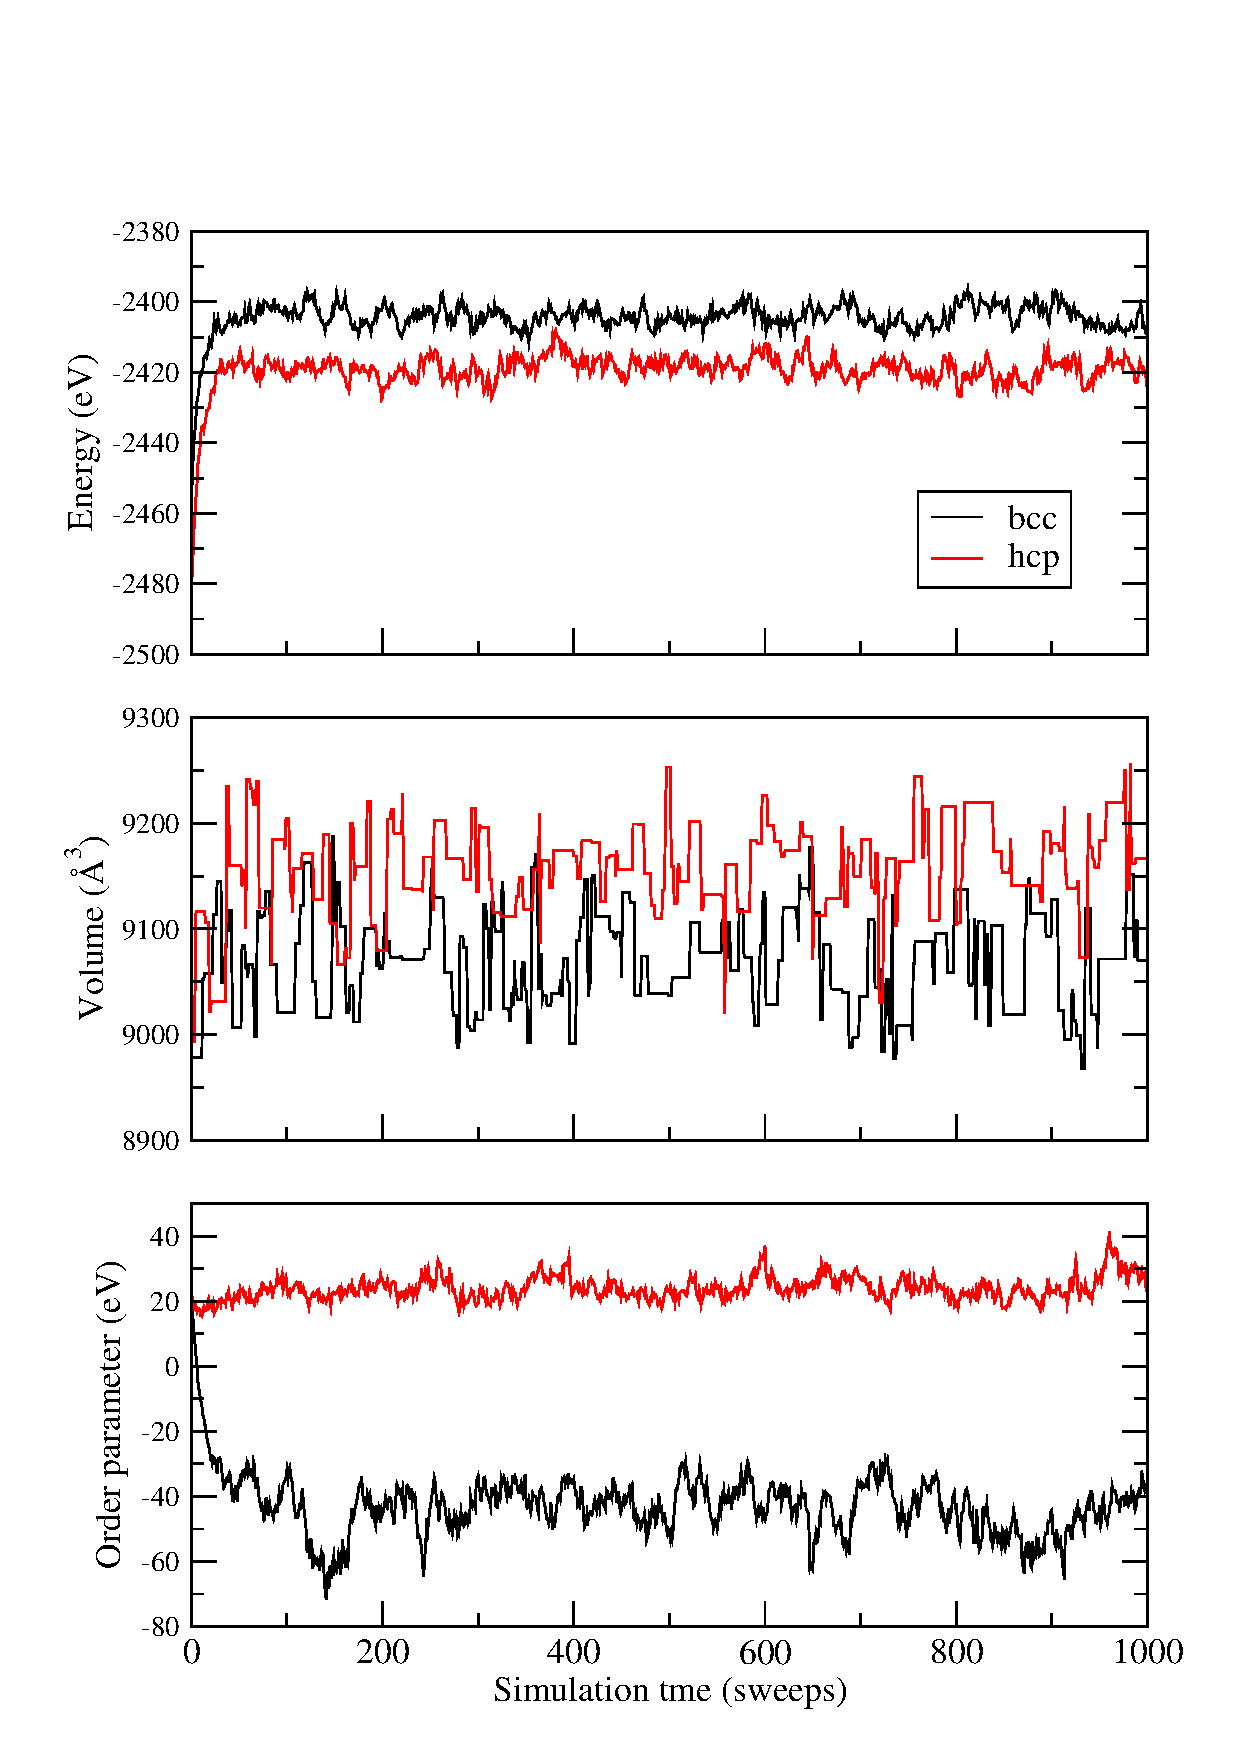
\includegraphics[width=\textwidth]{preliminary_results}
\caption
{Plots of the system's energy (top panel), volume (middle panel) and order parameter (bottom panel) vs. simulation time for the preliminary simulations.
The black curves correspond to the bcc preliminary simulation, while the red curves correspond to the hcp simulation.}
\label{fig:preliminary_results}
\end{figure}

\section{Weight function generation}\label{sec:example_generation}
The preliminary simulations have provided us with appropriate values for the maximum particle and volume move sizes, an estimate for
the equilibration time, and an appropriate order-parameter range. With this information we can
now begin LSMC simulations. The first such simulation is to generate the weight function. The directory
\texttt{weight\_function\_generation} corresponds to this simulation. We use artificial dynamics to generate the weight function. 
Furthermore we use \texttt{monteswitch\_mpi} to perform a parallelised calculation. Specifically we used 4 threads on a 4-core desktop machine. 
The following command was used to invoke the simulation (from within the \texttt{Examples/weight\_function\_generation} within the \emph{monteswitch} 
package itself) on our desktop machine:
\begin{verbatim}
$ mpiexec -n 4 ../../../monteswitch_mpi -new
\end{verbatim}
The appropriate command may be different for the user's platform.

\subsection{The \texttt{params\_in} file}
The salient features of the \texttt{params\_in} files for this simulation are as follows:
\begin{itemize}
\item \textbf{init\_lattice} is set to 1, which means that the simulation is initialised in the bcc phase. However, the choice of initial phase is 
  unimportant since both phases will be explored during the simulation.
\item \textbf{M\_grid\_size}, \textbf{M\_grid\_min} and \textbf{M\_grid\_max} define the macrostates. We set \textbf{M\_grid\_min} and \textbf{M\_grid\_max}
  to -82 and 48, which corresponds to the appropriate range determined from our preliminary simulations. 
  Furthermore, we set \textbf{M\_grid\_size} to 100: the order-parameter range will be divided into
  100 macrostates. The choice of 100 is based upon our previous experience, and may not be appropriate for all systems. 
  Recall that if the number of macrostates is too high, then the weight function will take longer to generate. On the other hand if the number of macrostates
  is too low, then the system is unable to explore the whole range of order-parameter space in a reasonable simulation time -- regardless
  of the weight function. This occurs because the order-parameter grid is too coarse to be able to guide the system over any free energy barriers.
  (See Section \ref{sec:multicanonical_LSMC}).
\item \textbf{enable\_multicanonical} is set to \texttt{T}, which means that the continually updated weight function is used to bias the dynamics of the system.
  This is actually unnecessary here since we elect to use artificial dynamics to guide the system through order-parameter space. Artificial dynamics would
  work well with canonical sampling. However, using multicanonical sampling in theory should result in the system transitioning between adjacent macrostates 
  more easily, speeding up the exploration of order-parameter space slightly.
\item \textbf{enable\_lattice\_moves} is set to \texttt{T}: the system can explore both phases using lattice moves.
\item \textbf{part\_step} and \textbf{vol\_step} are informed by our preliminary simulations
\item \textbf{stop\_sweeps} is set to 160000. Note that since we are using 4 MPI threads, each thread will perform 40000 sweeps.
\item \textbf{output\_file\_period} is set to 250. We do this mainly to avoid creating massive output files. At this point we do not need to know 
  information regarding the time-evolution of the system during the simulation on the scale of less than 250 sweeps, given that the equilibration time is
  $\lesssim 200$ sweeps. Note that since we are using \texttt{monteswitch\_mpi} there is one output file for each thread; for each thread $n$, every 
  250 sweeps information is output to the file \texttt{data\_n}.
\item \textbf{output\_stdout\_period} is set to -1, which suppresses all output to stdout. This is normally desirable for MPI simulations, since each thread 
  will itself output to stdout every \textbf{output\_stdout\_period} sweeps, which can result in an overwhelming amount of (and confusing) information to 
  stdout. 
  Furthermore, for long simulations we have no interest in watching the simulation variables during the running of the simulation -- which is the primary
  purpose of the simulation outputting information to stdout. Instead we let the simulation run, say, overnight, and extract the information we require
  from the \texttt{data} and \texttt{state} files once it is completed -- no information is output to stdout which cannot be obtained from these files.
\item \textbf{checkpoint\_period} is set to 2000; every 2000 sweeps the state of each MPI thread $n$ is output to the file \texttt{state\_n}.
\item \textbf{update\_eta} is set to \texttt{T}, which means that the simulation periodically updates/generates the weight function
\item \textbf{update\_eta\_sweeps} is set to 2000; we update the weight function (in this case using the shooting method, see below) every 2000 
  sweeps.
\item \textbf{update\_eta\_method} is set to \verb|"shooting"|, which means that the weight function is determined from the transition matrix via the 
  shooting method (see Section \ref{sec:transition_matrix}). This obviously requires the matrix \textbf{trans} to be updated during the simulation. 
  Accordingly we set \textbf{update\_trans} to \texttt{T}, otherwise
  the transition matrix is not updated during the simulation and updating the weight function using the shooting method will not work.
\item \textbf{enable\_barriers} is set to \texttt{T} since we wish to use artificial dynamics to force the system to quickly explore the whole of
  order-parameter space. Specifically, we elect to have the system sweep through the macrostates sequentially, proceeding first towards macrostate 1, 
  then from there to macrostate 100, thenback to macrostate 1, etc. Accordingly we set \textbf{barrier\_dynamics} to \verb|"pong_down"|.
\item \textbf{lock\_moves} controls how long the system is `locked' into each macrostate by the `macrostate barriers' during artificial dynamics, 
  before the `next' macrostate is opened to the system. This period should be long enough that the system has enough time to equilibrate locally within the 
  macrostate, but not so long that the system never ends up exploring all macrostates during the simulation. Our choice of 38400 (=100 sweeps) seems 
  to do the job. Note that while the equilibration time in our preliminary simulations was $\lesssim 200$ sweeps, the time to equilibrate locally
  \emph{within one macrostate} is expected to be far shorter. Furthermore, the time spent in each macrostate will actually be longer than 
  \textbf{lock\_moves}: \textbf{lock\_moves} is the number of moves before a new macrostate becomes available to the system; the system still must 
  move into that new macrostate from the `old' macrostate by its own accord. As expected, it takes longer for the system to move from old macrostates 
  into new macrostates if the free energy difference difference between the macrostates is high.
\end{itemize}

\subsection{Results}
At the completion of the simulation the file \texttt{state} (not \texttt{state\_0}, \texttt{state\_1}, \texttt{state\_2} or \texttt{state\_3}) 
contains the final results of the simulation --
pooled from all 4 MPI threads. We are obviously interested in the weight function. This can be obtained from the \texttt{state} file using 
\texttt{monteswitch\_post}.
After the following command (invoked from within the \texttt{weight\_function\_generation} directory), the file \texttt{wf.dat} contains the weight 
function vs. order parameter:
\begin{verbatim}
$ ../../../monteswitch_post -extract_wf > wf.dat
\end{verbatim}
\texttt{wf.dat} is plotted in Fig. \ref{fig:generation_results}. Note that the weight function is a smooth curve with two minima separated by a high peak 
near $M=0$. This is the expected form for a weight function. If the curve were not smooth, or was constant for large regions of order-parameter space, then 
it is probable that the weight function has not properly been generated. This is perhaps an indication that more time is needed to generate a 
reasonable weight function. One possible solution is to continue the simulation with \texttt{monteswitch\_mpi} using the \texttt{-resume} flag, e.g.
\begin{verbatim}
$ mpiexec -n 4 ../../../monteswitch_mpi -resume
\end{verbatim}

Of course, just because the weight function has the form described above does not guarantee that it is good. Recall that the ideal weight function
leads to the whole considered range of order-parameter space being sampled uniformly. A weight function with the form described above could easily lead to
certain regions of order-parameter space being significantly over- or under-sampled. In principle this is not a problem because the final results -- given
a long enough production simulation -- do not depend on the specific weight function used. However the quality of the weight function does determine how 
efficiently phase space is explored in the production simulation. Using a weight function of high quality samples order-parameter space almost uniformly, resulting
in many accepted lattice switches, and both phases being explored over short timescales. On the other hand if a low-quality weight function is used then the
system would spend more time in certain regions of order-parameter space than others, and the time between lattice-switches would be less. Hence it is prudent
to perform a short simulation using the weight function to verify that it is of good quality. We do this below.

\begin{figure}
\centering
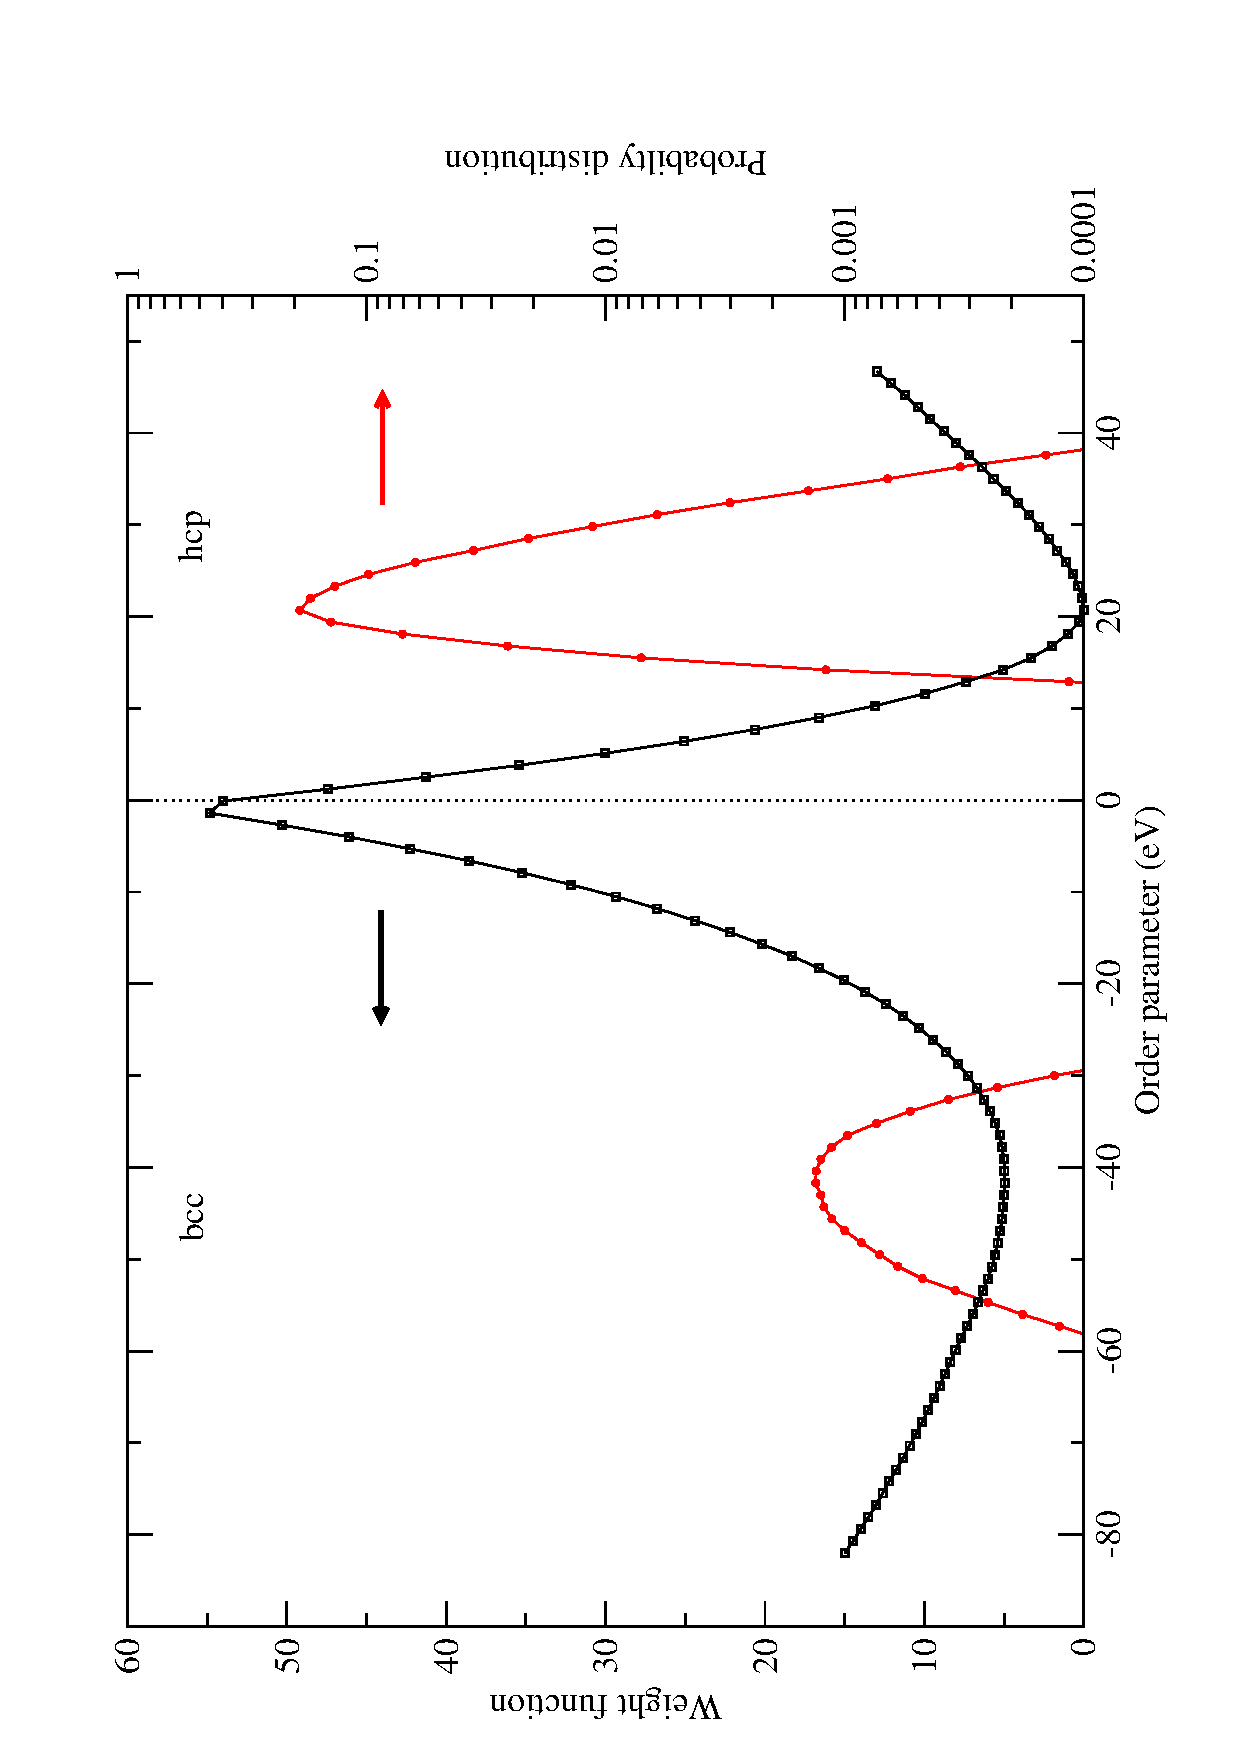
\includegraphics[height=\textwidth,angle=270]{generation_results}
\caption
{Results of the weight function generation simulation. The black curve and square symbols correspond to the weight function, while the red curve and circles 
corresponds to the probability distribution inferred from the weight function (as described in the main text). Note that the left vertical axis corresponds to the 
weight function while the right axis corresponds to the probability distribution -- as indicated by the arrows. The regions of order-parameter space 
corresponding to bcc and hcp are indicated.}
\label{fig:generation_results}
\end{figure}

\subsection{Checking the chosen order-parameter range}\label{section:double_check}
The ideal weight function is related to the canonical macrostate probability distribution via Eqn. \eqref{ideal_wf}. Using this equation one can obtain the
probability distribution from the weight function. Of course, this will only be the `true' probability distribution if the weight function is ideal, which it
will not be near given the short length of our weight function generation simulation. Nevertheless we can obtain an \emph{approximate} probability distribution 
from our weight function using Eqn. \eqref{ideal_wf}. This is useful for checking that our chosen order-parameter range is appropriate. 
We use the following command to obtain the probability distribution from the weight function, outputting it to the file \texttt{prob.dat}:
\begin{verbatim}
$ awk 'FNR==NR {sum=sum+exp(-$2); next} {print $1,exp(-$2)/sum}'
wf.dat wf.dat > prob.dat
\end{verbatim}
(Note that the appearance of \texttt{wf.dat} twice in the above command is deliberate). \texttt{prob.dat} is plotted in Fig. \ref{fig:generation_results}.
Note that the probability distribution has two peaks in order-parameter space, each corresponding to one phase. Now, the order-parameter
range is suitable only if the probability distribution is effectively zero at the maximum and minimum order parameters considered. If this is not the
case, then some states which are significantly likely at equilibrium would be `cut out' of the calculation of thermodynamic quantities, because moves which
take the system outside the order-parameter range are automatically rejected. Fortunately here the probability distribution decays to essentially zero within 
the considered range as required. If this were not the case then we would have to re-run the weight function generation simulation using a larger 
order-parameter range.


\subsection{Estimating $\Delta G$ from the weight function}
With the aforementioned probabilty distribution one can obtain an estimate of the free energy difference between the phases. Recall that the
free energy difference $\Delta G$ is related to the time spent in each phase via Eqn. \eqref{DeltaF_stat_mech}, where $p_2$ and $p_1$ are the (canonical) 
probabilities that the system is in phase 1 and 2 respectively. 
$p_1$ and $p_2$ can be deduced by integrating over the corresponding peaks in the probability distribution in \texttt{prob.dat}. 
Noting that the peak in the negative region of order-parameter space corresponds to bcc, and that the peak in the positive region corresponds to hcp, it
can be seen that the command applies Eqn. \eqref{DeltaF_stat_mech} to obtain the free energy difference indirectly from the weight function:
\begin{verbatim}
$ awk '{if($1<0){sum1=sum1+$2}; if($1>0){sum2=sum2+$2}} END{print
-log(sum1/sum2)/9.403 }' prob.dat
\end{verbatim}
Recall that 9.403 is the value of $\beta$ we are considering.
The intensive value of $\Delta G$ is obtained by dividing by the extensive value by the number of atoms in the system, which in this case is 384:
\begin{verbatim}
$ awk '{if($1<0){sum1=sum1+$2}; if($1>0){sum2=sum2+$2}} END{print
-log(sum1/sum2)/(9.403*384) }' prob.dat
\end{verbatim}
This command gives $\Delta G$ to be 0.00113081eV per particle, which corresponds to the hcp phase being very slightly more favoured than
the bcc phase (since in \emph{monteswitch} $\Delta G$ is the free energy of phase 1, which is bcc here, relative to phase 2, which is hcp here). 
We will compare this value with the `true' value we obtain for $\Delta G$ later.

We emphasise that this method provides only an estimate for $\Delta G$. Crucially, unlike $\Delta G$ obtained from the forthcoming production
simulation, the method does not provide an uncertainty for $\Delta G$. Hence one should not rely upon this method
for accurate results, though the method could be used, e.g., to quickly determine estimates for $\Delta G$ over a wide range of 
$T$, perhaps with the aim of deducing the approximate position of the transition temperature (where $\Delta G=0$).


\subsection{Using other weight function generation methods}
In the above example we used the transition-matrix method in conjunction with artificial dynamics to generate the weight function. This method gives a 
reasonable weight function very quickly. However, \emph{monteswitch} supports other methods for generating weight functions. These were described in 
Section \ref{sec:weight_generation}, namely the visited states method, and the transition-matrix method in conjunction with \emph{natural} dynamics.
The variables in \texttt{params\_in} required to implement each of the aforementioned methods within \emph{monteswitch} are shown in Table 
\ref{table:wf_gen_variables}. Recall that for the transition-matrix method with artificial dynamics there are two possibilities: evolving the
macrostate barriers randomly or systematically.
Guidelines are also provided in the table regarding values for \textbf{update\_eta\_sweeps} and
\textbf{lock\_moves} for each method. The reasoning behind these guidelines is as follows. 
For the visited states method, \textbf{update\_eta\_sweeps} corresponds to the block size mentioned in
Section \ref{sec:visited_states}. This should be long enough such that a block is representative of a `long' multicanonical simulation with the 
current weight function. Furthermore, the closer to the ideal weight function one wishes to get, the longer the blocks should be.
For the transition-matrix method, if multicanonical sampling is used, then one may as well update the weight function `continuously'. In this case
the weight function used always reflects all the information gathered so far during the weight function generation simulation, thus enabling the
system to explore order parameter space as widely as possible in as short a simulation time as possible. Regarding the choice of
\textbf{lock\_moves}, see the discussion in Section \ref{sec:example_generation}.

\begin{landscape}
\begin{table}\label{table:wf_gen_variables}
\begin{center}
\begin{tabular}{l p{4cm} p{2cm} p{6cm}}
Control variable                   & VS                & TM-ND                & TM-AD \\
\hline 
\textbf{enable\_multicanonical}    & \texttt{T}        &   \texttt{T}         &  \texttt{F} or \texttt{T}   \\
\textbf{update\_eta}               & \texttt{T}        &   \texttt{T}         &  \texttt{T}                 \\
\textbf{update\_eta\_sweeps}       & $\gg$ multicanonical correlation time (in sweeps)  & $\sim 1$ &   $\sim 1$ if \textbf{enable\_multicanonical}=\texttt{T}; 
   $\leq$ \textbf{stop\_sweeps} if \textbf{enable\_multicanonical}=\texttt{F} \\
\textbf{update\_trans}             & N/A               &   \texttt{T}         &  \texttt{T}                 \\
\textbf{update\_eta\_method}       & \texttt{"VS"}       &   \texttt{"shooting"}  &  \texttt{"shooting"}     \\
\textbf{enable\_barriers}          & \texttt{F}        &   \texttt{F}         &  \texttt{T}                 \\
\textbf{barrier\_dynamics}         & N/A               &   N/A                &  \texttt{"random"} for random macrostate barrier evolution;
    \texttt{pong\_up} or \texttt{pong\_down} for systematic evolution  \\
\textbf{lock\_moves}               & N/A               &   N/A                &  $\gtrsim$ time to equilibrate \emph{within a macrostate} (in moves) \\
\end{tabular}
\end{center}
\caption{Values for variables in \texttt{params\_in} or \texttt{state} required to implement various weight function generation methods.
`VS' refers to the visited states method; `TM-D' refers to the transition-matrix method with natural dynamics; `TM-AD' refers to the
transition-matrix method with artificial dynamics. (See Section \ref{sec:weight_generation} for descriptions of these methods). `N/A' 
signifies that the variable is not used in the method, and hence its value is unimportant}
\end{table}
\end{landscape}


\section{Weight function verification}
Assuming that we have a good weight function, one thing remains which is useful to know before we perform our production simulation: the correlation time 
for the multicanonical simulation using this weight function.
\footnote{Presumably one could make the multicanonical simulation more efficient by optimising the maximum particle and volume move step sizes used in the 
multicanonical simulation, and not simply using the same values as for the canonical simulation. We have never done this, though it is something worth 
investigating.}
Recall that we obtained an estimate for the equilibration time earlier, and that it was $\lesssim 200$ sweeps. However, this applies only to 
a one-phase canonical simulation. As we will see in a moment, the correlation time in the two-phase multicanonical LSMC simulation is much longer. 
We need to know the multicanonical correlation time because it determines how large the blocks should be for block averaging to calculate thermodynamic quantities,
in particular the free energy difference. To determine this correlation time we perform a short multicanonical simulation using the weight function. This 
simulation also acts to check verify that the weight function is indeed sensible, i.e., that it leads to the entire range of order-parameter space being 
explored approximately uniformly.

The directory \texttt{weight\_function\_verification} corresponds to the weight function verification simulation.
Recall that we can `resume' a simulation whose variables are stored in the \texttt{state} file by invoking \texttt{monteswitch} with the 
\texttt{-resume} argument. Furthermore
we can resume a simulation from \texttt{state} but with all counter variables reset to zero by invoking the \texttt{-reset} argument. With this in mind, we
use the \texttt{state} file from our weight function generation simulation as a starting point. This file contains the weight function we wish to verify. 
We will modify this file to suit our needs, and then run the simulation using the command (from within the directory \texttt{weight\_function\_verification})
\begin{verbatim}
$ ../../../monteswitch -reset
\end{verbatim}
Note that the file \texttt{state\_start} in the directory \texttt{weight\_function\_verification} contains the \texttt{state} file from the directory 
\texttt{weight\_function\_generation} after it has been modified for the weight function verification simulation; and the file \texttt{state} in the 
directory \texttt{weight\_function\_verification} corresponds to the output of the weight function verification simulation.

\subsection{Creating the input \texttt{state} file}
The modifications to the \texttt{state} file before the weight function verification simulation is run can be seen by invoking the following command
in the \texttt{weight\_function\_verification} directory:
\begin{verbatim}
$ diff state_start ../weight_function_generation/state
\end{verbatim}
The key changes are as follows:
\begin{itemize}
\item We have changed \textbf{stop\_sweeps} to be 10000, which corresponds to a short simulation.
\item We have set \textbf{update\_eta} to \texttt{F}, so that the weight function is fixed throughout the simulation.
\item We have set \textbf{enable\_barriers} to \texttt{F}, since we want `natural' dynamics for the weight function verification simulation.
\item We have set \textbf{output\_file\_period} to 10 so we have high-resolution information about how order-parameter space is explored.
\item We have set \textbf{output\_stdout\_period} to 10 so we can view the progress of the simulation: information is output to stdout every 10 sweeps.
\end{itemize}

\subsection{Results}
After the simulation is complete we can use \texttt{data} to generate a plot of the order parameter vs. time in the same manner as for the
preliminary simulations:
\begin{verbatim}
$ grep 'M:' data | awk '{print $2,$3}' > M_vs_t.dat
\end{verbatim}
\texttt{M\_vs\_t.dat} is plotted in Fig. \ref{fig:verification_results} -- see the results for the first 10000 sweeps. From the figure it can be seen
that the entire range of order-parameter space was explored within the simulation. However, a 10000-sweep simulation in this case is too short to
estimate the correlation time: within the 10000 sweeps the system only makes one significant transition between the phases, from hcp to bcc. For 
this reason we continued the simulation for another 10000 sweeps by invoking the command
\begin{verbatim}
$ ../../../monteswitch -resume
\end{verbatim}
Hence the output files \texttt{state} and \texttt{data}, and \texttt{M\_vs\_t.dat} in the \texttt{weight\_function\_verification} directory correspond
to 20000 sweeps, not 10000 sweeps. (A copy of the output \texttt{state} file after the first-10000 sweep simulation can be found in the file 
\texttt{state\_after\_10000\_sweeps}). As can be seen from the figure, there are additional transitions between the phases in the second 10000 sweeps. 
Hence the correlation time -- which in this case involves both phases being explored -- is $\sim 10000$ sweeps. The 
block size we use in the forthcoming production simulation must be much greater than this. Note that after the production run one can 
retrospectively check that the block size was appropriate. We will do this later. Furthermore, one could use the informtion contained in the \texttt{data} 
file output by the production simulation to perform block averaging for a variety of block sizes, though we do not explain how to do this here.

It is instructive to plot how often each macrostate was visited during the weight function verification simulation. \texttt{monteswitch\_post}
provides an easy means of doing this: the following command creates a file \texttt{counts\_vs\_M.dat}, which is a plot of the order 
parameter for each macrostate (the lower bound for the order parameter range covered by the macrostate) vs. the number of times the macrostate 
was visited during the simulation:
\begin{verbatim}
$ ../../../monteswitch_post -extract_M_counts | awk '{print 
$1,$2+$3}' > counts_vs_M.dat
\end{verbatim}
\texttt{counts\_vs\_M.dat} is plotted in the inset of Fig. \ref{fig:verification_results}. From this we see that all macrostates were visited.
It is conspicuous that the histogram is not flat. We would in fact be very lucky to get a flat histogram, even with the ideal weight function, given 
that we only performed 20000 sweeps -- which is the order of the correlation time.

\begin{figure}
\centering
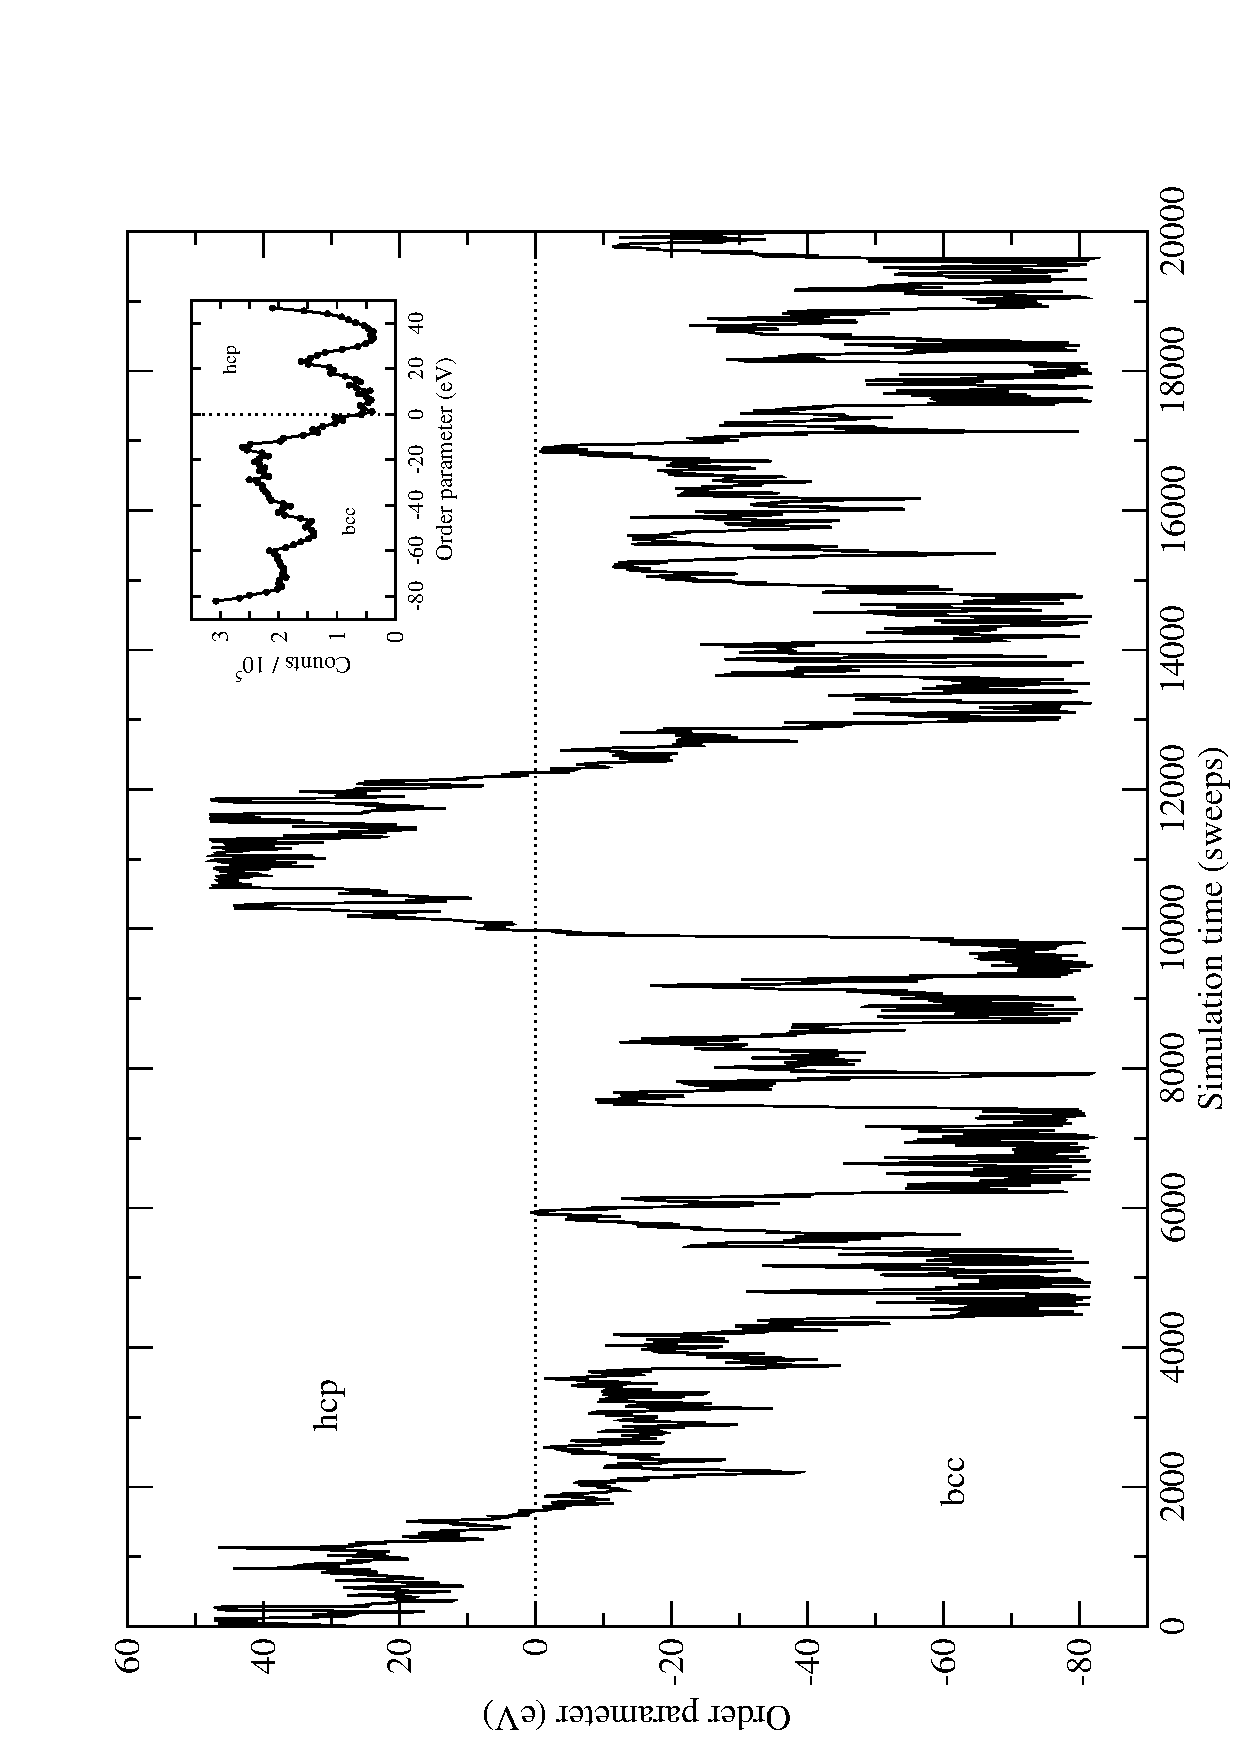
\includegraphics[height=\textwidth,angle=270]{verification_results}
\caption
{Plot of the order parameter vs. simulation time for the weight function verification simulation. The regions of order-parameter space 
corresponding to bcc and hcp are indicated. The inset is a histogram of how often each macrostate (identified by its order parameter as described
in the main text) was visited during the simulation.}
\label{fig:verification_results}
\end{figure}


\section{Production simulation}
We are now finally ready to perform the production simulation. The corresponding directory is \texttt{production\_simulation}.
As with the weight function verification simulation, we use the \texttt{state} file output from the weight function generation simulation as 
the starting point for the production simulation. We will modify this file to suit our needs, and then run the simulation, using four MPI threads with 
\texttt{monteswitch\_mpi}, using the command (invoked from within the \texttt{production\_simulation} directory)
\begin{verbatim}
$ mpiexec -n 4 ../../../monteswitch_mpi -reset
\end{verbatim}
Note that again we have used the \texttt{-reset} flag to reset the counter variables at initialisation.

\subsection{Creating the input \texttt{state} file}
The modifications to the state file can be seen by invoking the following command in the \texttt{production\_simulation} directory:
\begin{verbatim}
$ diff state_start ../weight_function_generation/state
\end{verbatim}
The key changes are as follows:
\begin{itemize}
\item We have changed \textbf{stop\_sweeps} to be 700000, which corresponds to 175000 sweeps to be performed for each MPI thread.
\item We have set \textbf{equil\_sweeps} to 20000, which is larger than the correlation time we determined via the weight function verification
simulation.
\item We have set \textbf{update\_eta} to \texttt{F} so that the weight function is fixed throughout the simulation.
\item We have set \textbf{enable\_barriers} to \texttt{F} since we want 'natural' dynamics for the production simulation.
\item \textbf{calc\_equil\_properties} is set to \texttt{T}. This is required for the simulation to calculate thermodynamic quantities (in particular
$\Delta G$, and the enthalpy and volume of each phase) and their uncertainties using block averaging.
\item \textbf{block\_sweeps}, the number of sweeps which constitute a block in the block averaging is set to 155000, which is far larger than the 
correlation time of $\sim 10000$ sweeps determined in the weight function verification simulation. Note that, since each MPI thread performs 
175000 sweeps, and since each thread will be given 20000 sweeps to equilibrate -- during which time the states visited by the system are not 
used in block averaging - setting the block size to 155000 sweeps corresponds to each MPI thread performing exactly 1 block. Hence the 
simulation in total considers 4 blocks.
\end{itemize}

\subsection{Results}
At the completion of the simulation the \texttt{state} file contains the thermodynamic quantities evaluated using block averaging. It is these quantities we
are interested in, especially $\Delta G$. The variables \textbf{equil\_DeltaF} and \textbf{sigma\_equil\_DeltaF} in \texttt{state} contain 
$\Delta G$ and its uncertainty evaluated using block averaging. The following command extracts these variables from the \texttt{state} file:
\begin{verbatim}
$ grep -E '( equil_DeltaF| sigma_equil_DeltaF)' state
\end{verbatim} 
Recall that all quantities in the \texttt{state} file are extensive. To get the intensive values we must divide them by the number of atoms in the system, 
which in this case is 384. Hence the following command gives the intensive free energy difference between the phases:
\begin{verbatim}
$ grep -E '( equil_DeltaF| sigma_equil_DeltaF)' state | awk
'{print $1,$2/384}'
\end{verbatim}
Using this we find that $\Delta G$ is 0.00104(2)eV per particle, which implies that hcp is slightly favoured over bcc at this $T$ and $P$.
Note that this agrees favourably with the $\Delta G$ we obtained from the weight function earlier, namely 0.00113 eV per particle.
However, note that $\Delta G$ is $\sim$1 meV per particle, which is very small. Thus $T=$1233K is very close to the zero-pressure bcc--hcp transition
temperature: we are in agreement with Ref. \cite{Mendelev_2007}.

We will now show that we are also in agreement with Ref. \cite{Mendelev_2007} with regards to $\Delta H_{\text{hcp$\to$bcc}}$ and 
$\Delta V_{\text{hcp$\to$bcc}}/V_{\text{bcc}}$. Using similar commands to the above, one can extract the volume and enthalpy per atom for each phase
evaluated using block averaging, as well as their associated uncertainties:
\begin{verbatim}
$ grep -E '( equil_V_1| sigma_equil_V_1)' state | awk '{print $1,
 $2/384}'
\end{verbatim}
gives the volume per atom for phase 1;
\begin{verbatim}
$ grep -E '( equil_V_2| sigma_equil_V_2)' state | awk '{print $1,
  $2/384}'
\end{verbatim}
gives the volume per atom for phase 2;
\begin{verbatim}
$ grep -E '( equil_H_1| sigma_equil_H_1)' state | awk '{print $1,
 $2/384}'
\end{verbatim}
gives the enthalpy per atom for phase 1; and
\begin{verbatim}
$ grep -E '( equil_H_2| sigma_equil_H_2)' state | awk '{print $1,
 $2/384}'
\end{verbatim}
gives the enthalpy per atom for phase 2. Using these quantities one can calculate $\Delta H_{\text{hcp$\to$bcc}}$ and $\Delta V_{\text{hcp$\to$bcc}}/V_{\text{bcc}}$,
which are presented in Table \ref{table:production_results} alongside the results of Ref. \cite{Mendelev_2007}. As can be seen from the table
the quantities obtained from the production simulation are in excellent agreement with those of Ref. \cite{Mendelev_2007}. Of course, it is unnecessary 
to use an LSMC simulation to extract such one-phase thermodynamic quantities; a pair of conventional Monte Carlo simulations will do the job more 
efficiently. Here the quantities are somewhat of a by-product of the LSMC simulation, which \emph{is} however required to calculate the \emph{two-phase}
quantity $\Delta G$.

\begin{table}\label{table:production_results}
\begin{center}
\begin{tabular}{l  l  l }
Quantity                                  &  \emph{monteswitch}      & Ref. \cite{Mendelev_2007} \\
                                                        \hline
$\Delta H_{\text{hcp$\to$bcc}}$ (eV)                 & 0.0394(2)                & 0.039                     \\
$\Delta V_{\text{hcp$\to$bcc}}/V_{\text{bcc}}$ (\%)          & -0.812(7)                & -0.8                      \\
\end{tabular}
\caption{Thermodynamics quantities obtained from the production simulation, and analogous quantities obtained in Ref.  \cite{Mendelev_2007}. Note that
the quoted $\Delta H_{\text{hcp$\to$bcc}}$ is intensive, i.e., `per particle'.}
\end{center}
\end{table}


\subsection{Final checks}
Once the production simulation is complete it is prudent to perform some checks to ensure that it has gone as expected, and hence that the values for the
thermodynamic quantities obtained from the simulation are meaningful. Comparing the thermodynamic quantities obtained from the simulation 
to `known' values, as was done above, is an excellent consistency check. However this will not always be possible. A less obvious check to perform is 
as follows.
%
The free energy difference for a block is given by Eqn. \eqref{DeltaF_stat_mech}, where in this case $t_1$ and $t_2$ are the number of moves which the 
system spent in phase 1 and phase 2 respectively during the block. Note that this equation presupposes that both phases are explored during the block. 
Now, in evaluating $\Delta G$, \emph{monteswitch} only considers blocks during which both phases are explored. This notwithstanding, one should check that
the block size is significantly larger than the time it typically takes the system to explore the whole of order-parameter space -- which in practice
is an equivalent condition to both phases being thoroughly explored during each block. To do this we plot the order parameter vs. simulation time for each
MPI thread using the following commands:
\begin{verbatim}
$ grep 'M:' data_0 | awk '{print $2,$3}' > M_vs_t_0.dat
$ grep 'M:' data_1 | awk '{print $2,$3}' > M_vs_t_1.dat
$ grep 'M:' data_2 | awk '{print $2,$3}' > M_vs_t_2.dat
$ grep 'M:' data_3 | awk '{print $2,$3}' > M_vs_t_3.dat
\end{verbatim}
where \texttt{M\_vs\_t\_n.dat} is a plot of order parameter vs. simulation time for thread $n$. These plots are shown in Fig. \ref{fig:production_results}.
As can be seen from the figure, for each thread the system traverses the entire range of order-parameter space often within the block size (175000 
sweeps), as required.
%
Of course, the aim of the weight function verification simulation was to ensure that this would happen: in that simulation we deduced the correlation time,
and used that to inform our choice of block size. Still, it is good to double-check.

\begin{figure}
\centering
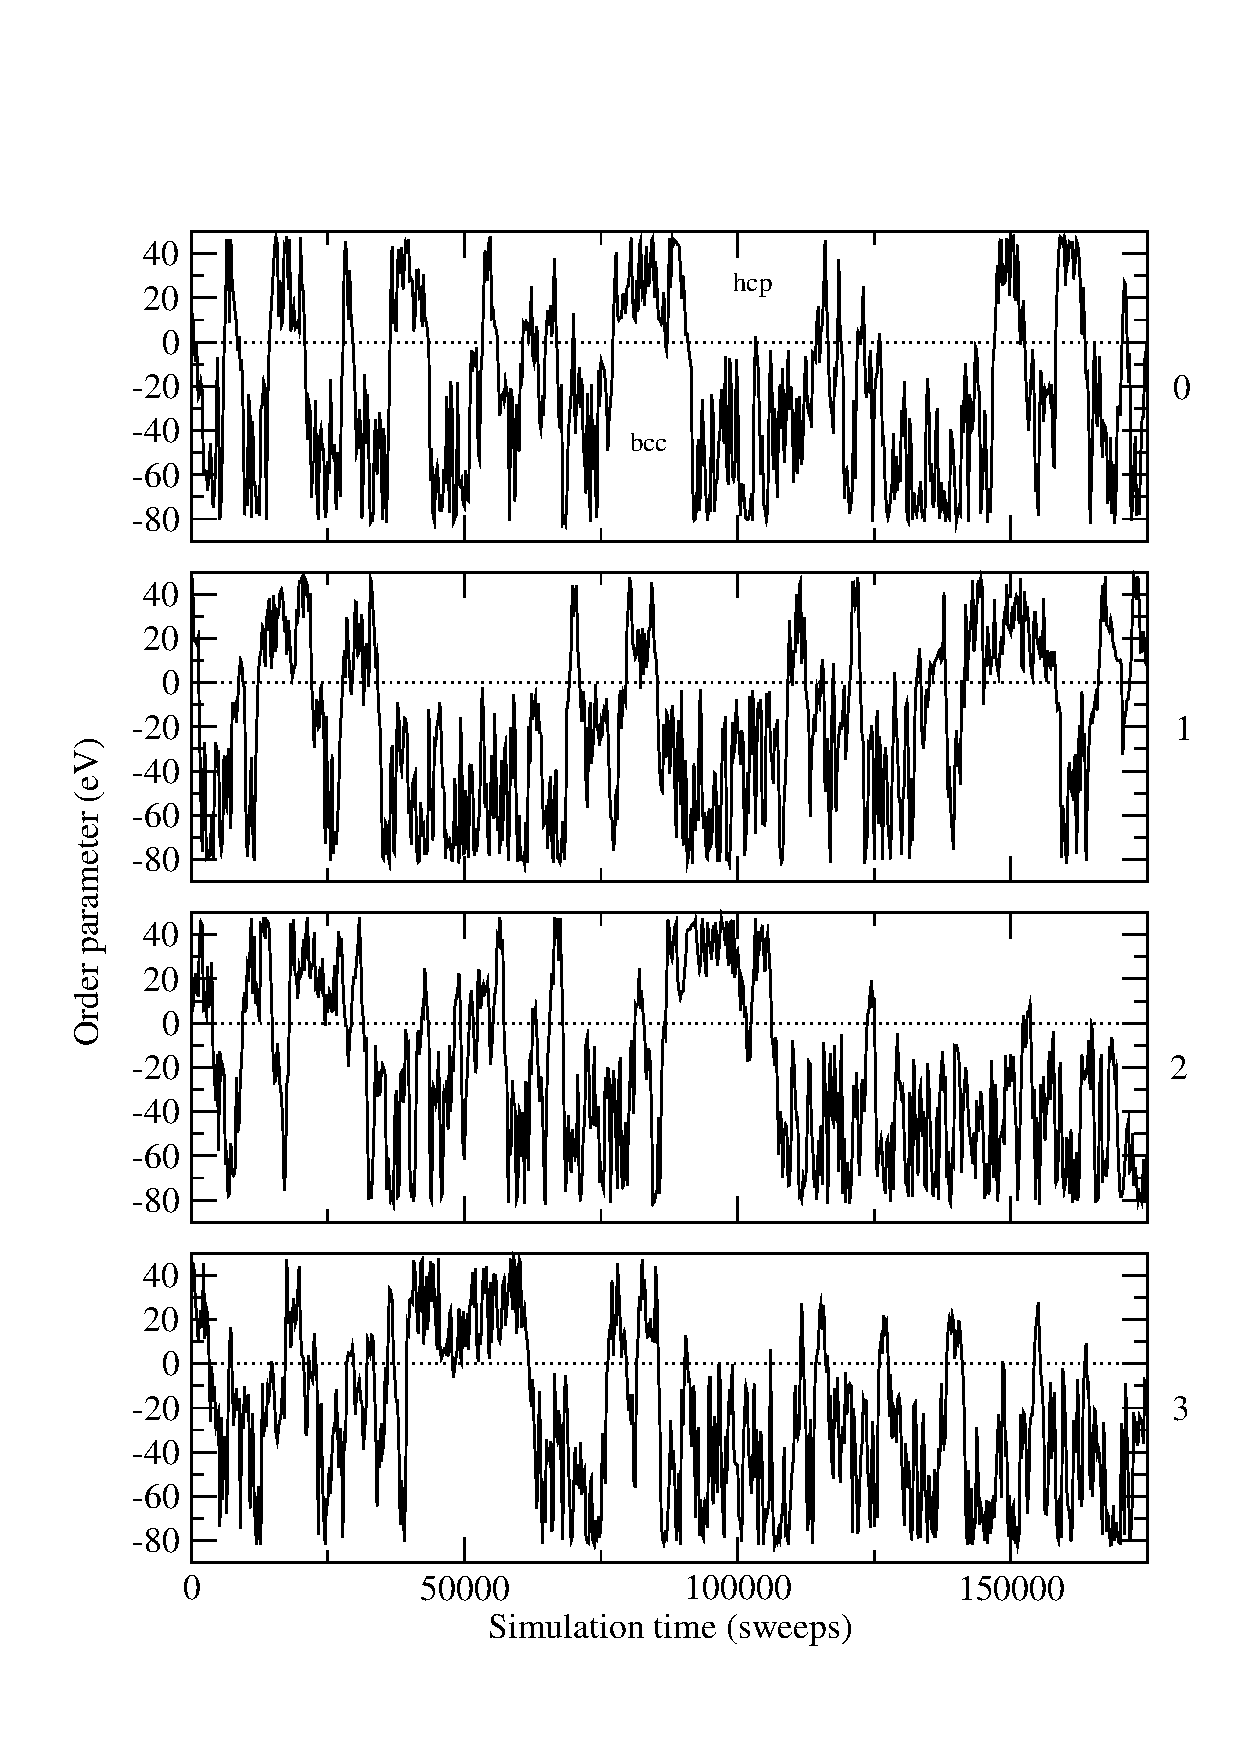
\includegraphics[width=\textwidth]{production_results}
\caption
{Plots of the order parameter vs. simulation time for each MPI thread for the production simulation. The number to the right of each panel corresponds
to the thread index. The regions of order-parameter space corresponding to bcc and hcp are indicated.}
\label{fig:production_results}
\end{figure}



%%%%%%%%%%%%%%%%%%%%%%%%%%%%%%%%%%%%%%%%%%%%%%%%%%%%%%%%%%%%%%%%%%%%%%%%%%%%%%%%%%%%%%%%%%%%%%%%%%%%%%%%%%
\chapter{Test cases}\label{chapter:tests}
The directory \texttt{Tests} contains a suite of test cases for the main programs in \emph{monteswitch}. Of course, these tests can also be used as
examples.

Each test can be executed by executing the \texttt{run.sh} shell script in the corresponding directory after copying the
appropriate \texttt{interactions.f95} file from \texttt{Interactions} to \texttt{interactions.f95}, and then compiling the
package (see Chapter \ref{chapter:preliminaries}). Note that the \texttt{run.sh} scripts assume that the main programs \texttt{monteswitch}
and \texttt{monteswitch\_mpi} are located in the same directory as the source code, which should be the case by default. Furthermore
the \texttt{run.sh} files may require some modification to suit your platform (see Chapter \ref{chapter:preliminaries}).


\section{Einstein crystal (\texttt{EC})}
In the Einstein crystal the energy of the system is given by
\begin{equation}
E=\sum_{i=1}^N\alpha u_i^2,
\end{equation}
where $u_i$ is the displacement of particle $i$ from its lattice site, $N$ denotes the number of particles in the system, and $\alpha$
is the free parameter of the model. The Einstein crystal is an excellent testing ground for \emph{monteswitch} because 
analytical results can be derived for this system. For instance, the free energy of the system is given by \cite{book:Frenkel}
\begin{equation}\label{EC_F}
F=-\frac{3N}{2\beta}\ln\biggl[\frac{\pi}{\alpha\beta}\biggr],
\end{equation}
where $\beta$ is the thermodynamic beta. Furthermore the mean-squared displacement of each particle is \cite{book:Frenkel}
\begin{equation}\label{EC_u2}
\langle u^2\rangle = \frac{3}{2\beta\alpha},
\end{equation}
and the mean energy of the system is
\begin{equation}\label{EC_E}
\langle E\rangle=\alpha N\langle u^2\rangle = \frac{3N}{2\beta}.
\end{equation}
Here we test \emph{monteswitch} against these analytical results. Our `phases' here are two Einstein crystals with different values
of $\alpha$. We denote the $\alpha$ pertaining to phase 1 as $\alpha_1$, and similarly for phase 2. Using Eqn. \eqref{EC_F},
the following expression for the free energy difference between the phases can be derived:
\begin{equation}\label{EC_DeltaF}
\Delta F\equiv F_1-F_2=\frac{3N}{2\beta}\ln\biggr[\frac{\alpha_1}{\alpha_2}\biggr].
\end{equation}
We use Eqns. \eqref{EC_u2}, \eqref{EC_E} and \eqref{EC_DeltaF} below.

The \texttt{interactions.f95} file corresponding to the Einstein crystal is \texttt{interactions\_EC.f95}. The Hamiltonian for 
each phase realised in \emph{monteswitch} in conjunction with \texttt{interactions\_EC.f95} is as described above, where 
note that the orign constitutes the lattice site \emph{for all particles}.
$\alpha_1$ and $\alpha_2$ are specified for new simulations via the input file \texttt{interactions\_in}. 
The format of this file is as follows. On the first line there are two tokens. The first token is an arbitrary \texttt{CHARACTER(LEN=20)} 
variable (we recommend: \texttt{alpha\_1=}). The second token is the value of $\alpha_1$ (stored internally as 
\textbf{alpha\_1}), which is of type \texttt{REAL}. The second line is similar, but for $\alpha_2$.


\subsection{\texttt{test\_EC\_1}}
This test calculates $\Delta F$, and $\langle u^2\rangle$ and $\langle E\rangle$ for each phase, for the case $\alpha_1=1$, $\alpha_2=2$,
$\beta=100$ and $N=1$. The test uses canonical (i.e., not multicanonical) sampling, and consists of 10,000,000 sweeps using 
\textbf{part\_step}=0.12.

The following checks should be performed at the completion of the test:
\begin{enumerate}
\item
$\Delta F$ should be $0.015\ln(1/2)=-0.0103972$: see the variables \textbf{equil\_DeltaF} and \textbf{sigma\_equil\_DeltaF} output
to stdout. 
\item
$\langle u^2\rangle$ should be 0.015 for phase 1 and 0.0075 for phase 2: see the 
variables \textbf{equil\_umsd\_1}, \textbf{sigma\_equil\_umsd\_1}, \textbf{equil\_umsd\_2} and \textbf{sigma\_equil\_umsd\_2} 
output to stdout.
\item
$\langle E\rangle$ should be 0.015 for both phases. Check that this is the case by examining the variables 
\textbf{equil\_H\_1}, \textbf{sigma\_equil\_H\_1}, \textbf{equil\_H\_2} and \textbf{sigma\_equil\_H\_2} in the output to stdout. 
\end{enumerate}


\subsection{\texttt{test\_EC\_1\_MPI}}
This test is the same as \texttt{test\_EC\_1}, except that an MPI simulation is run using 4 threads. In this case one should check that
1, 2 and 3 described in \texttt{test\_EC\_1} applies to the variables listed in the \texttt{state} file, as opposed to the
output to stdout. This test verifies that \texttt{monteswitch\_mpi} works correctly, especially that it correctly combines
the results from all threads before outputting the final results to \texttt{state}.


\subsection{\texttt{test\_EC\_2}}
This test is the same as \texttt{test\_EC\_1}, except that 10 simulations consisting of 1,000,000 sweeps each are performed
instead of one simulation of 10,000,000 sweeps, using both the \texttt{-resume} and \texttt{-new} arguments to the executable 
\texttt{monteswitch} instead of simply the \texttt{-new} argument. This test verifies that checkpointing works
correctly within \texttt{monteswitch}. Checks 1, 2 and 3 described in \texttt{test\_EC\_1} should be performed on the 
\texttt{state} file.


\subsection{\texttt{test\_EC\_2\_MPI}}
This test is the same as \texttt{test\_EC\_2}, except that 10 4-thread MPI simulations are performed. This test verifies 
that checkpointing works correctly for \texttt{monteswitch\_mpi}. Checks 1, 2 and 3 described in \texttt{test\_EC\_1} should be 
performed on the \texttt{state} file.


\subsection{\texttt{test\_EC\_3}}
This test calculates the thermodynamic quantities mentioned in \texttt{test\_EC\_1}, but uses multicanonical sampling instead
of canonical sampling, with a weight function generated using the visited states method. To elaborate, a weight function generation 
simulation is performed which consists of 10,000,000 sweeps. Then the \texttt{state} file is altered in preparation 
for the production simulation. Then the production simulation is performed, which consists of 10,000,000 sweeps.
Checks 1, 2 and 3 described in \texttt{test\_EC\_1} should be performed on the \texttt{state} file.


\subsection{\texttt{test\_EC\_4}}
This test is the same as \texttt{test\_EC\_3} except that the weight function is generated using the shooting method over
1,000,000 sweeps. Checks 1, 2 and 3 described in \texttt{test\_EC\_1} should be performed on the \texttt{state} file.


\subsection{\texttt{test\_EC\_4\_MPI}}
This test is the same as \texttt{test\_EC\_4}, but uses 2 MPI threads.
Checks 1, 2 and 3 described in \texttt{test\_EC\_1} should be performed on the \texttt{state} file.


\subsection{\texttt{test\_EC\_5}}
This test is the same as \texttt{test\_EC\_3}, however the weight function is generated using the shooting method 
in conjunction with `\texttt{"pong\_down"} artificial dynamics' and canonical sampling over 1,000,000 sweeps. 
Checks 1, 2 and 3 described in \texttt{test\_EC\_1} should be performed on the \texttt{state} file.
However, two further files are created during this test: \texttt{M\_vs\_t.dat} contains the value of the order parameter vs. 
simulation time, and \texttt{macro\_vs\_t.dat} contains the macrostate number vs. simulation time. Both plots should resemble a sawtooth.


\subsection{\texttt{test\_EC\_5\_MPI}}
This test is the same as \texttt{test\_EC\_5}, except that a 2-thread MPI simulation is performed, and `\texttt{"pong\_up"}
artificial dynamics' are used. In this case the additional files created by the test are \texttt{M\_vs\_t\_0.dat} and 
\texttt{macro\_vs\_t\_0.dat}, which pertain to MPI thread `0', and \texttt{M\_vs\_t\_1.dat} and \texttt{macro\_vs\_t\_1.dat},
which pertain to thread `1'. All files should have a sawtooth pattern.
Furthermore checks 1, 2 and 3 described in \texttt{test\_EC\_1} should be performed on the \texttt{state} file.


\subsection{\texttt{test\_EC\_6}}
This test is the same as \texttt{test\_EC\_5}, except that `\texttt{"random"} artificial dynamics' are used. The files 
\texttt{M\_vs\_t.dat} and \texttt{macro\_vs\_t.dat} in this case should resemble random walks.
Furthermore checks 1, 2 and 3 described in \texttt{test\_EC\_1} should be performed on the \texttt{state} file.


\subsection{\texttt{test\_EC\_7}}
This test is the same as \texttt{test\_EC\_5}, except that 10 simulations are performed (each consisting of 100,000
sweeps) instead of 1. This tests verifies that checkpointing works correctly with artificial dynamics.
Checks 1, 2 and 3 described in \texttt{test\_EC\_1} should be performed on the \texttt{state} file.


\subsection{\texttt{test\_EC\_7\_MPI}}
This test is similar to \texttt{test\_EC\_7}, except that 2 2-thread MPI simulations are performed such that the total
number of sweeps is 1,000,000.
Checks 1, 2 and 3 described in \texttt{test\_EC\_1} should be performed on the \texttt{state} file.


\subsection{\texttt{test\_EC\_8}}
This test is similar to \texttt{test\_EC\_1}, except that $N=4$ instead of 1.

The following checks should be performed at the completion of the test:
\begin{enumerate}
\item
$\Delta F$ should be $0.06\ln(1/2)=-0.0415888$:  see the variables \textbf{equil\_DeltaF} and \textbf{sigma\_equil\_DeltaF} output
to stdout.
\item
$\langle u^2\rangle$ should be 0.015 for phase 1 and 0.0075 for phase 2: see the 
variables \textbf{equil\_umsd\_1}, \textbf{sigma\_equil\_umsd\_1}, \textbf{equil\_umsd\_2} and \textbf{sigma\_equil\_umsd\_2} output to
stdout.
\item
$\langle E\rangle$ should be 0.06 for both phases. Check that this
is the case by examining the variables \textbf{equil\_H\_1}, \textbf{sigma\_equil\_H\_1}, \textbf{equil\_H\_2} and \textbf{sigma\_equil\_H\_2}
in the output to stdout
\end{enumerate}


\subsection{\texttt{test\_EC\_8\_MPI}}
This test is the same as \texttt{test\_EC\_8}, except that an MPI simulation is run using 4 threads.  In this case checks
1, 2 and 3 described in \texttt{test\_EC\_8} should apply to the variables listed in the \texttt{state} file -- as opposed to the output to
stdout. This test verifies that \texttt{monteswitch\_mpi} works correctly for systems containing multiple particles, especially that it correctly
combines the results from all threads before outputting the final results to \texttt{state}.


\subsection{\texttt{test\_EC\_9}}
This test is the same as \texttt{test\_EC\_8}, except that 10 simulations consisting of 1,000,000 sweeps each are performed
instead of one simulation of 10,000,000 sweeps, using both the \texttt{-resume} and \texttt{-new} arguments to the executable 
\texttt{monteswitch} instead of simply the \texttt{-new} argument. This test verifies that checkpointing works
correctly for systems containing multiple particles. Checks 1, 2 and 3 described in \texttt{test\_EC\_8} should be performed on the \texttt{state} file.


\subsection{\texttt{test\_EC\_9\_MPI}}
This test is the same as \texttt{test\_EC\_9}, except that 10 4-thread MPI simulations are performed. This test verifies 
that checkpointing works correctly for \texttt{monteswitch\_mpi} for systems containing multiple particles. 
Checks 1, 2 and 3 described in \texttt{test\_EC\_8} should be performed on the \texttt{state} file.


\section{NPT Einstein crystal (\texttt{EC\_NPT})}
The Einstein crystal model described in the previous section cannot be used to validate \emph{monteswitch} for the NPT ensemble: all of the test cases
described so far were for the NVT ensemble. Accordingly we consider here a generalisation of the Einstein crystal model suitable for testing the 
implementation of the NPT ensemble in \emph{monteswitch}. We refer to this model as the \emph{NPT Einstein crystal}. In the NPT Einstein crystal the 
energy of the system is given by
\begin{equation}
E=\sum_{i=1}^N\alpha V^{-\gamma} u_i^2,
\end{equation}
where $V$ is the volume of the system, $\alpha$ and $\gamma$ are the free parameters of the model, and $u_i$ and $N$ have the same significance
as above for the Einstein crystal.
The following analytical results can be derived for this model. Firstly, the NPT partition function is given by
\begin{equation}
Z=\bigl[2\pi\Gamma(1.5)\bigr]^N(\beta\alpha)^{-1.5N}(\beta P)^{-(1.5N\gamma+1)}\Gamma(1.5N\gamma+1),
\end{equation}
where $\Gamma(x)$ is the gamma function, $P$ is the pressure, and $\beta$ is the thermodynamic beta. 
Using this the Gibbs free energy difference $\Delta G$ between two NPT Einstein crystal `phases' with free parameters $\alpha_1$ and 
$\gamma_1$ (for phase 1), and $\alpha_2$ and $\gamma_2$ (for phase 2) can be derived:
\begin{equation}\label{EC_NPT_DeltaG}
\Delta G=G_1-G_2=-\frac{1}{\beta}\ln\biggl[\frac{Z_1}{Z_2}\biggr],
\end{equation}
where
\begin{equation}
\frac{Z_1}{Z_2}=\biggr(\frac{\alpha_2}{\alpha_1}\biggr)^{1.5N}(\beta P)^{1.5N(\gamma_2-\gamma_1)}\frac{\Gamma(1.5N\gamma_1+1)}{\Gamma(1.5N\gamma_2+1)}.
\end{equation}
Furthermore, it can be shown that the mean-squared displacement of a particle in an NPT Einstein crystal is given by
\begin{equation}\label{EC_NPT_u2}
\langle u^2\rangle = 1.5(\beta\alpha)^{-1}(\beta P)^{-\gamma}\frac{\Gamma(1.5N\gamma+1+\gamma)}{\Gamma(1.5N\gamma+1)},
\end{equation}
and that the mean volume of the system is
\begin{equation}\label{EC_NPT_V}
\langle V\rangle = \frac{1}{(\beta P)}\frac{\Gamma(1.5N\gamma+2)}{\Gamma(1.5N\gamma+1)}.
\end{equation}
We use Eqns. \eqref{EC_NPT_DeltaG}, \eqref{EC_NPT_u2} and \eqref{EC_NPT_V} below.

The \texttt{interactions.f95} file corresponding to the NPT Einstein crystal is \texttt{interactions\_EC\_NPT.f95}. 
The Hamiltonian for each phase realised in \emph{monteswitch} in conjunction with 
\texttt{interactions\_EC\_NPT.f95} is the NPT Einstein crystal as described above.
$\alpha_1$, $\alpha_2$, $\gamma_1$ and $\gamma_2$ are specified for new simulations via the input file \texttt{interactions\_in}. 
The format of this file is as follows. On the first line there are two tokens. The first token is an arbitrary \texttt{CHARACTER(LEN=20)} 
variable (we recommend: \texttt{alpha\_1=}). The second token is the value of $\alpha_1$ (stored internally as 
\textbf{alpha\_1}), which is of type \texttt{REAL}. The second, third and fourth lines are similar, but for $\alpha_2$, $\gamma_1$ and
$\gamma_2$ respectively.


\subsection{\texttt{test\_EC\_NPT\_1}}
This test calculates $\Delta G$, and $\langle u^2\rangle$ and $\langle V\rangle$ for each phase, for the case $\alpha_1=1000$, $\gamma_1=2$,
$\alpha_2=2000$, $\gamma_2=1.8$, $\beta=10$, $P=0.25$ and $N=1$. This test uses canonical sampling (i.e., not multicanonical sampling), and 
consists of 10,000,000 sweeps using \textbf{part\_step}=0.03 and \textbf{vol\_step}=3.0.

The following checks should be performed at the completion of the test:
\begin{enumerate}
\item
$\langle u^2\rangle$ should be 0.00048 for phase 1 and 0.00018089 for phase 2: see the variables 
\textbf{equil\_umsd\_1}, \textbf{sigma\_equil\_umsd\_1}, \textbf{equil\_umsd\_2} and \textbf{sigma\_equil\_umsd\_2} output to 
stdout.
\item
$\langle V\rangle$ should be 1.6 for phase 1 and 1.48 for phase 2: see the variables \textbf{equil\_V\_1}, 
\textbf{sigma\_equil\_V\_1}, \textbf{equil\_V\_2} and \textbf{sigma\_equil\_V\_2} output to stdout.
\item
$\Delta G$ should be -0.11285: see the variables \textbf{equil\_DeltaF} and \textbf{sigma\_equil\_DeltaF} output to stdout.
\end{enumerate}


\subsection{\texttt{test\_EC\_NPT\_2}}
This test is the same as \texttt{test\_EC\_NPT\_1}, except that 5 simulations consisting of 2,000,000 sweeps each are performed
instead of one simulation of 10,000,000 sweeps, using both the \texttt{-resume} and \texttt{-new} arguments to the executable 
\texttt{monteswitch} instead of simply the \texttt{-new} argument. This test verifies that checkpointing works
correctly for \texttt{monteswitch}. Checks 1--3 described in \texttt{test\_EC\_NPT\_1} should be performed on the \texttt{state} file.


\subsection{\texttt{test\_EC\_NPT\_2\_MPI}}
This test is similar to \texttt{test\_EC\_NPT\_2}, except that 5 2-thread MPI simulations are performed, each consisting of
4,000,000 sweeps. This test verifies that checkpointing works correctly for \texttt{monteswitch\_mpi}. 
Checks 1--3 described in \texttt{test\_EC\_NPT\_1} should be performed on the \texttt{state} file.


\subsection{\texttt{test\_EC\_NPT\_3}}
This test calculates the thermodynamic quantities mentioned in \texttt{test\_EC\_NPT\_1}, but uses multicanonical sampling
instead of canonical sampling, with a weight function generated using the visited states method. To elaborate, a weight function generation 
simulation is performed which consists of 10,000,000 sweeps. Then the \texttt{state} file is altered in preparation 
for the production simulation. Then the production simulation is performed, which consists of 10,000,000 sweeps.
Checks 1--3 described in \texttt{test\_EC\_NPT\_1} should be performed on the \texttt{state} file. However, this test
also creates a file containing the weight function, as well as a file containing a histogram of 
the macrostates visited during the production simulation. These can be found in the files \texttt{wf.dat} and \texttt{M\_hist.dat}
respectively. The histogram in \texttt{M\_hist.dat} should be fairly flat.


\subsection{\texttt{test\_EC\_NPT\_4}}
This test is the same as \texttt{test\_EC\_NPT\_2}, but uses $N=5$ instead of $N=1$, as well as a lattice switch which changes the system volume.
This test verifies that lattice switches which do not preserve the system volume sample the NPT ensemble correctly in \emph{monteswitch}. It also 
verifies that checkpointing and sampling via particle and volume moves are correct for systems containing multiple particles.

The following checks should be performed at the completion of the test:
\begin{enumerate}
\item
$\langle u^2\rangle$ should be 0.006528 for phase 1 and 0.001862841 for phase 2: see the 
variables \textbf{equil\_umsd\_1}, \textbf{sigma\_equil\_umsd\_1}, \textbf{equil\_umsd\_2} and \textbf{sigma\_equil\_umsd\_2} 
in the file \texttt{state}.
\item
$\langle V\rangle$ should be 6.4 for phase 1 and 5.8 for phase 2: see the variables \textbf{equil\_V\_1}, 
\textbf{sigma\_equil\_V\_1}, \textbf{equil\_V\_2} and \textbf{sigma\_equil\_V\_2} in the file \texttt{state}.
\item
$\Delta G$ should be -0.78606733: see the variables \textbf{equil\_DeltaF} and \textbf{sigma\_equil\_DeltaF} in the file \texttt{state}.
\end{enumerate}


\section{Lennard--Jones solid: hcp vs. fcc (\texttt{LJ\_hcp\_fcc})}
A solid in which particles interact via the Lennard-Jones potential is a more realistic test for \emph{monteswitch} than those described
above. Here we use \emph{monteswitch} to calculate the Gibbs free energy difference $\Delta G$ between the hcp and fcc phases of the 
Lennard-Jones solid, in an effort to reproduce the results of Refs. \cite{thesis:Jackson,Jackson_2002}. 

The relevant \texttt{interactions.f95} file for these tests is \texttt{interactions\_LJ\_hcp\_fcc.f95}. 
Note that the Hamiltonian realised in \emph{monteswitch} in conjunction with \texttt{interactions\_LJ\_hcp\_fcc.f95} is applicable only to
to the hcp--fcc problem; \texttt{interactions\_LJ\_hcp\_fcc.f95} does not implement the Lennard-Jones potential in the usual way. To elaborate,
it is common when implementing interatomic potentials to truncate the potential at a predetermined distance, or to have particles only interact
with those close by via `neighbour lists'. This is done to speed up simulations. However, it also leads to incorrect
results for the problem we are considering: see Refs. \cite{thesis:Jackson,Jackson_2002} for details. The solution is to evaluate 
the \emph{difference} of the energy of the current state relative to the ground state for the current phase and density, and then apply a
truncation to this difference. This is what is done in \texttt{interactions\_LJ\_hcp\_fcc.f95}. Explicitly, the energy for particle
positions $\lbrace\mathbf{r}\rbrace$ in the hcp phase, given that the system currently has density $\rho$, is given by:
\begin{equation}
E = \Phi_{\text{LJ,trunc}}(\lbrace\mathbf{r}\rbrace)-\Phi_{\text{LJ,trunc}}(\lbrace\mathbf{R}_{\text{hcp}}\rbrace)
+ E_{\text{GS,hcp}}(\rho),
\end{equation}
where $\lbrace\mathbf{R}_{\text{hcp}}\rbrace$ are the lattice vectors corresponding to the hcp lattice at the current density $\rho$, 
$\Phi_{\text{LJ,trunc}}(\lbrace\mathbf{r}\rbrace)$ is the Lennard-Jones energy for the set of particle positions $\lbrace\mathbf{r}\rbrace$
using truncated interactions (in the conventional sense, e.g., ignore interactions between particles $i$ and $j$ if their separation is
greater than some cut-off), and $E_{\text{GS,hcp}}(\rho)$ is the \emph{exact} energy of the hcp lattice at density $\rho$, i.e., what 
$\Phi_{\text{LJ,trunc}}(\lbrace\mathbf{R}_{\text{hcp}}\rbrace)$ would be if the cut-off distance were taken to infinity. Similar applies
for the fcc phase.


\subsection{\texttt{test\_LJ\_hcp\_fcc\_1}}
This test calculates $\Delta G$ for a 216-particle supercell at $P=0$ and $\beta=10$ in the NPT ensemble, using Lennard-Jones 
parametrisation $\epsilon=\sigma=1$. Two 4-thread MPI simulations are used. The first generates the weight function using 
\texttt{"pong\_down"} artificial dynamics over 500,000 sweeps. The second simulation calculates $\Delta G$. Note that this 
test may take a while to run. The final value for $\Delta G$ should match that in Ref. \cite{thesis:Jackson}, Fig. 6.21, 
the data-point corresponding to $k_BT=0.1$, i.e., $\Delta G$ should be -0.00055 per particle. (Note that in Ref. \cite{thesis:Jackson} 
$\Delta G$ is defined as the free energy of fcc relative to hcp, while in \emph{monteswitch}, with hcp corresponding to 
phase 1 and fcc corresponding to phase 2 as is the case here, $\Delta G$ is the free energy of hcp relative to fcc -- hence 
the change of sign here relative to the result in Ref. \cite{thesis:Jackson}). Therefore the test should yield an \emph{extensive} 
value for $\Delta G$ of -0.12.

The following checks should be performed at the completion of the test:
\begin{enumerate}
\item
$\Delta G$ should be -0.12: see the variables \textbf{equil\_DeltaF} and \textbf{sigma\_equil\_DeltaF} in the \texttt{state} file.
\end{enumerate}


\section{Hard spheres (single species) (\texttt{HS})}
The hard-sphere system has been well studied, and makes an excellent testing ground for \emph{monteswitch}.
The relevant \texttt{interactions.f95} file for these tests is \texttt{interactions\_HS.f95}, whose usage is described in Chapter
\ref{chapter:interactions}. Note that here we set the energy cost of two spheres overlapping,
$\epsilon$, to 100,000, as well as setting $\beta=1$, in order to realise hard spheres as described in Chapter \ref{chapter:interactions}.


\subsection{\texttt{test\_HS\_1}}
This test calculates the free energy difference $\Delta G$ between the hcp and fcc phases for a 216-particle system in the NPT ensemble at
$P\beta\sigma^3=14.58$ (where $\sigma$ denotes the hard-sphere diameter), using \texttt{"UVM"} volume moves. An analogous calculation
has been performed in Refs. \cite{thesis:Jackson,Bruce_2000}, the results of which will act as a benchmark.
Two 4-thread MPI simulations are used. The first generates the weight function using \texttt{"pong\_down"}
artificial dynamics over 2,000,000 sweeps. The second simulation calculates $\Delta G$ using a total of 125,000,000 sweeps. 
Note that this test may take a while to run. The final value for $\Delta G$ should match Refs. \cite{thesis:Jackson,Bruce_2000}: 
$\Delta G$ should be $0.00113(4)/\beta$ per particle. (Note that in Refs. \cite{thesis:Jackson,Bruce_2000} $\Delta G$ is defined as
the free energy of fcc relative to hcp, while in \emph{monteswitch}, with hcp corresponding to phase 1 and fcc corresponding to phase 2, 
$\Delta G$ is the free energy of hcp relative to fcc -- hence the change of sign here relative to the result of Refs. 
\cite{thesis:Jackson,Bruce_2000}).

The following checks should be performed at the completion of the test:
\begin{enumerate}
\item
$\Delta G$ obtained from the simulation, when divided by 216 (to yield the intensive value), should agree with 0.00113(4):
see the variables \textbf{equil\_DeltaF} and \textbf{sigma\_equil\_DeltaF} in the \texttt{state} file.
\end{enumerate}


\subsection{\texttt{test\_HS\_2}}
This test calculates the properties of the hcp phase for a 216-particle system at $P\beta\sigma^3=14.58$ in
the NPT ensemble. A 4-thread MPI conventional (one-phase, not LSMC) Monte Carlo simulation is performed, using \texttt{"UVM"} volume moves. The
results should correspond to Table 4.1 in Ref. \cite{thesis:Jackson}; specifically, the row beginning `$6^3$, hcp'. Note
that there is a typo in this reference: the results in Table 4.1 correspond to a reduced pressure of 14.58, \emph{not}
18.74. (The densities quoted for the latter are not in agreement with those quoted in the table; however they
do correspond to other hard-sphere simulations the author performed at a reduced pressure of 14.58, which also agree with
Speedy's equation of state -- Ref. 70 in Ref. \cite{thesis:Jackson} -- at that pressure).

The following checks should be performed at the completion of the test:
\begin{enumerate}
\item
The density obtained from the simulation, divided by $\sqrt{2}$, should agree with the value 0.7776(1). To determine the density note 
that the system contains 216 particles, and that the hcp volume obtained from block averaging and its uncertainty are stored in the variables
\textbf{equil\_V\_1} and \textbf{sigma\_equil\_V\_1} in the file \texttt{state}.
\item
The hcp $c/a$ ratio should agree with 1.6323(7). The $c/a$ ratio corresponding to MPI thread `0' can be obtained via the following 
command, which extracts a measure of the instantaneous $c/a$ ratio from \textbf{Lx} and \textbf{Lz} in the \texttt{data\_0} file:
\begin{verbatim}
$ awk 'NR%14==1 {Lx=$3}; NR%14==3 
{Lz=$3; print $2,(Lz/6)/(Lx/3)}' data_0 
| awk '$1>0 {sum=sum+$2;count=count+1}; 
END{print sum/count}'
\end{verbatim}
Doing similar for \texttt{data\_1}, \texttt{data\_2} and \texttt{data\_3} will give 4 independent results, one for each MPI thread, which can be combined
to give a $c/a$ to be compared against 1.6323(7).
\end{enumerate}


\section{Embedded atom model (\texttt{EAM})}
The relevant \texttt{interactions.f95} file for this test is \texttt{interactions\_EAM.f95}, whose usage is described in Chapter
\ref{chapter:interactions}. 

\subsection{\texttt{test\_EAM\_1}}
This test is exactly the same calculation as the worked example; see Chapter \ref{chapter:example} for details.

The following checks should be performed at the completion of the test:
\begin{enumerate}
\item
The free energy difference between the two systems should be very close to 0: see the variables \textbf{equil\_DeltaF} and 
\textbf{sigma\_equil\_DeltaF} in the \texttt{state} file.
\end{enumerate}


\section{Lennard-Jones fluid (\texttt{LJ})}
The relevant \texttt{interactions.f95} file for these tests is \texttt{interactions\_LJ.f95}, whose usage is described in Chapter
\ref{chapter:interactions}.

\subsection{\texttt{test\_LJ\_1}}
This test calculates the average energy per particle $\langle E\rangle$ of the Lennard-Jones fluid in the NVT ensemble using a conventional
Monte Carlo simulation. The simulation is performed at reduced temperature $k_BT/\epsilon=0.85$ and reduced density $\rho \sigma^3=0.003$,
using a cut-off of $3\sigma$.

The following checks should be performed at the completion of the test:
\begin{enumerate}
\item
$\langle E\rangle$, after adding the tail correction (see Ref. \cite{book:Frenkel}), should match that of Ref. \cite{website:NIST}:
 -0.03102(6). Note that the test outputs $\langle E\rangle$ with the tail correction to stdout at the completion of the simulation.
\end{enumerate}


\section{Hard spheres (multiple species) (\texttt{HS\_multi})}
The relevant \texttt{interactions.f95} file for these tests is \texttt{interactions\_HS\_multi.f95}, whose usage is described in Chapter
\ref{chapter:interactions}.

\subsection{\texttt{test\_HS\_multi\_1}}
This test calculates the free energy difference $\Delta F$ between two simple multicomponent hard-sphere `phases'. Both phases have identical supercell
dimensions $L_x$, $L_y$ and $L_z$, and contain two particles. In phase 1 the two particles both have diameter $\sigma_A$, while in phase 2
one particle has diameter $\sigma_A$ and the other has diameter $\sigma_B$; phase 1 consists of two particles belonging to species `$A$', while phase 2
consists of one particle belonging to species $A$ and one belonging to species `$B$'. $\Delta F$ can be evaluated analytically here:
\begin{equation}
\Delta F\equiv F_1-F_2=-\frac{1}{\beta}\ln\Biggl[\frac{V-4\pi\sigma_A^3/3}{V-4\pi\sigma_{AB}^3/3}\Biggr],
\end{equation}
where
\begin{equation}
\sigma_{AB}=\frac{1}{2}(\sigma_A+\sigma_B),
\end{equation}
$\beta$ is the thermodynamic beta, and $V$ is the volume of either phase. 

Specfiically, we evaluate $\Delta F$ for $V=1$, $\sigma_A=0.2$, $\sigma_B=0.1$ and $\beta=1$, in which case $\Delta F=0.019846611$. We use 
canonical sampling, in conjunction with a lattice switch which consists of simply changing the species of one of the particles from $A$ to $B$ 
in going from phase 1 to 2, and \emph{vica versa} in going from phase 2 to 1.

The following checks should be performed at the completion of the test:
\begin{enumerate}
\item $\Delta F$ should be 0.019846611: see the variables \textbf{equil\_DeltaF} and \textbf{sigma\_equil\_DeltaF} in the \texttt{state} file.
\textbf{equil\_DeltaF} and  \textbf{sigma\_equil\_DeltaF} are also periodically output to stdout.
\end{enumerate}


\subsection{\texttt{test\_HS\_multi\_2}}
This test is identical to \texttt{test\_HS\_multi\_1} except that multicanonical sampling is used instead of canonical sampling. 
Note that for this problem canonical sampling is more efficient than multicanonical sampling, and hence the simulation may take a little 
longer than \texttt{test\_HS\_multi\_1} to converge upon the correct value of $\Delta F$.


\appendix


%%%%%%%%%%%%%%%%%%%%%%%%%%%%%%%%%%%%%%%%%%%%%%%%%%%%%%%%%%%%%%%%%%%%%%%%%%%%%%%%%%%%%%%%%%%%%%%%%%%%%%%%%%
\chapter{License}
\begin{verbatim}
monteswitch

Copyright (c) 2016 Tom L. Underwood

Permission is hereby granted, free of charge, to any person obtaining 
a copy of this software and associated documentation files (the 
"Software"), to deal in the Software without restriction, including 
without limitation the rights to use, copy, modify, merge, publish, 
distribute, sublicense, and/or sell copies of the Software, and to 
permit persons to whom the Software is furnished to do so, subject to
the following conditions:

The above copyright notice and this permission notice shall be 
included in all copies or substantial portions of the Software.

THE SOFTWARE IS PROVIDED "AS IS", WITHOUT WARRANTY OF ANY KIND, 
EXPRESS OR IMPLIED, INCLUDING BUT NOT LIMITED TO THE WARRANTIES OF 
MERCHANTABILITY, FITNESS FOR A PARTICULAR PURPOSE AND 
NONINFRINGEMENT. IN NO EVENT SHALL THE AUTHORS OR COPYRIGHT HOLDERS 
BE LIABLE FOR ANY CLAIM, DAMAGES OR OTHER LIABILITY, WHETHER IN AN 
ACTION OF CONTRACT, TORT OR OTHERWISE, ARISING FROM, OUT OF OR IN 
CONNECTION WITH THE SOFTWARE OR THE USE OR OTHER DEALINGS IN THE 
SOFTWARE.
\end{verbatim}


%%%%%%%%%%%%%%%%%%%%%%%%%%%%%%%%%%%%%%%%%%%%%%%%%%%%%%%%%%%%%%%%%%%%%%%%%%%%%%%%%%%%%%%%%%%%%%%%%%%%%%%%%%

%% And finally the references
\addcontentsline{toc}{chapter}{Bibliography}
\bibliographystyle{ieeetr} %\bibliographystyle{plain}%\bibliographystyle{these}

\bibliography{bibliography}

\end{document}
\endinput
